\chapter{High Voltage}
\label{ch:sp-hv}
%%%%%%%%%%%%%%%%%%%%%%%%%%%%%%%%%%%%%%%%%%%%%%%%%%%%%%%%%%%%%%%%%%%%
\section{High Voltage System Overview}
\label{sec:fdsp-hv-ov}

%%%%%%%%%%%%%%%%%%%%%%%%%%%%
\subsection{Introduction and Scope}
\label{sec:fdsp-hv-intro}

A \dword{lartpc} requires an equipotential cathode plane at \dword{hv} and a precisely regulated interior electric field (\efield{}) to drive 
electrons from particle interactions to sensor planes.  To achieve this, the \dword{dune}  \dword{sp} \dword{tpc} consists of 
\begin{itemize}
\item vertical cathode planes, called \dword{cpa} arrays, held at \dword{hv};
\item vertical anode planes, called \dword{apa} arrays, described in Chapter~\ref{ch:fdsp-apa}; and
\item formed sets of conductors at graded voltages surrounding 
 the drift volumes to ensure uniformity of the \efield; the conductors are collectively called the \dword{fc}.
\end{itemize}

The \single \dword{tpc} configuration is shown in Figure~\ref{fig:dune_sp_fd}.
The  drift fields transport the ionization electrons 
towards the \dword{apa}s at the sides and center.

\begin{dunefigure}[SP module schematic with one unit of top and bottom FC modules]
%[One unit of the \dword{spmod}]
{fig:dune_sp_fd}
{A schematic of a \dword{spmod} showing the three \dword{apa} arrays (at the far left and right and in the center, all of which span the entire \sptpclen \dword{detmodule} length) and the two \dword{cpa} arrays, occupying the intermediate second and fourth positions. The top and bottom \dword{fc} modules are shown with \dwords{gp} in blue. 
On the right, the front top and bottom \dword{fc} modules are shown folded up against the \dword{cpa} panels to which they connect, as they are positioned for shipping and insertion into the cryostat.  The \dword{cpa}s, \dword{apa}s, and \dword{fc} together define the four drift volumes of the \dword{spmod}. The sizes and quantities of the \dword{fc} and \dword{cpa}-array components are listed in Tables~\ref{tab:cpaparts} and~\ref{tab:fcparts} and represented in this image.}
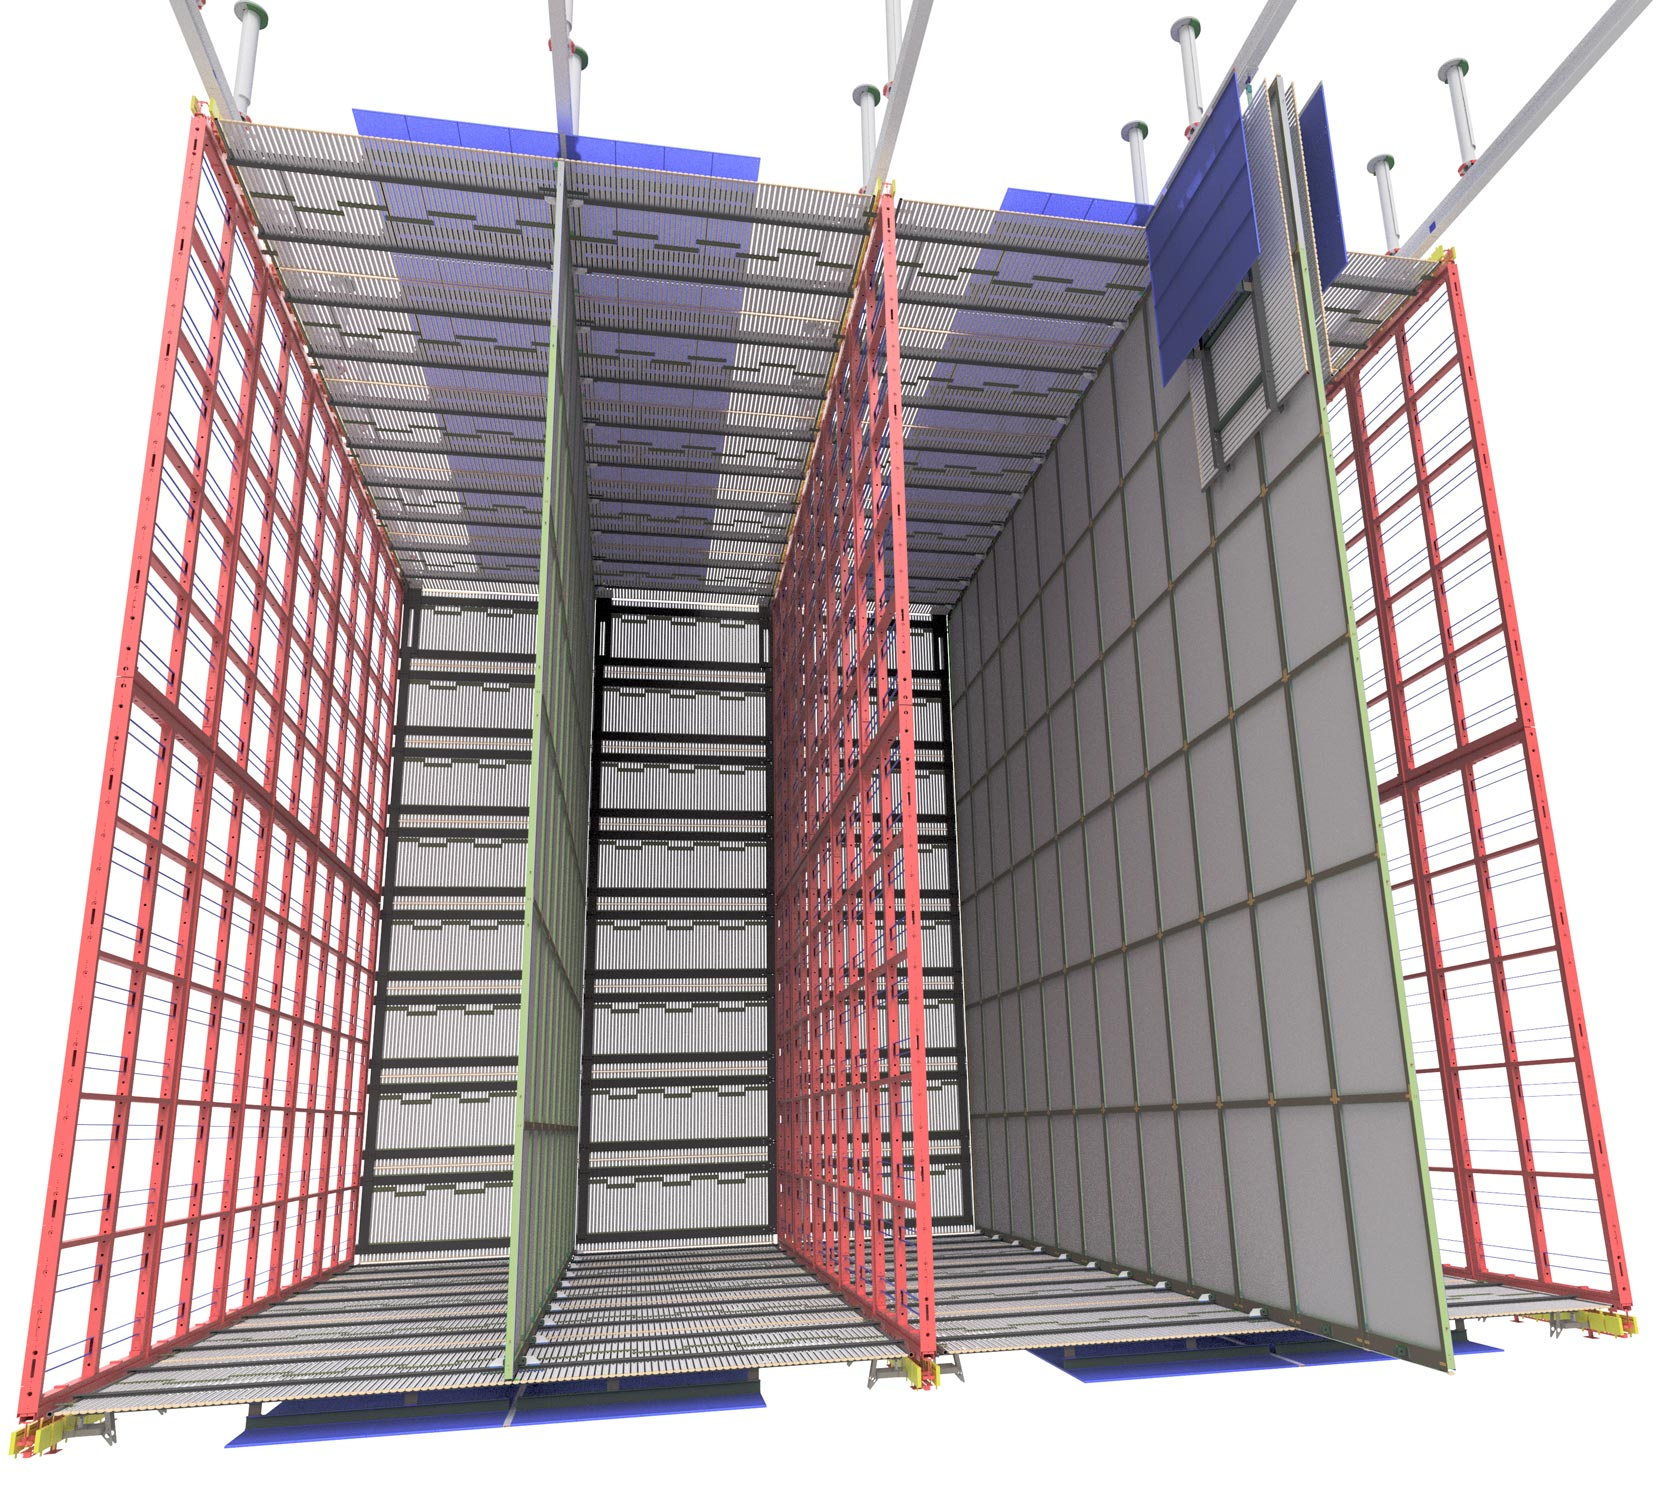
\includegraphics[width=0.95\textwidth]{dune_sp_fd.jpg}
\end{dunefigure}

%%%%%%%%%%%%%%%%%%%%%%%%%%%%
%\subsection{High Voltage System Scope}
%\label{sec:fdsp-hv-scope}

The scope of the \single \dword{hv} system, provided by the DUNE \dword{hvs} consortium, includes the selection and procurement of materials for, and the fabrication, testing, delivery, and installation of systems to generate, distribute, and regulate the voltages that
create a stable and precise \efield{} within a \dword{spmod}. 

The \dword{hv} system consists of components both exterior and interior to the cryostat. The voltage generated at the \dword{hv} power supplies passes through the cables, filters, and the \dword{hv} \fdth into the cryostat. From the point of delivery into the cryostat, components that form part of the \dword{tpc} structure further distribute the voltage. The internal \dword{hv} components in fact form a large fraction of the total internal structures of the \dword{tpc} itself, and  
 %largely 
 effectively bound the  fiducial volume of the %experiment 
 \dword{detmodule}. %The \dword{hv} system plays a key role in determining the event rate for all DUNE physics processes.

The \dword{sp} \dword{hv} system consists of
\begin{itemize}
\item \dword{hv} power supplies, cables, filters, and feedthrough;
\item \dword{cpa} array;
\item \dword{topfc}, \dword{botfc}, and \dwords{gp}; and
\item \dword{ewfc}.
\end{itemize}


The system operates at the full range of voltages, %all voltages, from the highest 
%maximum 
$-$\sptargetdriftvoltpos to ground, inside the \dword{tpc} volume. 

The  \dword{sp} and  \dword{dp} modules will implement similar designs for some
 of the \dword{hv} system components, %including the \dwords{fc} profiles and supporting FRP beams, and the voltage divider boards. More details can be found in   
 in particular, aspects of the \dword{fc} and its supporting beams. This chapter describes the  \dword{sp} versions. 
 
%%%%%%%%%%%%%%%%%%%%%%%%%%%%
\subsection{Design Specifications}
\label{sec:fdsp-hv-des-consid}

The working principle of the \dword{lartpc} relies on the application of a very uniform strong \efield in ultra-pure \dword{lar}.  A number of detector performance parameters benefit from such an \efield in ways that directly support the core components of the DUNE physics program.  Some of these are examined in detail in Volume~\volnumberphysics{}, \voltitlephysics{}.  Here we present a qualitative description of \efield impacts on physics to set context.

Since free electron drift velocity in \dword{lar} is a function of \efield, a uniform \efield leads to a simple time versus position mapping along the drift direction, enabling precise and efficient \threed reconstruction.  This allows, for example, the establishment of a well defined fiducial volume for beam neutrino events reconstructed in the \dword{fd}.  Since a neutrino \dword{cpv} measurement or neutrino \dword{mh} test at root consists of the comparison of normalized spectra for electron and muon neutrino and antineutrinos interactions in the fiducial volume of the \dword{fd} as projected from the \dword{nd}, fiducial volume characterization is critical.   

The optimal \efield range at which to operate the \dword{lartpc} is a trade-off  of detector performances that improve with increasing field against others that degrade. For instance, spectral information is necessary to separate \dword{cp} and \dword{mh} effects, necessitating efficient tracking and shower reconstruction and good energy resolution. To accomplish this, higher E field strength is generally better; more free charge is created at the ionization points, as electron-ion recombination decreases at higher fields, improving \dword{s/n} and calorimetry. 


Drift times are reduced, resulting in less free electron capture from residual electronegative impurities, and hence better \dword{s/n}, even under less than optimal purity conditions.  Spatial resolution improves, as free electron diffusion (proportional to the square root of the drift time) lessens. 

Higher free charge production and lower electron capture allows for lower detection thresholds for components of electromagnetic showers, improving shower energy reconstruction. Lower detection thresholds also lead to higher detection efficiency for MeV-scale electron, photon, and neutron signatures of low-energy $\nu_e$ interactions from \dword{snb} events.  

The electron-ion recombination more strongly affects highly ionizing particles, usually protons.  With decreased recombination, less saturation of free charge production occurs,  leading to better particle identification and more precise energy measurements.  Lower recombination particularly aids in proton-kaon separation by $dE/dx$, a key component of a search for $p\rightarrow K^+ \nu$ baryon decay events. 

However, the \efield should not be raised beyond certain limits. For example, while free charge production increases with \efield, scintillation photon production decreases, resulting in fewer photons available for triggering and determination of $t_0$. Two-track separation can degrade if the drift velocity is increased while keeping the anode wire separation and electronic wave form sampling frequency fixed. The distance between the \dword{tpc} boundaries and the cryostat walls might  need to be increased for very high \efield{}s to prevent electrostatic discharge. This would in turn reduce the fraction of \dword{lar} in the \dword{fv}. The impacts of the first two effects are modest, and all effects are subsidiary to technical challenges in the delivery of high voltage to the cryostat and the maintenance of highly stable  \dword{hv}  surfaces for multiple decades of operation. These challenges require development of non-commercial cryogenic \dword{hv} feedthroughs, \dword{hv} ripple-repression through custom \dword{hv} \dword{r-c} circuits, careful construction and deployment of \dword{hv} cables, redundant \dword{hv} connections, high-precision monitoring, and best practices at all stages of design, installation, and operation.
%end insert

%More quantitative result will be provided by the Physics WG.

To the best of present common knowledge, the response and stability of a \dword{lartpc} to \dword{hv} is strongly dependent on many boundary conditions that are not fully related to the  \dword{hv} design. There are for instance hints and tests that suggest that gas bubble formation as well as residual dust circulating in the \dword{lar} are  primary sources of \dword{hv} instability. Insulator charging up can also affect \dword{hv} performance in the long term.  
Finally, because we found no information on applying \SI{-180}{\kV} in an \dword{lar} detector, our approach to designing the \dword{hv} system relied heavily on past experience, applying in addition sufficient safety margins from previous designs. \dword{pdsp} has provided experience and understanding of \dword{hv} behavior, giving us confidence that the upgraded design documented in this \dword{tdr} is appropriate for underground long-term operation.  

Two decades of design and operational experience that began with \dword{icarus} have established that a \SI{500}{V/cm} field is an appropriate trade-off value that can be realistically achieved through utilization of cost-effective design and construction methods. In practice, achieving this design goal has been challenging as the drift distance has been progressively increased to the 
\SI{3.5}{m} foreseen for the \dword{spmod}, and overall detector optimization has proved to be important. For example, \dword{microboone} operates  at \SI{273}{V/cm} (lower than its nominal value of \SI{500}{V/cm}) and is able to operate well by exploiting its very high argon purity, (characterized by an electron lifetime in excess of 15 ms), as well as an excellent \dword{s/n} ratio from the \dword{fe} \dword{ce}.  
\dword{microboone} (and a number of other noble liquid \dwords{tpc}) compensated for electrostatic instability problems by achieving higher purity, and \dword{dune} might well operate in this mode during its run. 

In \dword{dune}, the minimum requirement of the drift \efield has been set to \mindriftfield, with a goal 
of \mindriftfieldgoal for long-term stable operation. With good free electron lifetime (>\SI{10}{ms}), and the electronics \dword{s/n} demonstrated in \dword{pdsp}, experience shows that \dword{dune} will be able to operate above \SI{250}{V/cm}. The advantage of running at higher \efield is that the lower electron-ion recombination rate and the higher electron drift velocity can compensate for any lower purity conditions that could arise during the planned operation period.

 Running \dword{pdsp} at a higher \dword{hv} value (as allowed by \dword{hv} cables and filtering systems) is under consideration to gain better understanding of the \dword{hv} stability issues.

Positive \dword{protodune} experience (see  Section~\ref{sec:fdsp-hv-protodune-lessons}) indicates that the \SI{500}{V/cm} \efield goal is within reach. This goal, combined with high \dword{lar} purity and a large \dword{s/n} ratio, will allow  a wide range of possible operating points to optimize detector performance for maximum physics potential over decades of stable conditions and very high live-time. 
The specification minimum of \SI{250}{V/cm} will provide adequate detector performance, assuming achievable purity and electronics parameters. 

The \dword{hv} system is designed to meet the physics requirements of the \dword{dune} experiment,  both physical  (e.g., \efield{}s that allow robust event reconstruction) and operational (e.g., avoiding over-complication that could affect 
the time available for collecting neutrino events). 
The important requirements and specifications for the \dword{hv} system are given in Table~\ref{tab:specs:SP-HV}. 

% This file is generated, any edits may be lost.

\begin{longtable}{p{0.14\textwidth}p{0.13\textwidth}p{0.18\textwidth}p{0.22\textwidth}p{0.20\textwidth}}
\caption{Specifications for SP-HV \fixmehl{ref \texttt{tab:spec:SP-HV}}} \\
  \rowcolor{dunesky}
       Label & Description  & Specification \newline (Goal) & Rationale & Validation \\  \colhline

   \newtag{SP-FD-1}{ spec:min-drift-field }  & Minimum drift field  &  $>$\,\SI{250}{ V/cm} \newline ( $>\,\SI{500}{ V/cm}$ ) &  Lessens impacts of $e^-$-Ar recombination, $e^-$ lifetime, $e^-$ diffusion and space charge. &  ProtoDUNE \\ \colhline
    
   
  \newtag{SP-FD-2}{ spec:system-noise }  & System noise  &  $<\,\SI{1000}\,e^-$ &  Provides $>$5:1 S/N on induction planes for  pattern recognition and two-track separation. &  ProtoDUNE and simulation \\ \colhline
    
   
  \newtag{SP-FD-3}{ spec:light-yield }  & Light yield  &  $>\,\SI{20}{PE/MeV}$ (avg), $>\,\SI{0.5}{PE/MeV}$ (min) &  Gives PDS energy resolution comparable that of the TPC for 5-7 MeV SN $\nu$s, and allows tagging of $>\,\SI{99}{\%}$ of nucleon decay backgrounds with light at all points in detector. &  Supernova and nucleon decay events in the FD with full simulation and reconstruction. \\ \colhline
    
    \\ \rowcolor{dunesky} \newtag{SP-FD-4}{ spec:time-resolution-pds } & Name: Time resolution \\
    Description & The time resolution of the photon detection system shall be less than 1 microsecond in order to assign a unique event time.   \\  \colhline
    Specification (Goal) &  $<\,\SI{1}{\micro\second}$  ( $<\,\SI{100}{\nano\second}$ ) \\   \colhline
    Rationale &   Enables \SI{1}{mm} position resolution for \SI{10}{MeV} SNB candidate events for instantaneous rate $<\,\SI{1}{m^{-3}ms^{-1}}$.  \\ \colhline
    Validation &   \\
   \colhline

   \newtag{SP-FD-5}{ spec:lar-purity }  & Liquid argon purity  &  $<$\,\SI{100}{ppt} \newline ($<\,\SI{30}{ppt}$) &  Provides $>$5:1 S/N on induction planes for  pattern recognition and two-track separation. &  Purity monitors and cosmic ray tracks \\ \colhline
    
    \\ \rowcolor{dunesky} \newtag{SP-FD-11}{ spec:hvs-field-uniformity } & Name: Drift field uniformity due to HVS \\
    Description & Design of TPC cathode and FC components shall ensure uniform field.  Production tolerances shall be set so as to maintain flatness of component surfaces and, by extension, the shape of the drift field volume.   \\  \colhline
    Specification &  $<\,\SI{1}{\%}$ throughout volume \\   \colhline
    Rationale &   High reconstruction efficiency.  \\ \colhline
    Validation & ProtoDUNE and simulation  \\
   \colhline

   
  \newtag{SP-FD-12}{ spec:hv-ps-ripple }  & Cathode HV power supply ripple contribution to system noise  &  $<\,\SI{100}e^-$ &  Maximize live time; maintain high S/N. &  Engineering calculation, in situ measurement,   ProtoDUNE \\ \colhline
    
   
  \newtag{SP-FD-16}{ spec:det-dead-time }  & Detector dead time  &  $<\,\SI{0.5}{\%}$ &  Meet physics goals in timely fashion. &  ProtoDUNE \\ \colhline
    
    \\ \rowcolor{dunesky} \newtag{SP-FD-17}{ spec:cathode-resistivity } & Name: Cathode resistivity \\
    Description & The cathode resistivity shall ensure that in the event of an HV discharge, the release of the large stored energy is spread out over time.    \\  \colhline
    Specification (Goal) &  $>\,\SI{1}{\mega\ohm/square}$  ( $>\,\SI{1}{\giga\ohm/square}$ ) \\   \colhline
    Rationale &   Detector damage prevention.  \\ \colhline
    Validation & ProtoDUNE  \\
   \colhline

    \\ \rowcolor{dunesky} \newtag{SP-FD-24}{ spec:local-e-fields } & Name: Local electric fields \\
    Description & The integrated detector design shall minimize potential pathways for HV discharges.   \\  \colhline
    Specification &  $<\,\SI{30}{kV/cm}$ \\   \colhline
    Rationale &   Maximize live time; maintain high S/N.  \\ \colhline
    Validation & ProtoDUNE  \\
   \colhline


   
  \newtag{SP-HV-1}{ spec:power-supply-stability }  & Maximize power supply stability  &  $>\,\SI{90}{\%}$ uptime &  Collect data over long period with high uptime. &  ProtoDUNE \\ \colhline
    
    
   \newtag{SP-HV-2}{ spec:hv-connection-redundancy }  & Provide redundancy in all \dword{hv} connections.  &  Two-fold \newline ( Four-fold ) &  Avoid interrupting data collection. &  Assembly QC \\ \colhline
    


\label{tab:specs:SP-HV}
\end{longtable}  %a hanging "the" was discovered?

We note that specification SP-FD-1 is discussed in the text above Table~\ref{tab:specs:SP-HV}. SP-FD-2  is met in case of stable \dword{hv} operation (lessons from \dword{pdsp}). The noise contribution from \dword{hv} instabilities is unclear and under investigation with \dword{pdsp}. The remaining requirements specific to the \dword{hv} system, summarized here, are all addressed and referred to in the remainder of this chapter. 


\begin{itemize}
\item SP-FD-11: Non-uniformity could be due to defects in resistor chains; muon and laser calibrations will mitigate this effect. [Section~\ref{sec:fdsp-hv-des-fc}] %1.4 Field Cage
\item SP-FD-12: Lessons learned from \dword{pdsp} demonstrate that the present filtering scheme is adequate. [\ref{sec:fdsp-hv-des-hvps}, \ref{sec:fdsp-hv-des-fc-profiles}] %1.2 HV Power Supply and Feedthrough , 1.4.1 Field Cage Profiles 
%\item SP-FD-16: This downtime requirement is already met in \dword{pdsp}; the much lower ionization density in underground operation and optimization in the design (\dword{fc} to \dword{gp} distance) will ensure meeting the requirement even in the case of the much wider detector surface.  
\item SP-FD-17: The \dword{cpa} design is based on few \si{\mega\ohm}/square resistivity surfaces. Such surfaces have been demonstrated in \dword{pdsp} to be adequate to prevent fast discharges that could potentially damage \dword{ce} and the cryostat (no event was ever recorded). Underground operation will allow higher resistivity, thus further slowing down the potential release of stored energy. [\ref{sec:fdsp-hv-cpa-arrays}, \ref{sec:fdsp-hv-des-fc-profiles}] %1.3 CPA Arrays, 1.4.1 Field Cage Profiles
\item SP-FD-24 is met by calculation in \dword{pdsp}. In the present design, the \efield in the critical region between \dword{fc} and \dword{gp} is further reduced. [\ref{sec:fdsp-hv-des-fc-profiles}, \ref{sec:fdsp-hv-design-interconnect}] %1.4.1 Field Cage Profiles , 1.5 Electrical Interconnections 
\item SP-FD-29, 30: These uptime requirements are already met in \dword{pdsp}; the much lower ionization density in underground operation and optimization in the design (\dword{fc} to \dword{gp} distance) will ensure meeting the requirement even in the case of the much wider detector surface. 
\item SP-HV-1: The \dword{hv} distribution and filtering has been tested in \dword{pdsp}; the design of these items will be revised to minimize long-term degradation and maintenance requirements.  [\ref{sec:fdsp-hv-des-fc-profiles}] %1.4.1 Field Cage Profiles
\item SP-HV-2: Two-fold redundant connections to the \dword{cpa} are foreseen. The \dword{hv} feedthrough and its connection to the \dword{cpa} is designed in such a way that it could be extracted and replaced even with the detector filled with \dword{lar} (based on \dword{icarus} experience). [\ref{sec:fdsp-hv-cpa-arrays}, \ref{sec:fdsp-hv-design-interconnect}] %1.3 CPA Arrays, 1.5 Electrical Interconnections 
\end{itemize}
%%%%%%%%%%%%%%%%%%%%%%%%%%%%
\subsection{Design Overview}
\label{sec:fdsp-hv-des}

%%%%%%%%%%%%%%
\subsubsection{Cathode Plane Assembly (CPA) Arrays}
\label{sec:fdsp-hv-des-cpa}

\dword{cpa} arrays are made up of adjacent resistive cathode panels, secured in frames and connected by an \dword{hv} bus. \dword{hv} cups are mounted at both ends to receive input from the power supply.

Two \dword{cpa} arrays span the length and height of the \dword{spmod}, as shown in Figure~\ref{fig:dune_sp_fd}. %Given the modular design, 
Each array is assembled from a set of \num{25} adjacent full-height \dword{cpa} planes, %which in turn are constructed of smaller pieces.  Each plane is a set 
each of which consists of two adjacent full-height panels. % (full height, half length, as measured along the \dword{detmodule} length). 
Each panel consists of three stacked units, approximately \SI{4}{\m} in $y$ (height) by \SI{1.2}{\meter} in the $z$-coordinate (parallel to beam). %long.
A unit consists of two %half-height 
vertically stacked \dwords{rp} framed by  \frfour\footnote{NEMA grade designation for flame-retardant glass-reinforced epoxy laminate material, multiple vendors, National Electrical Manufacturers Association\texttrademark{},  \url{https://www.nema.org/pages/default.aspx}.} members. 
The \dword{hv} cathode components are listed in Table~\ref{tab:cpaparts} and will hereafter be referred to by their names as defined in this table.

\begin{dunetable}
[HV cathode components]
{p{0.4\textwidth}p{0.12\textwidth}
p{0.12\textwidth}p{0.32\textwidth}}
{tab:cpaparts}
{\dword{hv} cathode components} %plane 
Component and Quantity &  Length (z) & Height (y) & Per \dword{spmod} \\ \toprowrule
\dword{cpa} array (2 per \dword{spmod}) & \SI{58}{\meter} & \SI{12}{\meter} & 2  \\ \colhline
\dword{cpa} plane (25 per \dword{cpa} array)  & \SI{2.3}{\meter}  &\SI{12}{\meter} & 50  \\ \colhline
\dword{cpa} panel (2 per \dword{cpa} plane)  & \SI{1.2}{\meter}   & \SI{12}{\meter} & 100  \\ \colhline
\dword{cpa} unit (3 per \dword{cpa} panel)  & \SI{1.2}{\meter}  & \SI{4}{\meter} & 300 \\ \colhline
\dword{rp} (2 per \dword{cpa} unit)  & \SI{1.2}{\meter}  & \SI{2}{\meter} & 600 \\
\end{dunetable}
The \dwords{rp} are made of a highly resistive material. % and assembled into frames.
An  installation rail supports the \dword{cpa} panels from above through a single mechanical link. % changed panels to CPA Panels - SRM

The cathode bias is provided by an external \dword{hv} power supply through an \dword{hv} \fdth connecting to the \dword{cpa} array %plane 
inside the cryostat. 
 
%%%%%%%%%%%%%%
\subsubsection{Field Cage}
\label{subsec:fdsp-hv-des-fc}

%Anne augmented intro sentence from pdune tdr
In the \dword{spmod}, an \dword{fc} covers the top, bottom, and endwalls of all the drift volumes, thus providing the necessary
boundary conditions to ensure a uniform \efield, unaffected by the presence of the cryostat walls. % on both sides of each \dword{cpa} plane. 
The \dword{fc} is made of adjacent extruded aluminum open profiles (electrodes) running perpendicular to the drift field and set at increasing potentials along the \spmaxdrift drift distance from the \dword{cpa} \dword{hv} (\SI{-180}{kV}) to ground potential at the \dword{apa} sensor arrays. %planes. 

The \dword{fc} modules come in two distinct types: the identical top and bottom modules, which are assembled to run the full length of the \dword{detmodule}, and the \dword{ewfc} modules, 
which are assembled to complete the detector at either end. %Both types of modules are constructed of extruded aluminum open 
The profiles in both types of modules are supported by \dword{frp}\footnote{Fiber-reinforced plastic, a composite material made of a polymer matrix reinforced with fibers, many vendors.} (fiber-reinforced plastic) structural beams.  

The \dword{topfc} and \dword{botfc} modules extend nominally  \SI{2.3}{\meter} in $z$ and \SI{3.5}{\meter} in $x$; the top and bottom of the \dword{spmod} each requires 25 modules lengthwise in $z$ and four across in $x$.  The \dword{ewfc} modules are \SI{3.5}{\meter} wide by \SI{1.5}{\meter} in high; each endwall requires four adjacent stacks, eight units high. A \dword{gp} consisting of modular %tiled, 
perforated stainless steel sheets % panels %is mounted on 
runs along the outside surface of each of the %top and bottom \dword{fc} modules 
\dword{topfc} and \dword{botfc}, with a \SI{30}{\centi\meter} clearance. The \dword{ewfc} modules do not require a \dword{gp} because the distance to the cryostat wall is sufficient, approximately \SI{2}{\meter}.

To provide a linear voltage gradient within each drift volume, %between each set of facing %cathode and anode planes \dword{cpa} and \dword{apa} arrays, 
a chain of resistive divider boards connects the adjacent pairs of aluminum profiles along each \dword{fc} module. 

Table~\ref{tab:fcparts} lists the \dword{fc} components.
\begin{dunetable}
[HV field cage components]
{p{0.37\textwidth}p{0.13\textwidth}p{0.07\textwidth}p{0.07\textwidth}p{0.07\textwidth}
p{0.1\textwidth}p{0.08\textwidth}}
{tab:fcparts}{\dword{hv} field cage components}
Component & Count & Length (z) & Width (x) & Height (y) & Submodules & Grand Total \\ \toprowrule
%\dword{fc} (Top/Bottom Field Cage) & 200 & 2.3 m & 3.5 m & - & 57 & 200 \\ \colhline
\Dword{topfc} modules & 100 (4$\times$25) & 2.3 m & 3.5 m & - & - & 100 \\ \colhline
\Dword{botfc} modules & 100 (4$\times$25) & 2.3 m & 3.5 m & - & - & 100 \\ \colhline
%\dword{fc}-Profiles (per \dword{fc}) & 57 & 2.3 m & - & - & - & 11400 \\ \colhline
Profiles per module \\(all top and bottom module types) & 57 & 2.3 m & - & - & - & 11400 \\ \colhline
\Dword{gp} modules per top or bottom \\ \dword{fc} module & 5 & 2.3 m & 0.7 m & - & - & 1000 \\ \colhline
%EW-Plane (Endwall Field Cage) & 2 & - & 14.4 m & 12 m & 4 & 2 \\ \colhline
\Dword{ewfc} plane & 2 & - & 14.4 m & 12 m & 4 & 2 \\ \colhline
%EW (per EW-Plane) & 4 & - & 3.5 m & 12 m & 8 & 8 \\ \colhline
%\Dwords{ewfc} per \dword{ewfc} plane  & 4 & - & 3.5 m & 12 m & 8 & 8 \\ \colhline
\Dword{ewfc} modules per \dword{ewfc} & 32 & - & 3.5 m & 1.5 m & - & 64 \\ \colhline
Profiles per \dword{ewfc} module & 57 & - & - & 1.5 m & - & 3648 \\

\end{dunetable}



%%%%%%%%%%%%%%
\subsubsection{Electrical Considerations}
\label{sec:fdsp-hv-des-elec}

As shown in Figure~\ref{fig:dune_sp_fd}, the outer \dword{apa} arrays face the cryostat walls, and the \dword{cpa} arrays are installed between the \dword{apa} arrays in two of the three interior positions (A-C-A-C-A).
In this configuration, as opposed to C-A-C-A-C,  most of the cathode plane surfaces are far away from the grounded cryostat walls, reducing electrostatic breakdown risks and decreasing the total energy stored in the \efield to \SI{800}{J}.

\begin{dunefigure}[Electric field distribution in the TPC]
{fig:e-field-distribution}
{A simplified cross sectional view of an outer drift volume of the \dword{tpc} showing the distribution of the static \efield (in V/m).  Since the electrostatic potential energy is proportional to $E^2$, most of the energy is stored between the \dword{fc} modules and their facing \dwords{gp}.   }
\centering
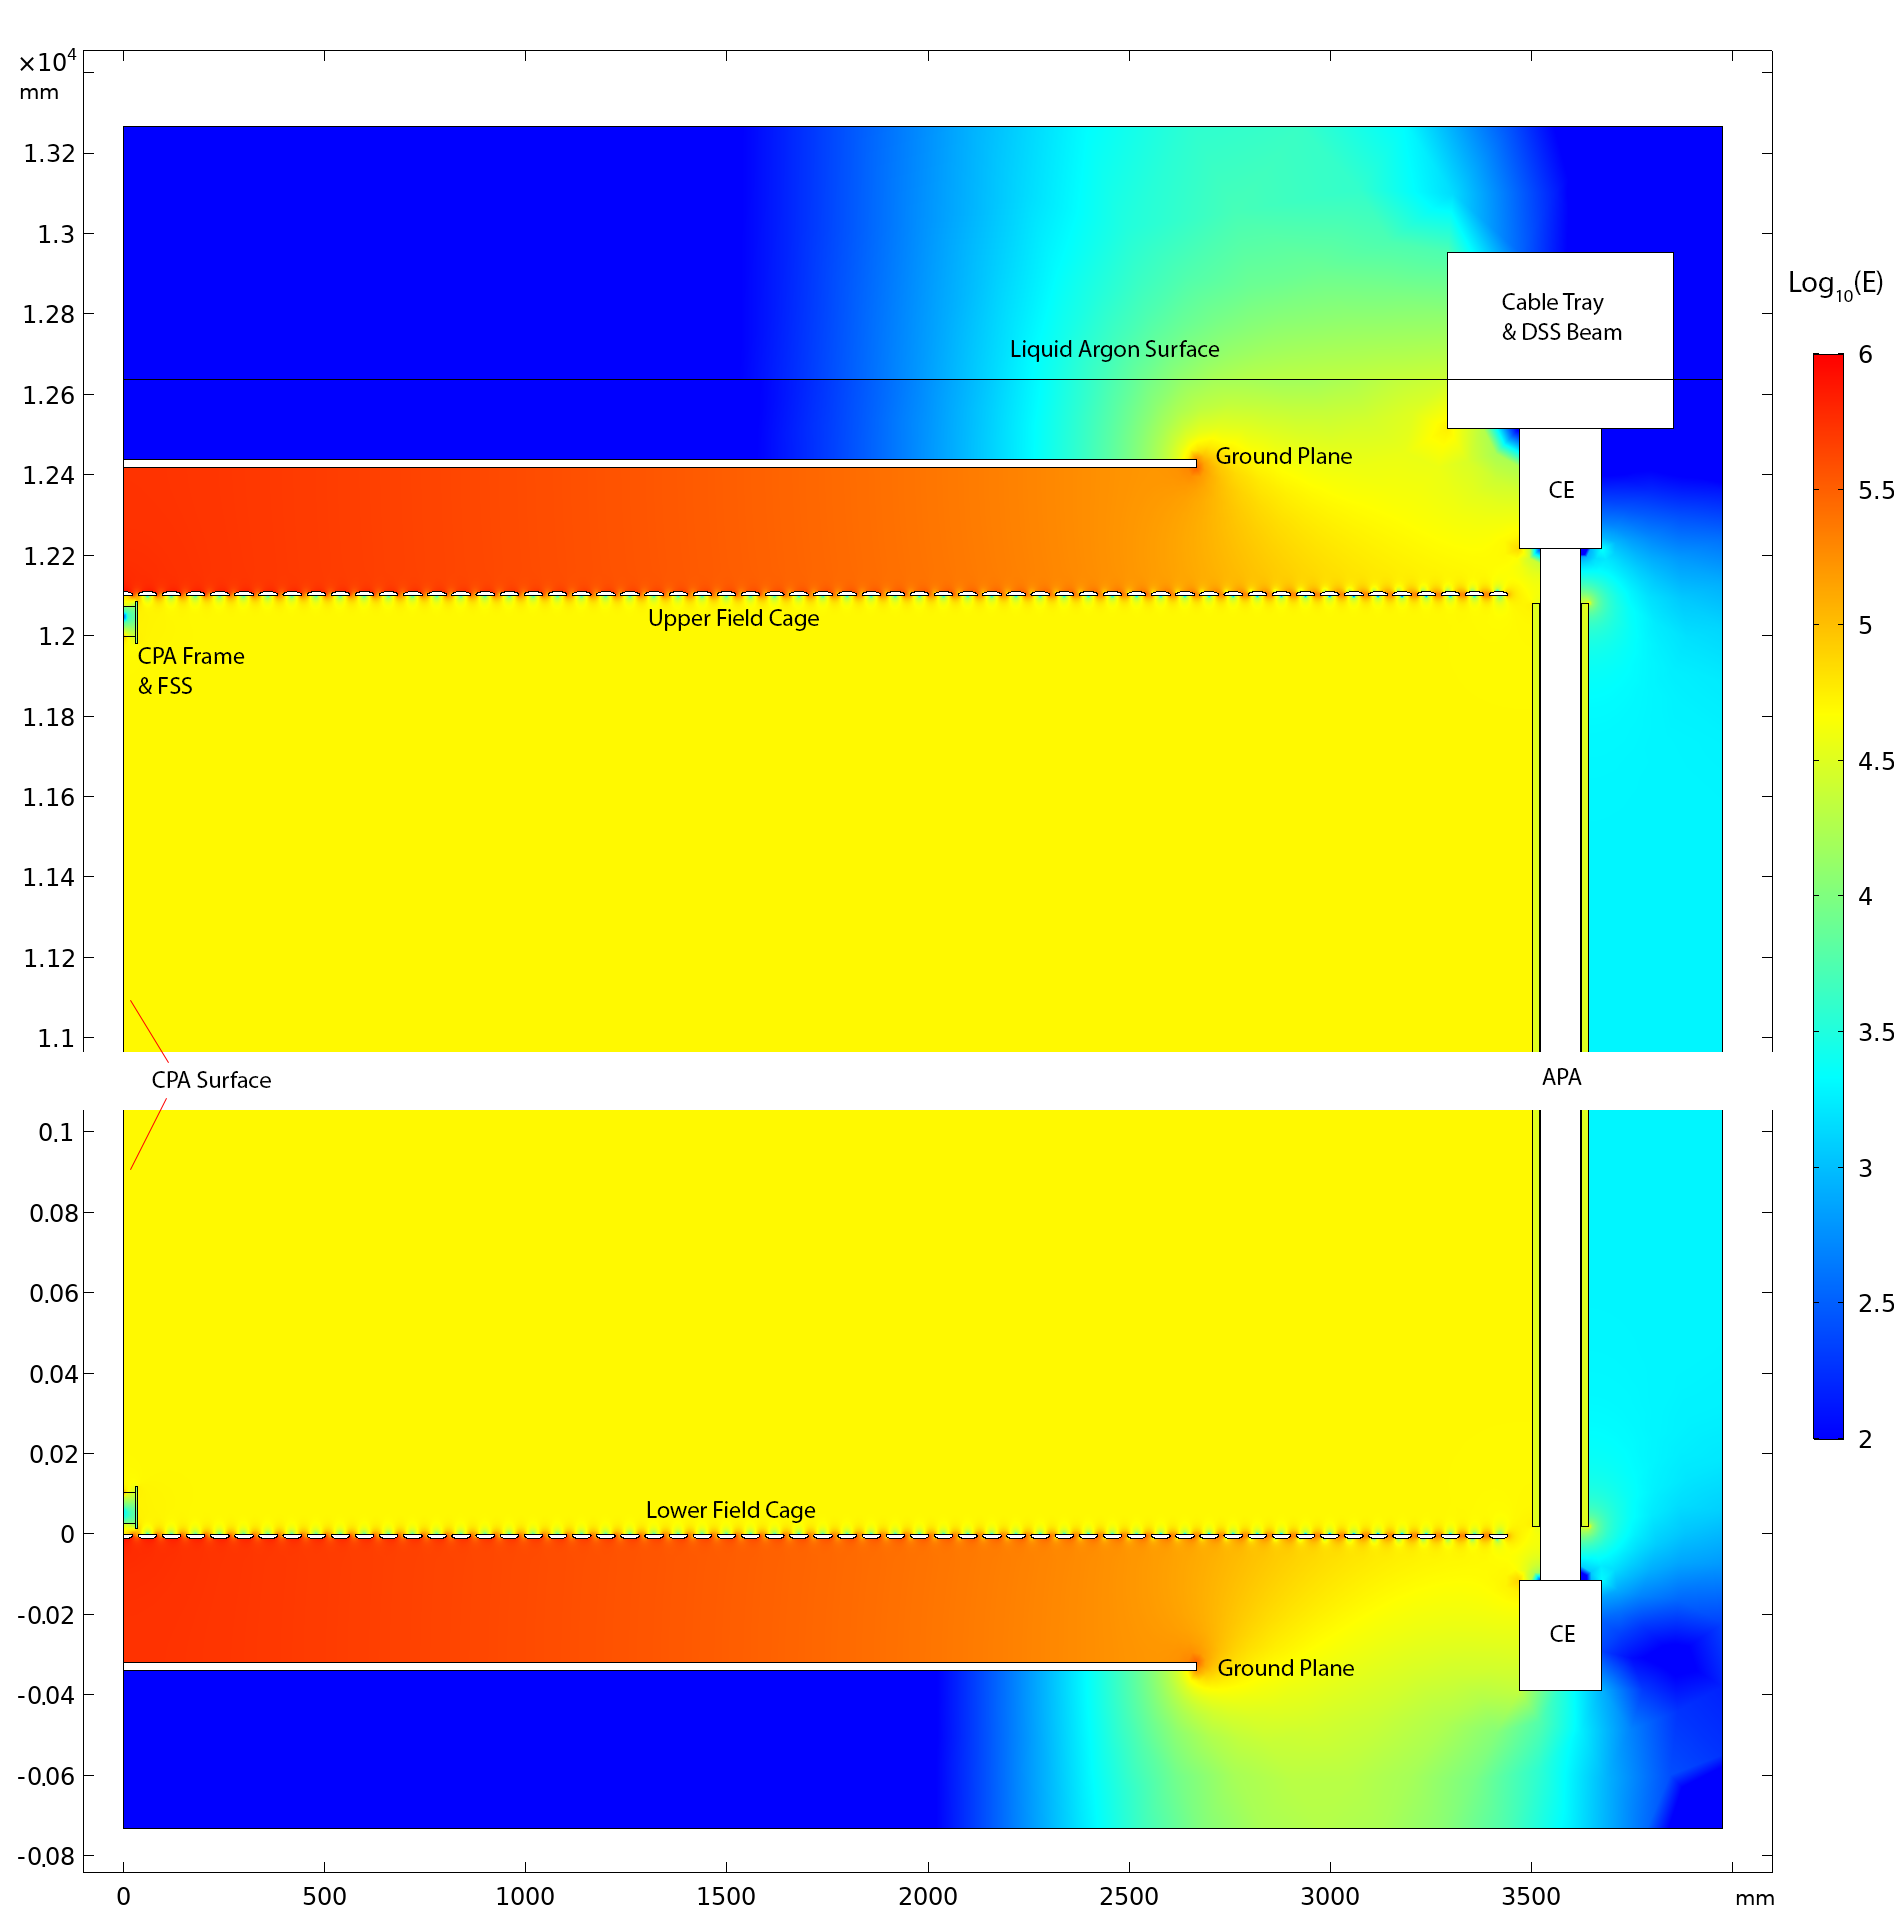
\includegraphics[width=0.7\textwidth]{graphics/E_Field_Distribution.png} 
\end{dunefigure}

Figure~\ref{fig:e-field-distribution} maps out the \efield strength over a cross section of a drift volume.  
The energy is stored mostly in the high \efield{} region between the \dword{fc} and the facing \dwords{gp}.  In the case of an unexpected \dword{hv} breakdown, the entire \SI{400}{J} associated with one \dword{cpa} array could be discharged to ground,
potentially causing physical damage.
Given the difficulty of predicting the distribution of energy along a discharge path, we treat the possibility of discharged energy, conservatively, as a risk to the TPC components and the cryostat membrane. 

Previous large \dwords{lartpc} (e.g., \dword{icarus} and \dword{microboone}) have used continuous stainless steel tubes as their \dword{fc} electrodes;
however, a continuous electrode in a DUNE \dword{detmodule} would need to be at least \SI{140}{\m} long. This would increase the stored energy in each electrode and, in turn, increase the risk of damage in the case of a discharge. 

Subdividing the \dword{fc} into electrically isolated modules limits the stored energy in each \dword{fc} module, thereby minimizing the risk of damage. Each \dword{fc} module must have its own voltage divider network to create a linear voltage gradient. Dividing the \dword{fc} into mechanically and electrically independent modules also eases the construction and assembly of the \dword{fc} and greatly restricts the extent of drift field distortion caused by a resistor failure on the divider chain of a \dword{fc} module.

An \dword{hv} discharge onto a metallic cathode could cause the electrical potential of the entire cathode surface to swing from its nominal bias (e.g., $-$\sptargetdriftvoltpos) to \SI{0}{V} in a few nanoseconds, inducing a large current into the analog \dword{fe} amplifiers connected to the sensing wires on the \dword{apa}s (mostly to the first induction wire plane channels). 
An internal study\cite{bib:docdb1320} has shown that with a metallic cathode structure, an \dword{hv} discharge could swing the outer wire plane by nearly \SI{100}{V} and inject \SI{0.9}{A} current into the input of the \dword{fe} amplifiers connected to the first induction plane, possibly overwhelming the internal electrostatic discharge (\dword{esd}) protection in the \dword{fe} \dwords{asic}.  

On the other hand, a highly resistive cathode structure can significantly delay the change in its potential distribution in a discharge event due to its large distributed \dword{r-c} time constant. Such a delay reduces both the current flowing through the discharge path and the current induced on the anode readout amplifiers.  The upper limit in the cathode surface resistivity is 
determined by the voltage drop between the center and the edges of the cathode array driven by the ionization current flowing to the cathode.  For example, a surface resistivity of \SI{1}{\giga\ohm}/square  will have a voltage drop less than \SI{1}{V} from the $^{39}$Ar ionization flux at the underground site. Figure~\ref{fig:cpa-frame-discharge} illustrates the two main 
benefits in such a design in an event of \dword{hv} discharge at the edge of the cathode: (1) reducing the rate of transfer of the stored energy in the cathode plane to reduce the risk of damage to the \dword{hvs} and cryostat membrane; and (2) slowing down the change in cathode voltage distribution that capacitively injects charge into the readout electronics.
With a surface resistivity of \SI{1}{\giga\ohm}/square on the entire cathode, the time constant of a discharge is on the order of a few seconds. An \dword{hv} discharge on the edge of the cathode would inject a maximum current of only about 50\,$\mu$A into the \dword{fe} \dwords{asic}, avoiding damage.



\begin{dunefigure}[Simulated CPA discharge event]
{fig:cpa-frame-discharge}
{Simulated discharge event on a highly resistive cathode surface with a surface resistivity of \SI{1}{\giga\ohm}/square. Top:  stored energy on the cathode as a function of elapsed time from an \dword{hv} discharge. 0.2 second after the discharge, only about 15\% of the stored energy contributes to the discharge. Bottom: voltage distribution on a section of the cathode (2.3\,m\,$\times$\,12\,m) 0.2\,s after the discharge at the upper right edge.  Due to the long time constant of the cathode, most of the surface area remains at the \SI{-180}{\kV} operating potential. Only the region close to the discharge site shifts positively toward 0V. Charge injection to the wire readout electronics, proportional to $dV/dt$ averaged over the cathode area facing an \dword{apa}, is therefore greatly suppressed. }
\centering
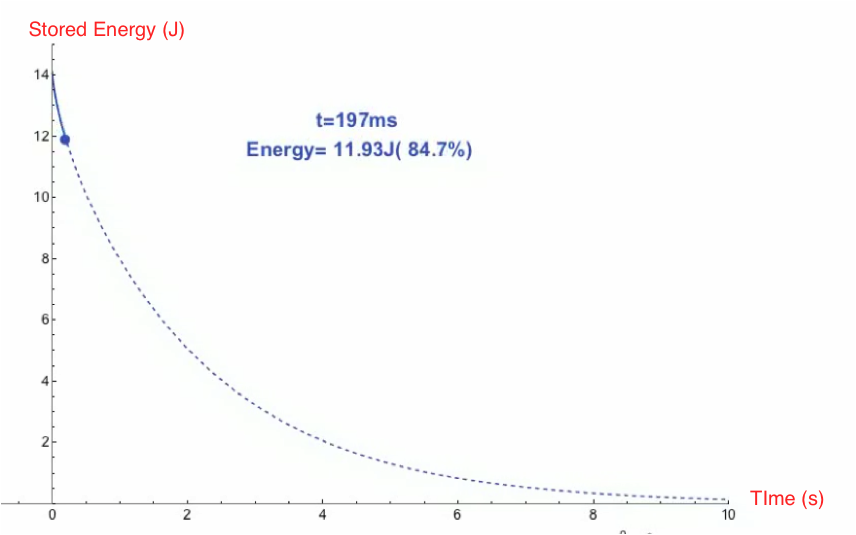
\includegraphics[width=0.7\textwidth,trim=2mm 2mm 2mm 2mm,clip]{A2r} \\ \vspace{20pt}    %update image with red labels, trim border
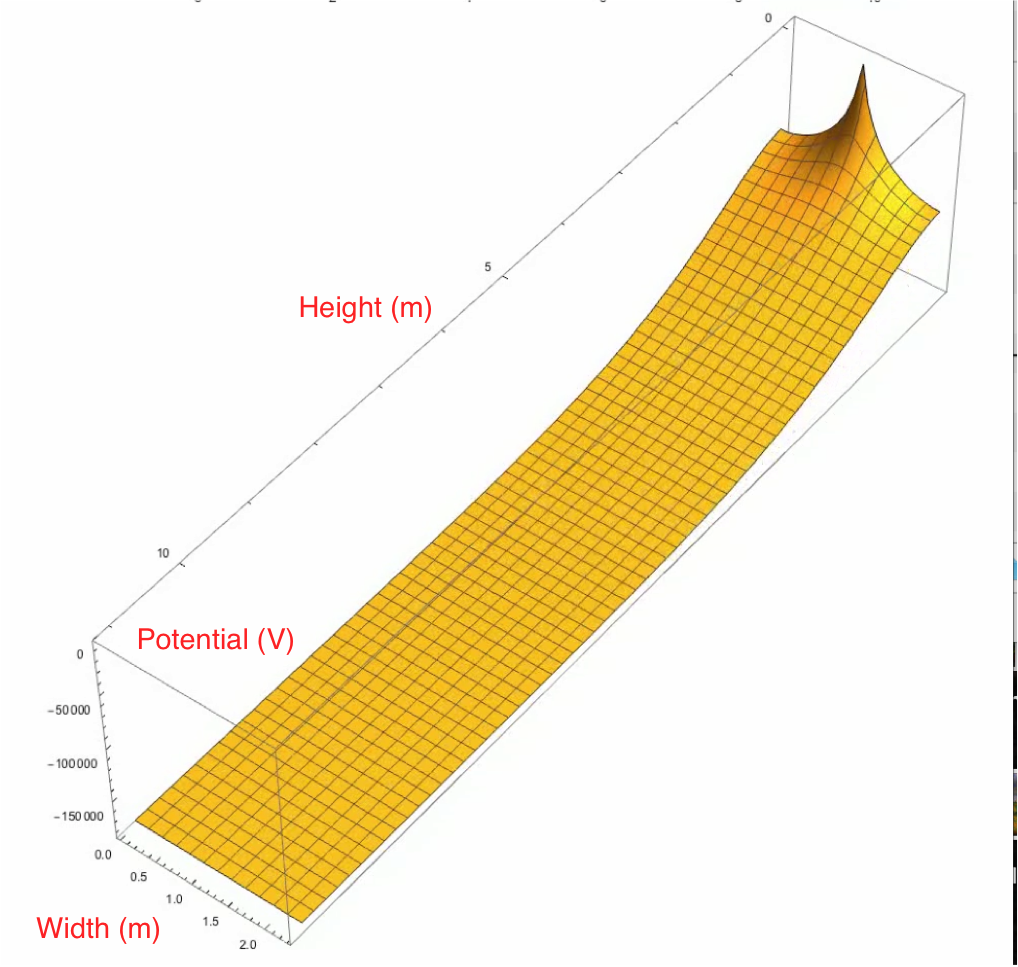
\includegraphics[width=0.6\textwidth,trim=2mm 2mm 2mm 2mm,clip]{A3r}
\end{dunefigure}


%%%%%%%%%%%%%%
\subsubsection{Structural Considerations}
\label{sec:fdsp-hv-des-des-sc}

The frames around the \dword{cpa} panels and the frames supporting the \dword{fc} aluminum profiles  
are made from materials with similar thermal expansion coefficients, minimizing issues of differential thermal expansion. The \dword{fc} frames 
are restrained at only one location.  The \dword{cpa}s and \dword{apa}s support the \dword{topfc} and \dword{botfc} modules, whereas installation rails above the \dword{cpa}s and \dword{apa}s support the \dword{ewfc} modules. 

All structural members of the \dword{cpa}s and \dwords{fc} are made of either \frfour or \dword{frp} with very similar coefficients of thermal expansion (\dword{cte}). However, the structures supporting the \dword{cpa}s and \dwords{fc} are made of stainless steel, with a \dword{cte} about 50\% greater.  To accommodate the mismatch in the \dwords{cte}, small expansion gaps are added between \dword{cpa}s at installation time. These gaps are set during installation between \dword{cpa} panels by adjusting the distance between the \dword{cpa} hanger bars and between \dword{cpa} planes at the top of the \dword{tpc} on the \dword{cpa} beam; these \SI{3}{mm} gaps, 49 of them in total, will disappear once the \dword{tpc} is submerged in \dword{lar}. % at operating temperature.
 
%%%%%%%%%%%%%%
\subsubsection{Design Validation}
\label{sec:fdsp-hv-des-des-val}

Successful \dword{protodune} running and extensive testing has %been performed of 
validated the mechanical and electrical properties of materials selected for the \dword{hv} system.  These are fully documented in references~\cite{bib:docdb2338, bib:docdb1504, bib:docdb1601}. More details follow in Section~\ref{sec:fdsp-hv-protodune}.


Issues identified in earlier testing form the basis of an ongoing R\&D program. 

Operations experience from \dword{pdsp} is summarized in Section \ref{sec:fdsp-hv-protodune}. It revealed some instabilities in the \dword{hvs} operations.  Design changes (see Section \ref{sec:fdsp-hv-des-fc-gp}) have been introduced to the top and bottom \dword{fc} assemblies to further decrease the overall \efield between the profiles and the \dwords{gp}.


%%%%%%%%%%%%%%%%%%
\subsection{HV System Safety}
\label{fdsp-hv-design-safety}

Safety is central to the design of the \dword{hv} system and is the highest priority concern in all phases: fabrication, installation, and operations. Documentation of assembly, testing, transport, and installation procedures is in progress and systematically catalogued. % in the \dword{docdb}. 
Particular attention was paid to these procedures in the design and construction of \dword{pdsp}, with the explicit understanding that they be applicable to the \dword{spmod}. The most critical procedures are also noted in the current \dword{hv} risk assessment. 


The structural and electrical designs for the \dword{spmod} \dword{hv} are closely modeled on designs that were vetted and validated in the \dword{pdsp} construction. 
Prior to \dword{pdsp}, a full-voltage and full-scale \dword{hv} feedthrough, power supply, filtering, and monitoring system were tested at \dword{fnal}, along with the \dword{hv} connection cup and arm,  %(Described in Section?)
after completing full safety reviews. 
These devices worked as designed and were used in \dword{pdsp}. They will be reproduced for the \dword{spmod},  except for specific optimizations described in this chapter. %previous sections.

At full operating voltage, the \dword{fc} stores a substantial amount of energy.
As discussed in Section~\ref{sec:fdsp-hv-des-elec}, the \dword{cpa} is designed to limit the power dissipated during a power supply trip or other failure that unexpectedly drops the \dword{hv}.
Its design has succeeded in tests at full voltage over \num{2}\,m$^2$ surfaces and at larger scale in \dword{pdsp}.  

Integral to the \dword{pdsp} and \dword{spmod} design is the concept of pre-assembled modular panels of field-shaping conductors with individual voltage divider boards. The structural design and installation procedures used in \dword{pdsp} were selected to be compatible with use at the \dword{fd} site and were vetted by project engineers, engineering design review teams, and safety engineers at the \dword{cern}. Any revisions to these designs based on lessons learned in \dword{pdsp}  installation and operations will be reviewed both within the project and by \dword{fnal} \dword{esh} personnel. The safety features of the overall design are on solid footing. 

%%%%%%%%%%%%%%%%%%%%%%%%%%%%
\section {HV Power Supply and Feedthrough}
\label{sec:fdsp-hv-des-hvps}

The \dword{hv} delivery system consists of
\begin{itemize}
\item two power supplies,
\item \dword{hv} cables,
\item filter resistors, and
\item \dword{hv} feedthrough into the cryostat.
\end{itemize}

For \dword{hv} delivery, two power supplies generate the voltage, one for each \dword{cpa} array. 
This separated setup accommodates any necessary different running voltages between the two \dword{cpa} arrays.
The cryostat design has two feedthrough ports for each \dword{cpa} array, one at each end of the cryostat. Correspondingly, two \dword{hv} receiving cups are mounted on the \dword{cpa} array frame. The spare downstream port provides redundancy against any failure of the primary \dword{hv} delivery system. In addition, the \dword{hv} feedthrough is designed to be extracted and replaced in case of misbehavior.

Each \dword{cpa} array separates and services two adjacent drift volumes, 
presenting a net resistance of \SI{1.14}{\giga\ohm} to each power supply. At the nominal \SI{180}{kV} cathode voltage, each power supply must provide \SI{0.16}{mA}. 
The power supply model planned for the \dword{spmod} is similar to that used on \dword{pdsp}.\footnote{Heinzinger, PNC HP300000 \dword{hv} power supply, Heinzinger\texttrademark{} Power Supplies, \url{http://www.heinzinger.com/}.}  
The \dword{hv} cables are commercially available models compatible with the selected power supplies. 

Filter resistors are placed between the power supply and the feedthrough.  Along with the cables, these resistors reduce the discharge impact by partitioning the stored energy in the system.  The resistors and cables together also serve as a low-pass filter reducing 
the \SI{30}{kHz} voltage ripple on the output of the power supply.  With filtering, such supplies have been used successfully in other \dword{lartpc} experiments, such as \dword{microboone} and \dword{icarus}. Figure~\ref{fig:ps_filter_ft_schematic} shows the \dword{hv} supply circuit.

\begin{dunefigure}[Power supply photos and schematic of HV delivery system to the cryostat]  
{fig:ps_filter_ft_schematic}
{Left: Photo of \SI{300}{kV} and \SI{200}{kV} power supplies. %An example (Credit: CERN). 
Right:  A schematic showing the \dword{hv} delivery system to the cryostat. %(Credit:  SEL).  
One of the two filter resistors sits near the power supply; the other sits near the feedthrough.}
\begin{minipage}{\textwidth}%{6in}
  \centering
 $\vcenter{\hbox{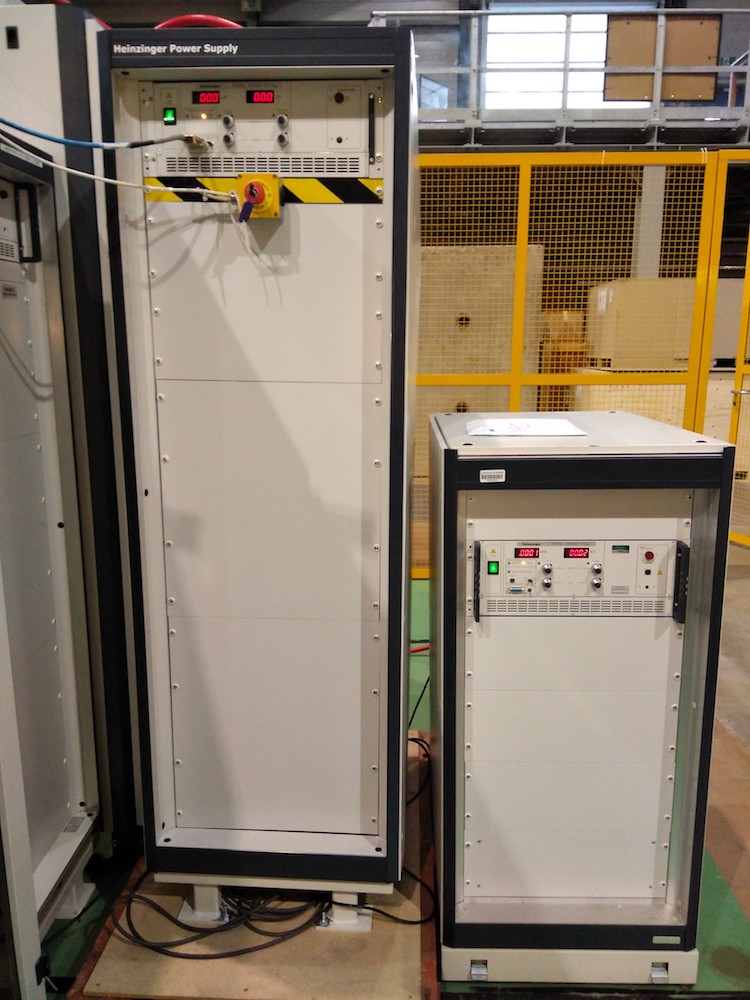
\includegraphics[width=0.25\textwidth]{Power_Supplies_300_and_200.jpg}}}$
 \hspace*{0.001\textwidth}  $\vcenter{\hbox{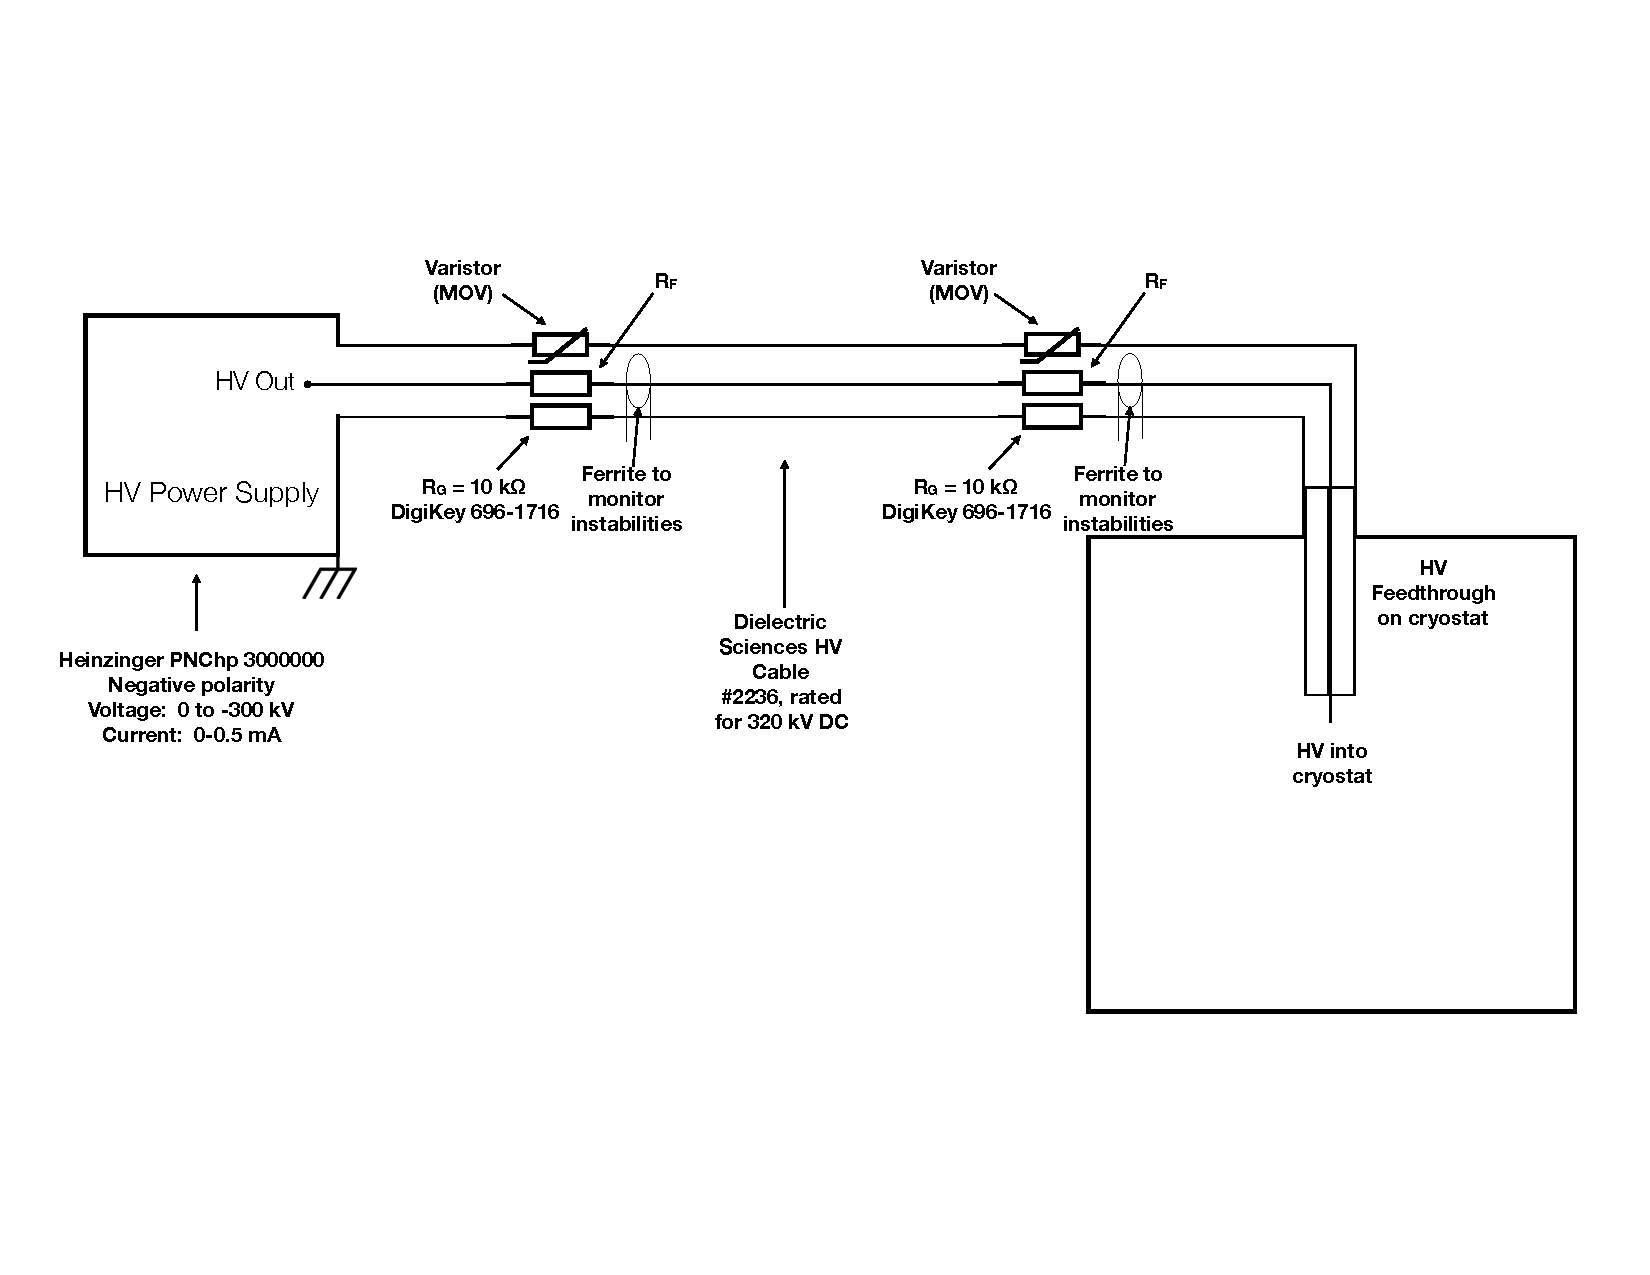
\includegraphics[width=0.7\textwidth]{ps_filter_ft_schematic}}}$
\end{minipage}
\end{dunefigure}
The requirement  
on low electronics noise sets the upper limit of residual voltage ripple on the cathode to be \SI{0.9}{mV}. 

Typically, commercial supplies specify a ripple variation limit of 
\SI{.001}{\%} around an absolute precision in nominal voltage of $\pm\,$\SI{50}{mV}.
%
Assuming cable lengths of \SI{30}{m} and \SI{3}{m} between the filters themselves and between the filter and \fdth, respectively, calculations and experience confirm that resistances as low as a few \si{\mega\ohm} yield the required noise reduction. 

The %current plan for the 
filter resistors are of a cylindrical design. 
Each end of a \dword{hv} resistor is electrically connected to a cable receptacle. 
The resistor %should shall be selected to 
must withstand a large over-power condition.  A cylindrical insulator is placed around the resistor.

The \dword{hv} feedthrough %will be 
is based on the successful ICARUS design \cite{Icarus-T600}, 
which was adapted for \dword{pdsp}.  The voltage is transmitted by a stainless steel center conductor.  On the warm side of the cryostat, this conductor mates with a cable end.  Inside the cryostat, the end of the center conductor has a spring-loaded tip that %will 
contacts a receptacle cup mounted on the cathode, delivering \dword{hv} to the \dword{fc}.  The center conductor of the \fdth is surrounded by ultra-high molecular weight polyethylene (\dword{uhmwpe}), an insulator. This is illustrated in Figure~\ref{fig:filterAndFeedthrough}.

\begin{dunefigure}[Photo and drawing of a HV  feedthrough]{fig:filterAndFeedthrough}
{Photograph and drawing of a \dword{hv} \fdth{}. Photograph shows \dword{pdsp} installation. The distance from the cup to the top surface is approximately \SI{1.3}{\meter}. } 
\begin{minipage}{\textwidth}%{6in}
  \centering
 $\vcenter{\hbox{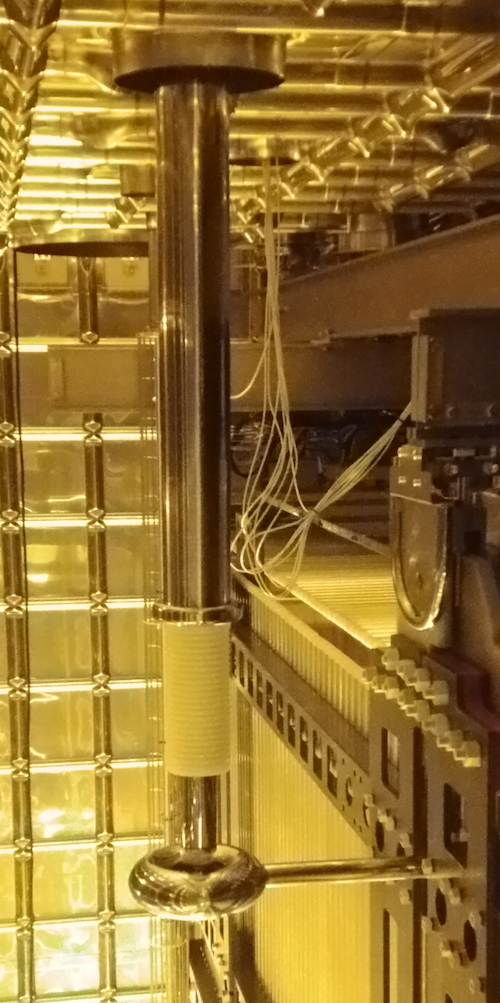
\includegraphics[width=0.16\textwidth]{hv_feedthrough.png}}}$
 \hspace*{0.001\textwidth}  $\vcenter{\hbox{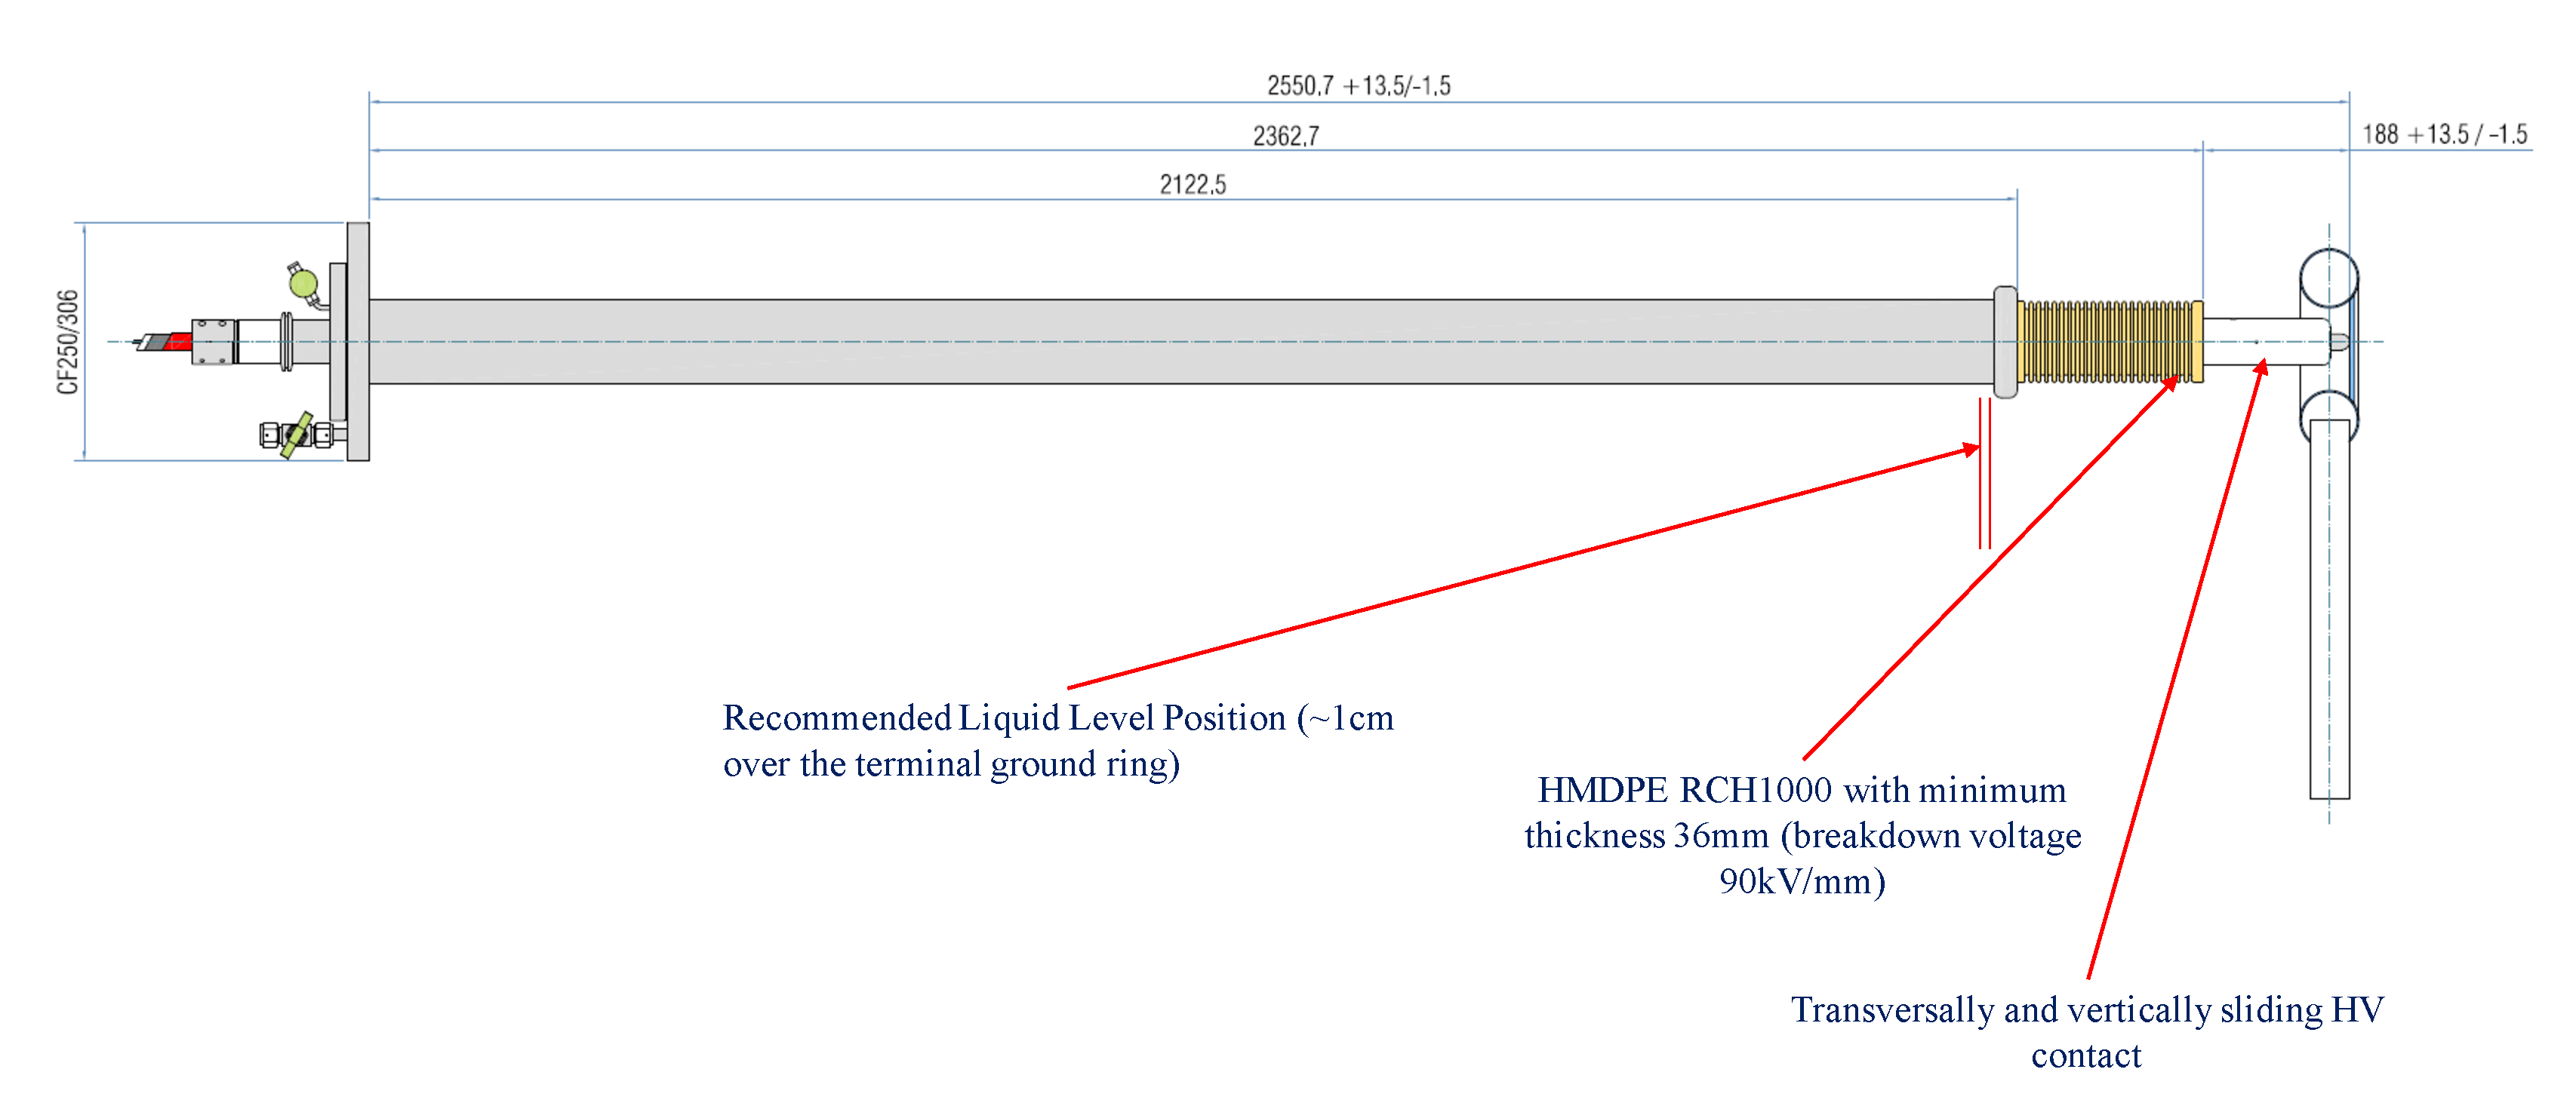
\includegraphics[width=0.82\textwidth]{francosHVFT}}}$
\end{minipage}
\end{dunefigure}

On a feedthrough, to a first approximation, the operating voltage upper bound is set by the maximum \efield{}. This \efield{} can be reduced by increasing the insulator radius.  For the target voltage, the feedthrough uses a \dword{uhmwpe} cylinder of approximately \SI{15}{cm} diameter.  In the gas space and into at least \SI{15}{\centi\meter} of the liquid, the insulator is surrounded by a tight-fitting stainless steel ground tube.  A %\SI{25}{\centi\meter}  
Conflat industry-standard flange is welded onto the ground tube for attachment to the cryostat.

Outside the cryostat, the \dword{hv} power supply and cable-mounted toroids monitor the \dword{hv}.    The power supplies 
have capabilities down to tens of \si{\nano\ampere} in current read-back 
and are able to sample the current and voltage every \SI{300}{\ms}.  The cable-mounted toroids are sensitive to fast changes in current;  
the polarity of a toroid's signal  
indicates the location of the current-drawing feature as either upstream or downstream of it.  Experience from the DUNE \dword{35t} installation suggests that sensitivities to changing currents %with 
are on a timescale between \SIrange{0.1}{10}{\micro\s}.

Inside the cryostat, pick-off points near the anode monitor the current  
in each resistor chain.  Additionally, the voltage of the \dwords{gp} above and below each drift region can diagnose problems via a high-value resistor connecting the \dword{gp} to the cryostat.  In the DUNE \dword{35t}, such instrumentation provided useful information on \dword{hv} stability and locations of %where 
any stray charge flows. %was flowing.


Both commercial and custom \dword{hv} components must be rated for sufficient voltage and must satisfy tests to meet the specifications %requirements 
summarized in Section~\ref{sec:fdsp-hv-des-consid}.  Section~\ref{sec:fdsp-hv-transport-QC} provides further details on these tests.

The resistances in the filters, in combination with the capacitances between the \dword{hv} system and the cathode,
 determine the attenuation of the tens-of-\si{\kilo\hertz} ripple from the power supply.  The filters  
are designed such that the ripple is reduced to an acceptable level when installed in the complete system, thus satisfying specification 
SP-FD-12 that the power supply ripple be negligible. 

%%%%%%%%%%%%%%%%%%%%%%%%%%%%
\section{CPA Arrays}
\label{sec:fdsp-hv-cpa-arrays}

Two vertical, planar \dword{cpa} arrays held at \dword{hv} each provide constant-potential surfaces at \SI{-180}{\kV}. % for an \dword{spmod}. 
Each \dword{cpa} array also distributes \dword{hv} to the first profile on the top and bottom \dword{fc} and to the \dwords{ewfc}. The configuration of the \dword{cpa} arrays is described in Section~\ref{sec:fdsp-hv-des-cpa}.


\Dwords{rp} form the constant-potential surfaces of each \dword{cpa} unit. The \dwords{rp} are  composed of a thin layer of carbon-impregnated Kapton\footnote{DuPont\texttrademark{}, Kapton\textsuperscript{\textregistered} polymide film,  E. I. du Pont de Nemours and Company,  \url{http://www.dupont.com/}.} laminated to both sides of a \SI{3}{\milli\meter} thick \frfour sheet of \SI{1.2 x 2}{\meter} size.  

A \dword{cpa} array receives its \dword{hv} via the feedthrough that makes contact with the \dword{hv} bus mounted on the \dword{cpa} frame through a cup assembly attached to the frame, as shown in Figure~\ref{fig:cup_cpa}. 
One cup assembly attaches to each end of the two \dword{cpa} arrays, for a total of four. Details on the electrical connections are in Section~\ref{sec:fdsp-hv-design-interconnect}.

\begin{dunefigure}[HV input connection to CPA array]{fig:cup_cpa}{\dword{hv} input cup connection to \dword{cpa} array.}
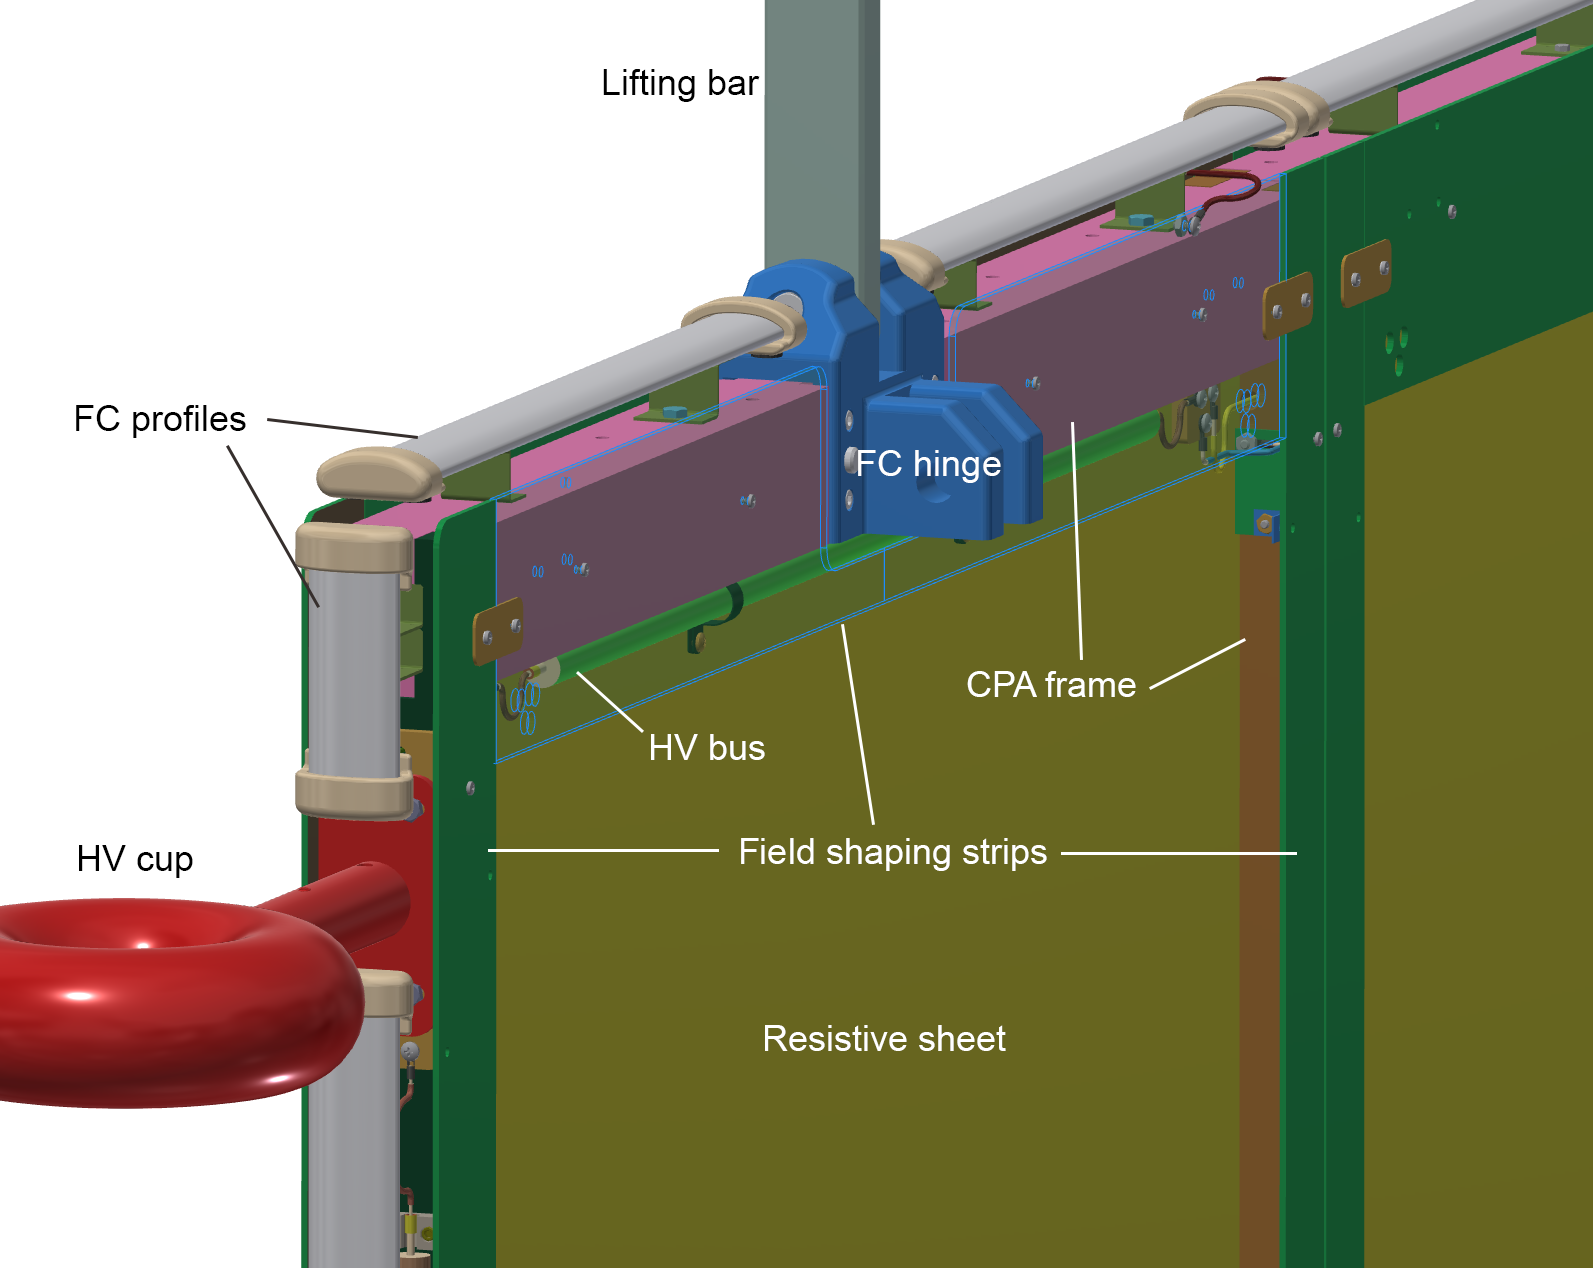
\includegraphics[width=0.6\textwidth]{donut_cpa2} %{ was Latest3D}
\end{dunefigure}

In accordance with specification SP-FD-17, 
the surface resistivity of the \dwords{rp} is required to be greater than \cathodemegohm to provide for slow reduction of accumulated charge in the event of a discharge.  Given the anticipated higher stored energy at the \dword{fd} 
relative to the prototypes, we set a goal of \cathodegigohm to further  protect against potential discharges.  
 
To maintain the position and flatness of the cathode, 
\SI{6}{cm} thick \frfour frames are placed at \SI{1.2}{m} intervals between the \dword{cpa} panels. This design ensures the cathode distortion caused by a small pressure differential (up to \SI{1}{Pa}) across the cathode surface from the convective flow of the \dword{lar} is less than \SI{1}{cm}, meeting the specification of less than \SI{3}{cm}, which causes a field uncertainty of 1\%.

The \dword{cpa} frames are required to support, in addition to the \dword{hv} components, the \dword{topfc} and \dword{botfc} units attached to both sides of the \dword{cpa} plane. The arrangement and deployment of these components is identical to that in \dword{pdsp}.  Figure~\ref{fig:cpa_panel-complete} shows a completed \dword{pdsp} \dword{cpa} panel on the production table ready for lifting into vertical position. % for mounting on its trolley.

\begin{dunefigure}[Completed ProtoDUNE-SP CPA panel on production table]{fig:cpa_panel-complete}{Completed \SI{6}{m} long \dword{pdsp} \dword{cpa}  panel on production table.  A \dword{cpa} plane is made up of two panels side-by-side.}
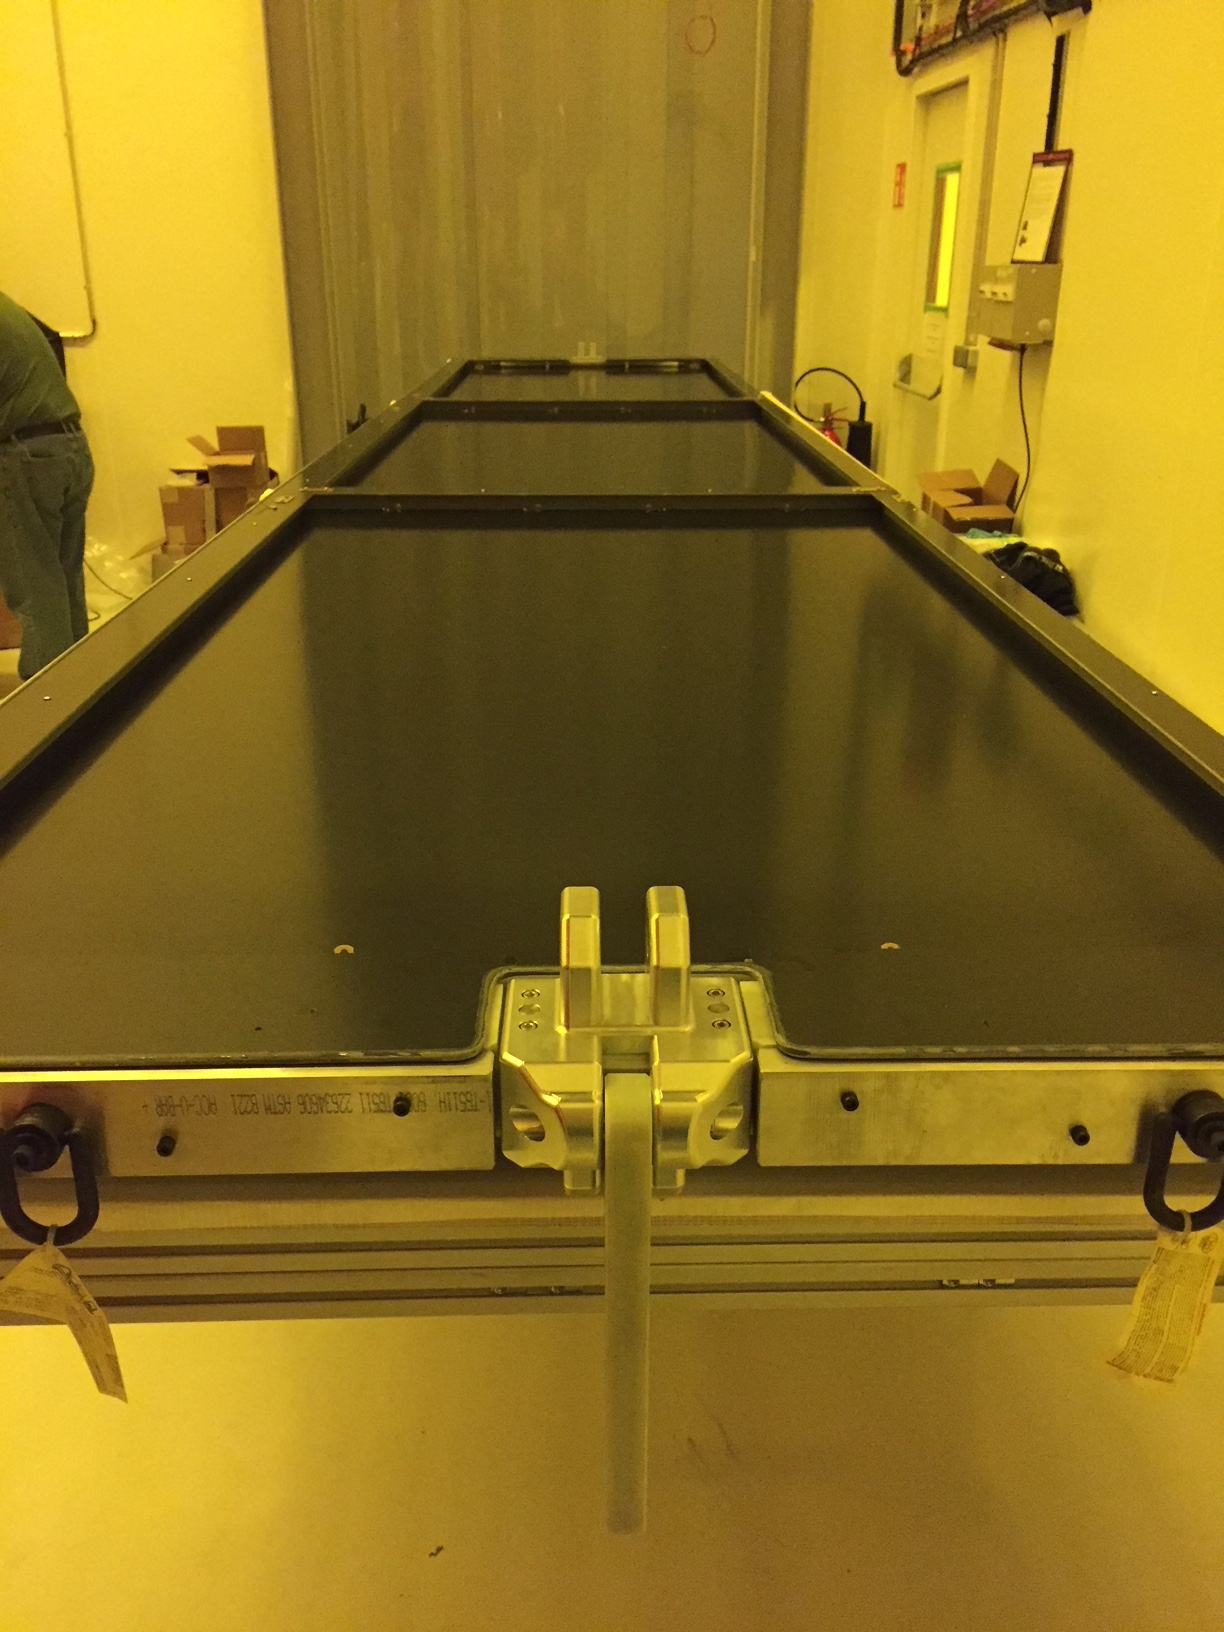
\includegraphics[width=0.7\textwidth]{cpa_panel-complete}
\end{dunefigure}

 Since \frfour is a good insulator at cryogenic temperatures with a dielectric constant different from that of \dword{lar}, the presence of the \dword{cpa} panel frames causes a local \efield distortion that can become pronounced if the frame surface becomes charged 
from ionization in the \dword{tpc}.  To minimize this distortion, resistive field-shaping strips (\dword{fss}) are placed on the frame and biased at a different potential.  Figure~\ref{fig:fss_concept} illustrates the drift field uniformity improvement with these strips.

\begin{dunefigure}[Benefit of field-shaping strip concept]{fig:fss_concept}{A comparison of three cathode cross sections to illustrate the benefit of the \dword{fss}. Both equipotential lines (horizontal) and \efield{} lines (vertical) are shown.  The amplitude of the \efield{} is shown as color contours. Each color contour is a 10\% step of the nominal drift field.  The gray rectangles represent the frame and the resistive sheet in each case. Left: a conductive/resistive frame similar to that of \dword{icarus} or \dword{sbnd}; Middle: an insulating frame with the insulating surfaces charged to an equilibrium state; Right: an insulating frame covered with \dword{fss} (purple) and biased at the optimum potential. }
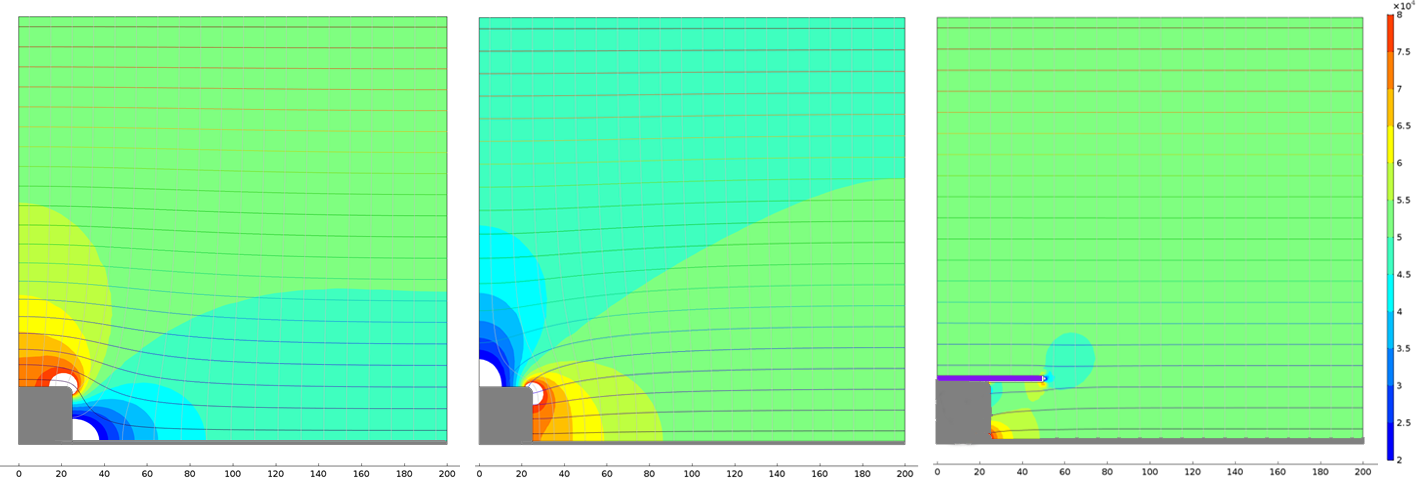
\includegraphics[width=0.95\textwidth]{field-shaping-strip-concept} %{ was Latest3D}
\end{dunefigure}

Other \dword{hv} components of the \dword{cpa} arrays include  edge aluminum profiles (to act as the first elements of the \dword{fc}) and cable segments forming the \dword{hv} bus. 

There are at least two instances of electrical connections on the \dword{cpa} array and between the \dword{cpa} array and other \dword{hv} system components (top, bottom, and \dwords{ewfc}), and four connections between \dwords{rp} in a \dword{cpa} unit.  Each of the different types of electrical connections on the \dword{cpa} were tested in a \dword{ln} tank at \dword{bnl}~\cite{bib:docdb2338}  and in \dword{pdsp}. %There were no failures at BNL and none at \dword{pdsp}.  
No failures occurred at either \dword{bnl} or \dword{pdsp}. The \dword{hv} connection from the \dword{hv} power supply is a closed loop around the \dword{cpa} that can sustain at least one broken connection without loss of the cathode \dword{hv}.  This ensures compliance with requirement~\ref{ spec:hv-connection-redundancy }.

Visual inspection of these items during the assembly process is done to ensure that no accidental sharp points or edges have been introduced. The surface resistivity of the \dword{cpa} \dwords{rp} and the \dword{fss} are checked multiple times during assembly, first when the resistive panels and strips are received and after assembly into \dword{cpa} units on the table.  Coated parts that do not meet the minimum surface resistivity requirement are replaced.  This ensures that requirement SP-FD-17 is satisfied. No discharges were observed in \dword{protodune}, so no additional cryogenic tests are planned for the \dword{cpa}s for DUNE. 



%%%%%%%%%%%%%%%%%%%%%%%%%%%%
\section{Field Cage}
\label{sec:fdsp-hv-des-fc}


The \dword{fc} is introduced in Section~\ref{subsec:fdsp-hv-des-fc}. Its function, basic characteristics, and components are described there. 
The \dword{fc} %have been 
is designed to %ensure they 
meet the system specifications listed in Section~\ref{sec:fdsp-hv-des-consid}. %Table~\ref{tab:hvphysicsreqs}. 
To allow the system to reach the design \efield{} uniformity 
(specification SP-FD-11), 
%(specification~\ref{tab:spec:hvs-field-uniformity}) %(requirement 1) 
all components other than the aluminum profiles, \dwords{gp}, and electronic divider boards are made of insulating \dword{frp} and \frfour materials, and the end of each profile is covered with a \dword{uhmwpe} end cap. \\

All voltage divider boards provide redundancy for establishing the profile-to-profile potential differences with only minor distortions to the \efield in case of failure of any individual part, and two redundant boards provide the connection from the \dwords{fc} modules to the \dword{cpa} 
(specification \ref{ spec:hv-connection-redundancy }).  
The aluminum profiles are attached to \dword{frp} pultruded structural elements, including I-beams and box beams.  
Pultruded \dword{frp} material is non-conductive and strong enough to withstand the \dword{fc} loads  in the temperature range of \SI{-150}{C} and \SI{23}{C}, as certified by vendors. Testing of the \dword{frp} joints were conducted at \dword{ln} temperatures~\cite{bib:docdb1504}. 
The material was stronger at these temperatures than at room temperature, 
providing confidence in the material behavior at \dword{lar}  temperature. The \dword{frp} material meets class A standards for fire and smoke development established by the International Building Code characterized by ASTM E84.\footnote{ASTM E84-20, Standard Test Method for Surface Burning Characteristics of Building Materials, ASTM International, West Conshohocken, PA, 2020, \url{https://www.astm.org}.}

The top and bottom \dwords{fc} %modules 
are supported by the \dword{cpa} and \dword{apa} arrays. The \dword{ewfc} modules, 
\SI{1.5}{\m} tall by \SI{3.5}{\m} long, are stacked eight units high (\SI{12}{\m}) and are supported by the installation rails above the \dword{cpa} and \dword{apa} arrays.



%%%%%%%%%%%%%%%
\subsection{Field Cage Profiles}
\label{sec:fdsp-hv-des-fc-profiles}

The \dword{fc} consists of modules of extruded aluminum  field-shaping  %electrodes (
profiles, as listed in Table~\ref{tab:fcparts}. The shape of these %electrodes 
profiles is chosen to minimize the strength of the \efield{} between a given profile and its neighbors and between a profile and
other surrounding parts, including the \dword{gp}. For example, with a \SI{30}{\cm} separation between the \dword{fc} and the \dword{gp}, the maximum \efield{} on the profiles surface is under \SI{10}{\kilo\volt\per\centi\meter} over the straight sections of the profiles at \SI{-180}{\kV} bias (Figure~\ref{fig:profile-e-field}).  


\begin{dunefigure}
[\efield{} map and equipotential contours of profiles at \SI{-180}{\kV}]
{fig:profile-e-field}
{\efield{} map (color) and equipotential contours of an array of the \dword{fc} profiles biased up to \SI{-180}{\kV} and a ground clearance of \SI{30}{\cm}.} %(Credit: BNL CAD model).} 
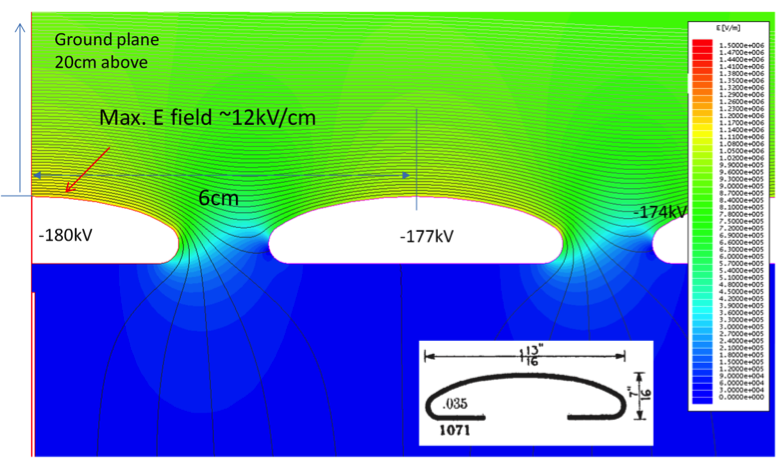
\includegraphics[width=0.8\textwidth]{profile-e-field.png}
\end{dunefigure}

The profile ends have higher surface \efield{}, especially those at the corners of the \dword{fc}. To prevent high voltage breakdown in the \dword{lar}, the ends of the profiles are encapsulated by custom \dword{uhmwpe} caps.  These caps are designed and experimentally verified to withstand the full voltage across their \SI{6}{\milli\m} thickness. 

The profiles and their end caps have been carefully modeled to ensure the resulting \efield{}
 does not approach \SI{30}{\kV}/{cm}~\cite{Blatter:2014wua} (specification SP-FD-24). This design concept was validated in a small-scale test setup at \dword{cern} before it was adapted for the \dword{spmod}.  
These features are designed to avoid sparking and thus to draw very small stable currents, 
which should produce a consistent load on the power supply 
(specifications~\ref{ spec:hv-ps-ripple }, \ref{ spec:cathode-resistivity }, 
and~\ref{ spec:power-supply-stability }. % SP-FD-12, SP-FD-17, and SP-HV-1).


%%%%%%%%%%%%%%%
\subsection{Ground Planes}
\label{sec:fdsp-hv-des-fc-gp}

For safe and stable operation of the \dword{lar} cryogenics system, the cryostat requires a small fraction of its volume to be filled with gaseous argon. This small volume is commonly referred to as the ullage. To optimize use of the \dword{lar} in the cryostat, we will place the upper \dword{fc}, which forms the top boundary of the \dword{tpc}, just below the liquid surface.

The ullage contains many grounded %metallic 
conducting components with sharp features, near which the \efield could easily exceed the breakdown strength of gaseous argon if directly exposed to the upper \dword{fc}. % below. 
To shield the high \efield from entering the gas ullage and thereby prevent such breakdowns, % in the argon gas, 
\dfirsts{gp}, %is added above the upper \dword{fc} electrodes at a safe distance but still below the liquid surface.  
in the form of tiled, perforated stainless steel sheet panels, are mounted on the outside surface of the 
\dword{topfc} module with a \SI{30}{cm} clearance. While critical over the region near the cathode, the need for such shielding diminishes toward the \dword{apa} end of the \dword{fc} due to the lower voltages on the \dword{fc} profiles in that region. 
The 30\,cm \dword{fc}-\dword{gp} distance represents a 50\% increase over the value used in \dword{pdsp}, to further reduce the maximum \efield in the \dword{tpc} and thus the possibility of discharges. The 20\,cm distance in \dword{pdsp} was due to an early DUNE design, where 20\,cm was the maximum possible distance that could maintain the \dword{gp} below the liquid level. With the current cryostat and \dword{spmod} design, more space is available, allowing an increase in the \dword{fc}-to-\dword{gp} distance. 
 
In addition to the increase in \dword{fc} to \dword{gp} clearance, we are also eliminating most of the insulating standoffs used in \dword{pdsp} that support \dword{gp} tiles from the \dword{fc} I-beams, in particular, those near the \dword{cpa} end of the \dword{fc}.  These standoffs  are deemed at risk of aiding discharges by providing a short path from \dword{fc} to \dword{gp} along corresponding straight edges.  Figure~\ref{fig:new-fc} illustrates the new configuration. Figure~\ref{fig:new-fc_mockup} shows a test stand built to demonstrate the coupling between \dword{fc} and \dword{gp}, with the standoffs near the cathode end removed. Tests in \dword{ashriver} are confirming that no changes in the assembly or deploying procedures are needed and that the mechanical stability of the full system is unaffected. An upcoming review will examine the design changes and related tests and calculations. Final validation of the complete \dword{hv} design for the \dword{spmod} will be performed in future \dword{protodune} running.


\begin{dunefigure}
[Current baseline FC+GP module design; changes relative to ProtoDUNE-SP]
{fig:new-fc}
{Comparison between the \dword{fd} \dword{topfc} module (top) and the \dword{pdsp} counterpart (bottom).  The changes to the \dword{cpa} side standoffs in the \dword{fd} version are highlighted in red circles.  The increase in the \dword{fc} to \dword{gp} separation is also shown here.} 
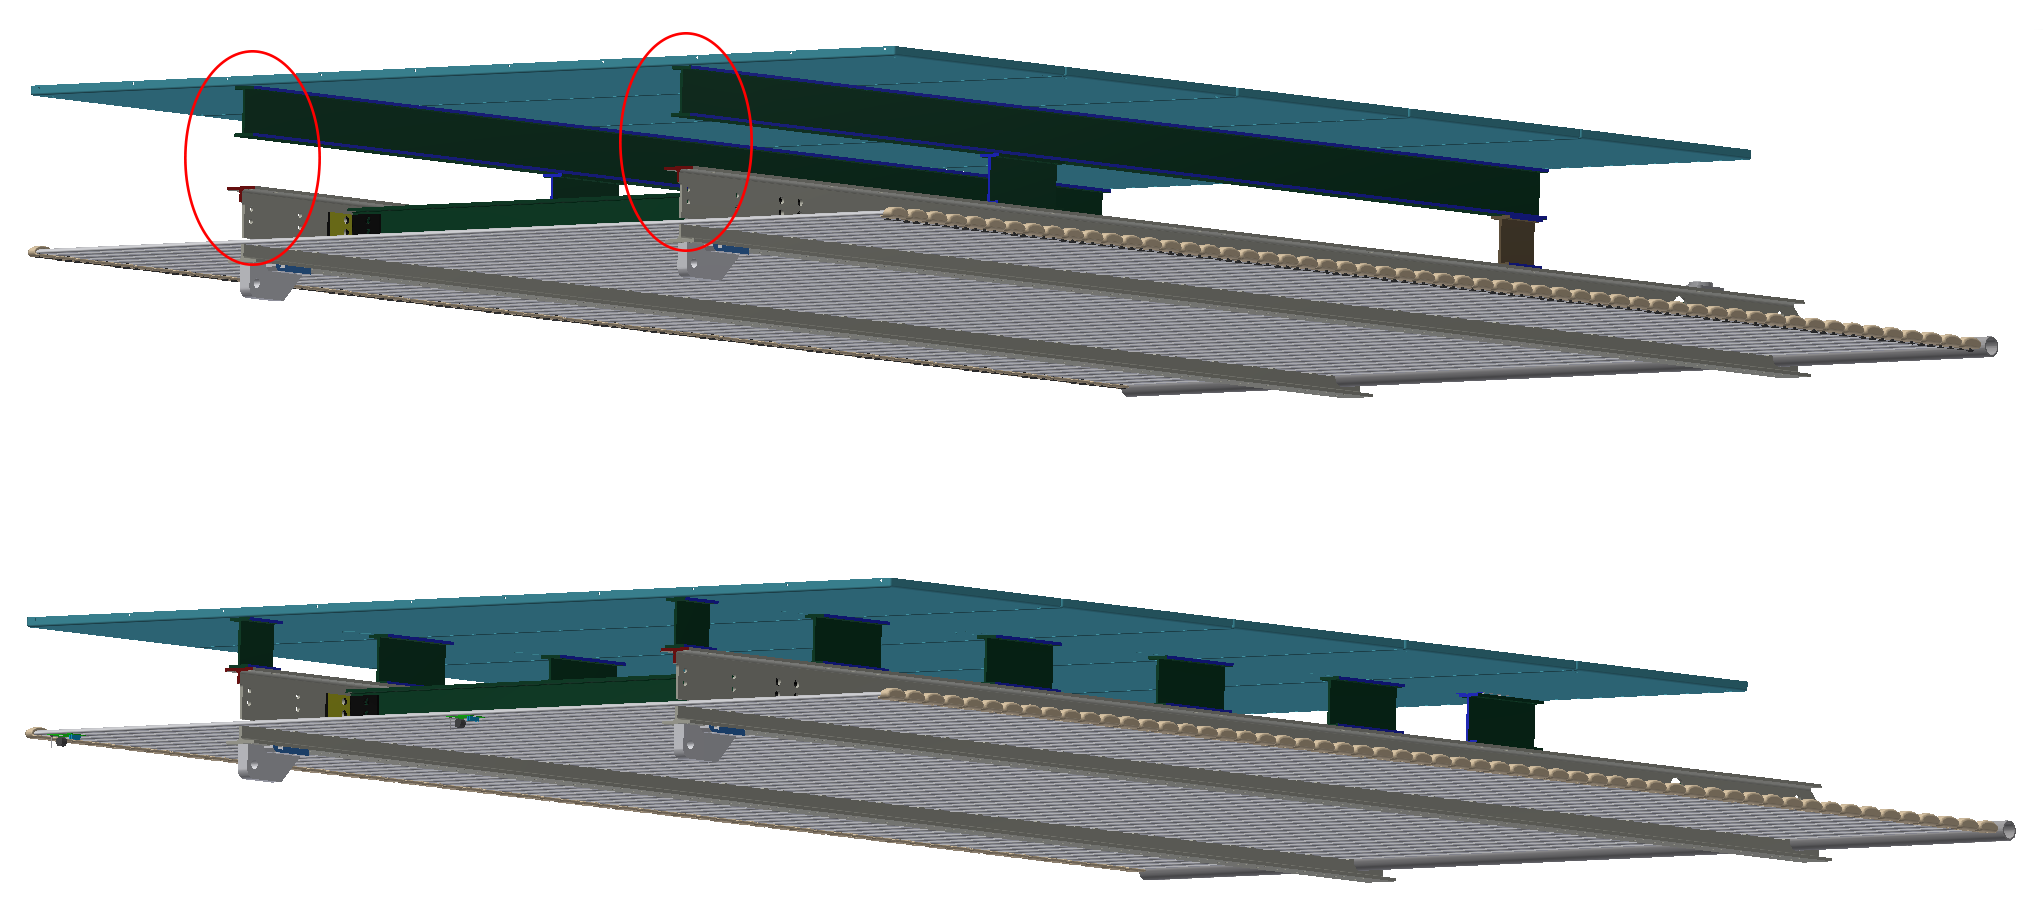
\includegraphics[width=0.9\textwidth]{TBFC_FD_vs_PD.png}
\end{dunefigure}

\begin{dunefigure}
[Coupling between \dshort{fc} and \dshort{gp}]
{fig:new-fc_mockup}
{Photos of a test module demonstrating the coupling between the  \dword{fc} and \dword{gp}, with the standoffs near the cathode end (towards the right) removed.} %(Credit: Univ. of Minnesota).}%
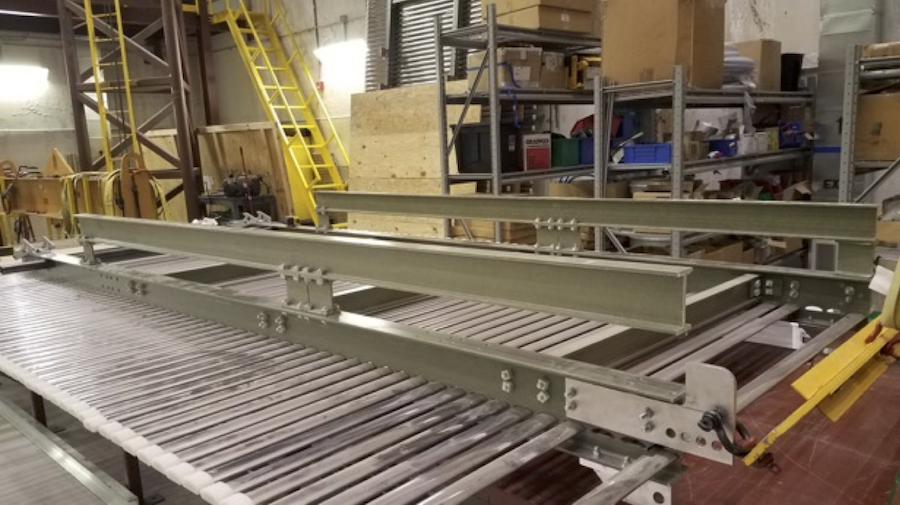
\includegraphics[width=0.48\textwidth]{FC_mockup-1.png}
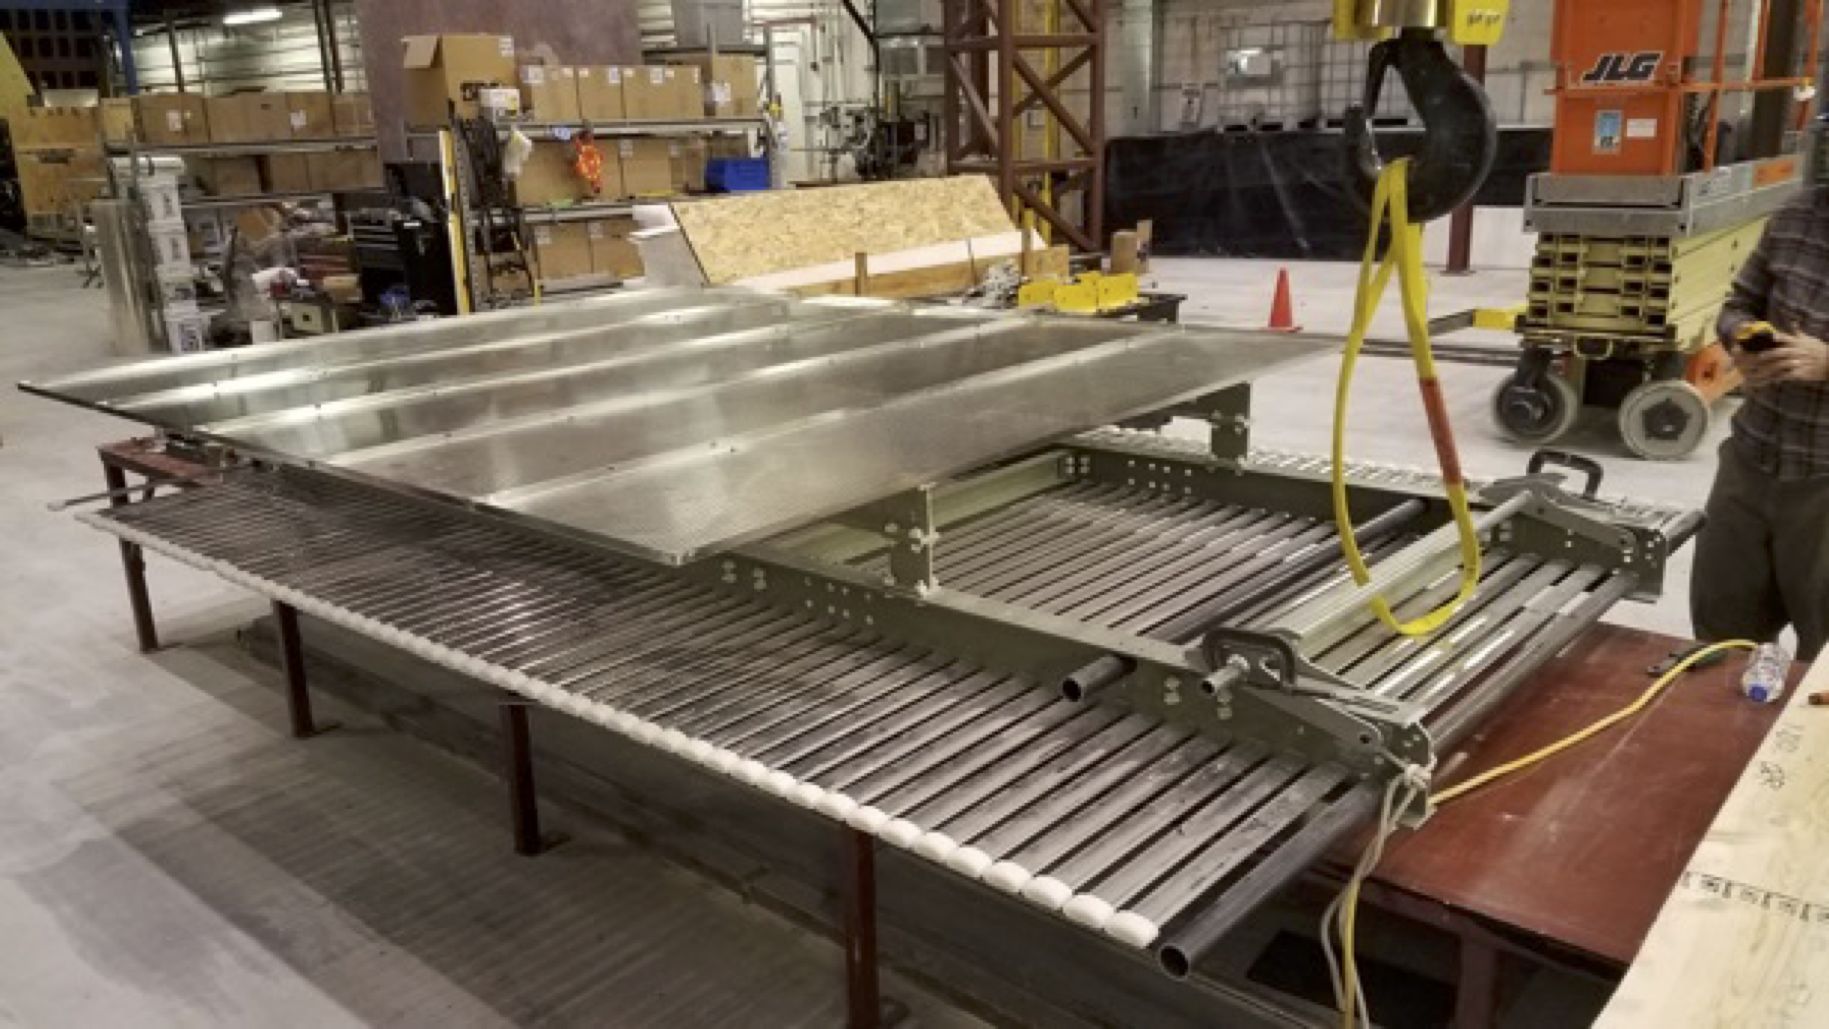
\includegraphics[width=0.48\textwidth]{FC_mockup-2.png}
\end{dunefigure}

On the bottom of the cryostat a similar set of \dwords{gp} %is planned to 
will protect against %prevent 
breakdown in the liquid near cryogenic pipings and other sensors with sharp features. The same clearance will be used. No \dwords{gp} are planned beyond the two \dwords{ewfc} since there is sufficient clearance in those regions.  


%%%%%%%%%%%%%%%
\subsection{Maximum Field Distortions}
\label{sec:fdsp-hv-des-fc-mfd}

The \dwords{fc} are designed to produce a uniform \efield with understood characteristics.
The largest known \efield distortion in the \dword{tpc} occurs around a large gap in the \dword{fc} between the endwall module and its neighboring top and bottom modules. This gap is necessary to allow the top and bottom modules to rotate past the \dword{ewfc} during deployment.  Figure~\ref{fig:fc-distortion} illustrates the extent of the distortion in this limiting scenario. 
%If this feature remains
In the \dword{spmod}, a total \dword{lar} mass of \SI{160}{kg} along these four edges of the \dword{tpc} suffers $>\,\SI{5}{\%}$ \efield distortions.  If the non-uniformity is not accounted for in reconstruction, this will result in uncertainties in $dE/dx$ in these regions exceeding 1\%. 

\begin{dunefigure}[\efield at edge of field cage]
{fig:fc-distortion}
{\efield at a corner between the bottom and endwall \dword{fc} modules, showing effects of a \SI{7}{cm} gap. Left: the extent of \num{5}\% \efield{} non-uniformity boundary (black surface, contains less than \SI{10}{kg} of \dword{lar}) and \num{10}\% non-uniformity boundary (white surface, contains $\sim$\SI{6}{kg} of \dword{lar}) inside the \dword{tpc}'s active volume. The inset is a view from the CAD model.  Right: electron drift lines originating from the cathode surface.}
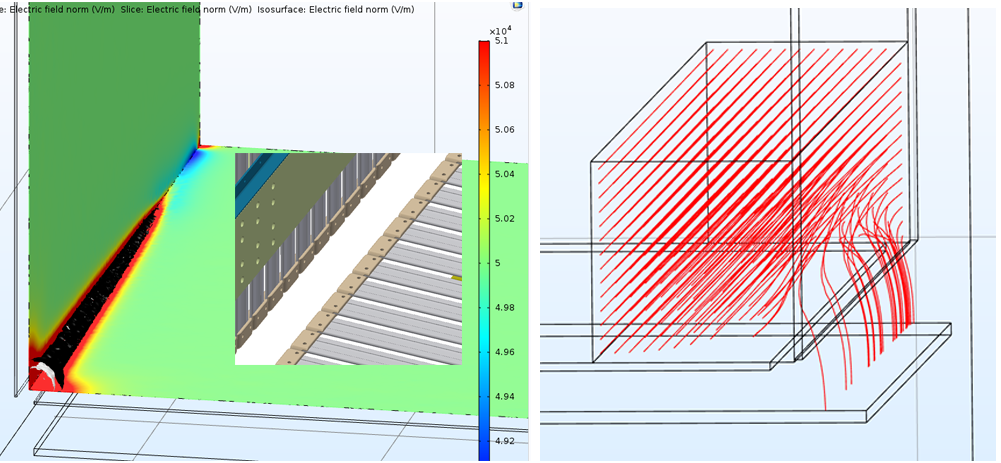
\includegraphics[width=0.9\textwidth]{distortion_from_fc_gap}
\end{dunefigure}



%%%%%%%%%%%%%%%%%%%%%%%%%%%
\subsection{Top and Bottom Field Cage Modules}
\label{sec:fdsp-hv-des-fc-tbmods}

The \dword{topfc} and \dword{botfc} module dimensions are listed in Table~\ref{tab:fcparts}. The length, \spfcmodlen{}, is set by the length of the two \SI{15.2}{\cm} (\SI{6}\,in) \dword{frp} I-beams that form the primary support structure of the modules. The I-beams are connected to each other by three  \SI{7.6}{\cm} (\SI{3}\,in) \dword{frp} cross beams. The connections between the longitudinal and cross I-beams are made with L-shaped \dword{frp} braces that are attached to the I-beams with \dword{frp} spacer tubes, and secured with \dword{frp} threaded rods, \dword{frp} hex-head nuts, and custom-machined \frfour washer plates.

The \SI{2.3}{\m} module width corresponds to the length of the aluminum profiles, including the UHMW polyethylene end caps. Profiles are secured to the \dword{frp} frame using custom-machined double-holed stainless steel slip nuts that are slid into and electrically in direct contact with the aluminum profiles such that they straddle the webbing of the \SI{15}{\cm} I-beams, and are held in place with screws that penetrate the I-beam flanges. The profile offset with respect to the \dword{frp} frame is different for modules closest to the \dwords{ewfc}, %endwalls, 
and modules in the center of the active volume.

Five \dwords{gp} are connected to the outside (i.e., the non-drift side) of each \dword{topfc} and \dword{botfc} module. The \dwords{gp} are positioned $\sim$\SI{30}{\cm} away from the profiles, and begin at the \dword{cpa} end of the module, leaving the last 14 profiles (\SI{88}{\cm}) on the \dword{apa} end of the module exposed. Between the \dwords{gp} and the \SI{15}{\cm} I-beams standoffs made of short sections of \SI{10.2}{\cm} (4\,in)  \dword{frp} I-beams are connected with \dword{frp} threaded rods and slip nuts. The electrical connection between the \dwords{gp} is made with copper strips.

The connections between the top and bottom modules and the \dword{cpa}s are made with aluminum hinges, \SI{2.54}{\cm} (1\,in) in thickness, that allow the modules to be folded in on the \dword{cpa} during installation. The hinges are electrically connected to the second profile from the \dword{cpa}. The connections to the \dword{apa}s are made with stainless steel latches that are engaged once the top and bottom \dword{fc} modules are unfolded and fully extended toward the \dword{apa}.

The voltage drop between adjacent profiles is established by voltage divider boards screwed into the drift-volume side of the profiles. A custom-machined nut plate %is used that can be 
is inserted into the open slot of each profile and twisted \SI{90}{\degree} %$^\circ$ 
to lock into position. Two additional boards to connect the modules to the \dword{cpa}s %were screwed 
screw into the last profile on the \dword{cpa} end of the module. This system is %also 
more fully described in Section~\ref{sec:fdsp-hv-design-interconnect}. A fully assembled module is pictured in Figure~\ref{fig:tbfc1-2}.

\begin{dunefigure}[Fully assembled \dshort{topfc} module with \dshort{gp}]{fig:tbfc1-2}{A fully assembled \dfirst{topfc} module with \dfirst{gp} is shown.} %as well as a closeup of a \dword{cpa} end as viewed from the bottom (drift) side of the module.}
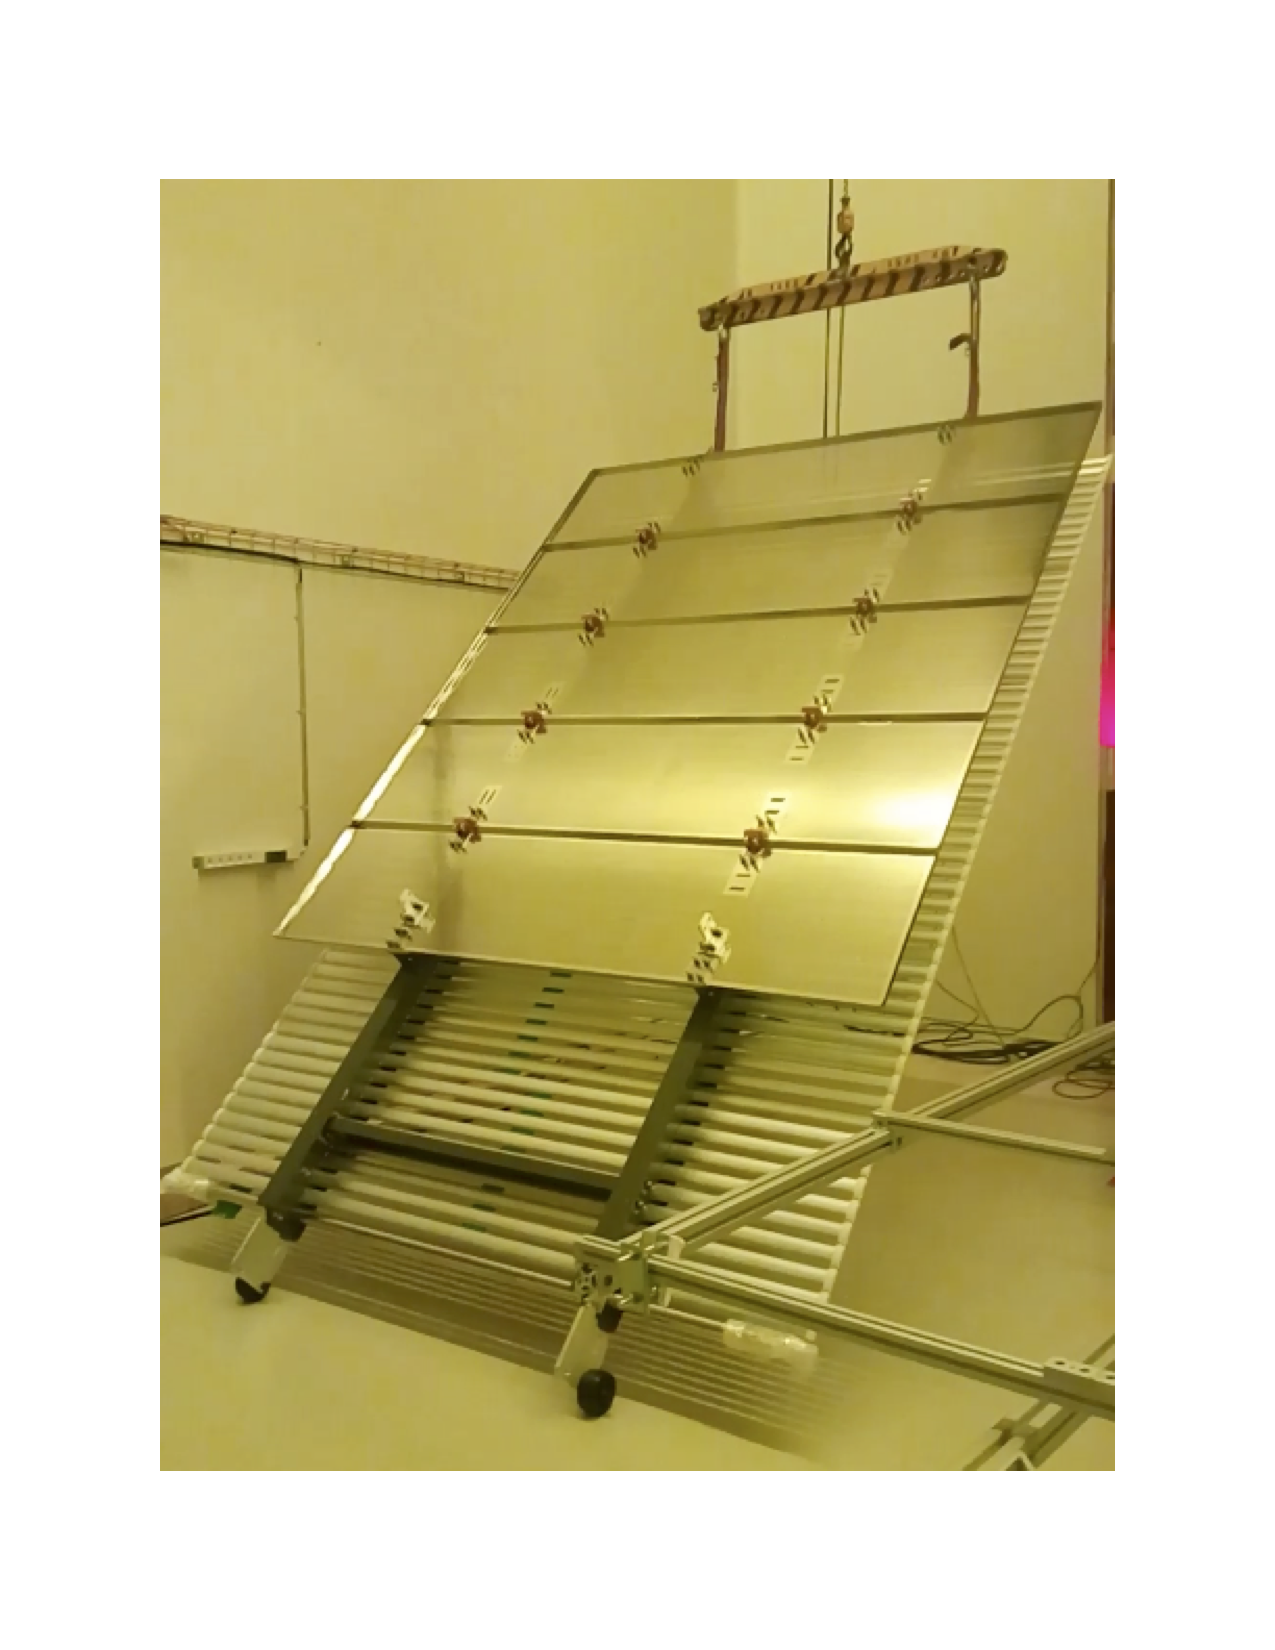
\includegraphics[width=0.45\textwidth]{FC_with_GP}
%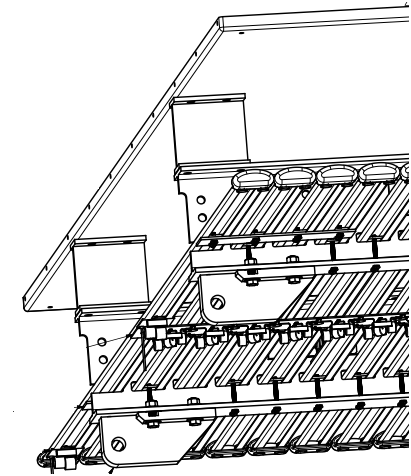
\includegraphics[width=0.33\textwidth]{tbfc2}
\end{dunefigure}


\subsection{Endwall Field Cages (EWFC)}
\label{sec:fdsp-hv-des-fc-ewfc}


Each of the four drift volumes has two \dwords{ewfc}, one on each end. Each \dword{ewfc} is in turn composed of eight \dword{ewfc} modules.  The two endwalls are identical in construction, and are installed with an 180$^\circ$ rotation front to back.
Figure~\ref{fig:fc_endwall_panels} illustrates the layout for the topmost 
and the other panels, respectively.



Each \dword{ewfc} module is constructed of two \dword{frp} box beams, each \SI{3.5}{\m} long, as shown in \ref{fig:fc_endwall_panels}. 
The box beam design also incorporates cutouts on the outside face to minimize charge build up. Box beams are connected using \SI{1.27}{\cm} (\num{0.5}\,in) thick \dword{frp} plates. The plates are connected to the box beams using a shear pin and bolt arrangement. The inside plates facing the active volume are connected using special stainless steel slip nuts and stainless steel bolts. The field-shaping profiles are connected to the top box beam using stainless steel slip nuts, an \dword{frp} angle, and two screws each that pass through matching holes in the wings of the aluminum profiles. At the bottom box beam, the profiles are pulled against another \dword{frp} angle with a single screw and a slip nut that is held in place by friction.

\begin{dunefigure}[Endwall FC panels]{fig:fc_endwall_panels}{Top: Uppermost module of the \dword{ewfc}. The two G10 hanger plates connect the \dword{ewfc} to the \dword{dss} beams above the \dword{apa}s and \dword{cpa}s. Bottom: regular \dword{ewfc} module. Seven such modules stack vertically with the top module to form the \SI{12}{m} total height.}
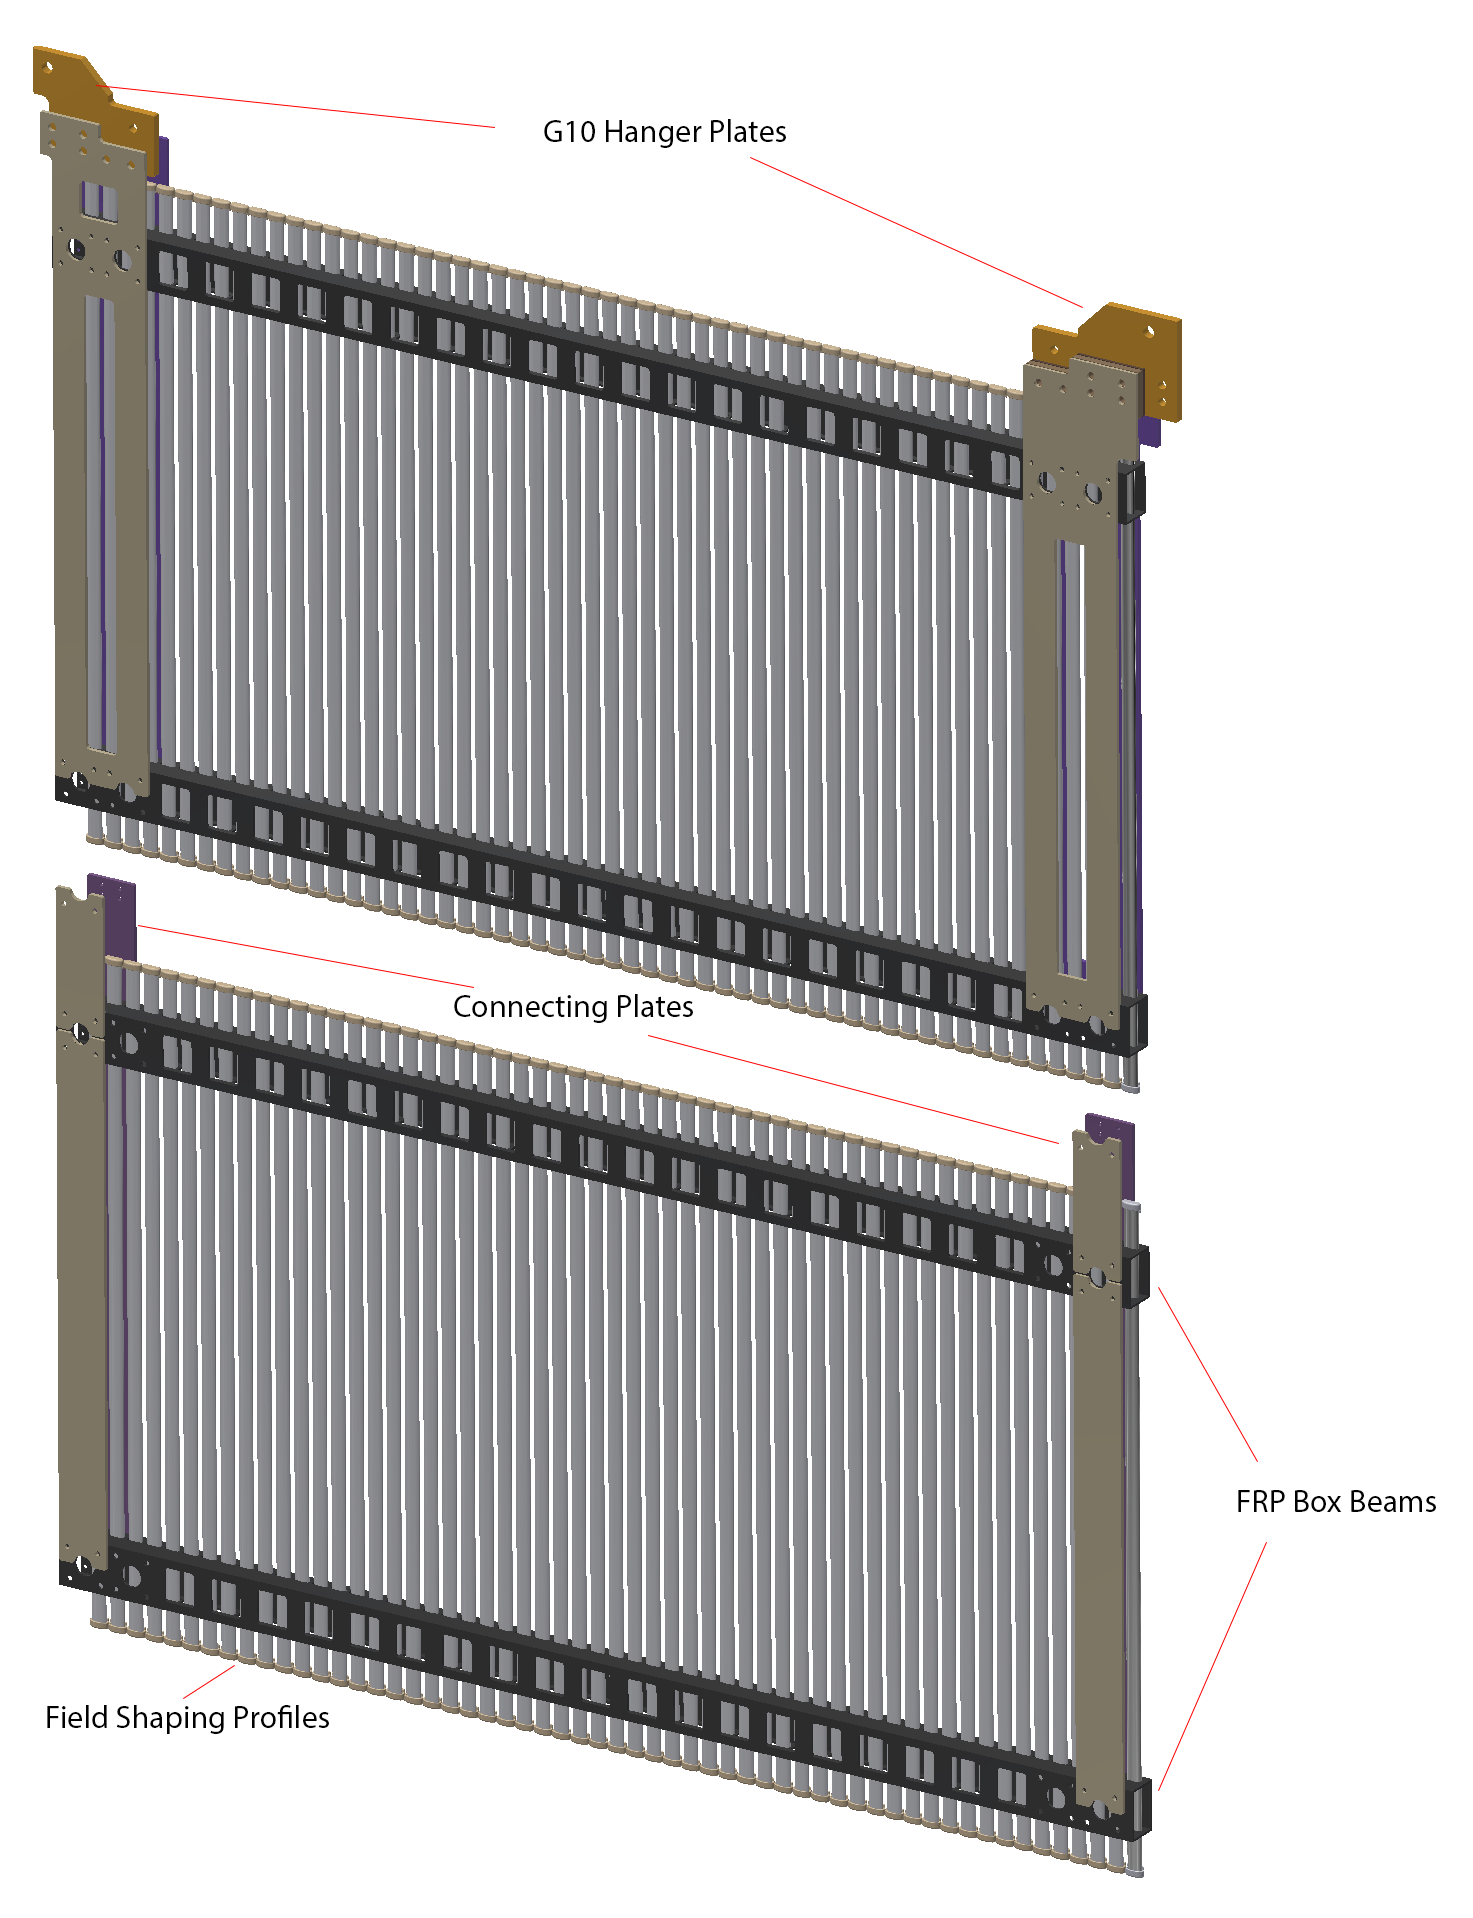
\includegraphics[width=0.8\textwidth]{EWFC_modules.png}
\end{dunefigure}



\subsection{Voltage Divider Boards}
\label{sec:fdsp-hv-des-fc-vdb}

A resistive divider chain interconnects all the metal profiles of each \dword{fc} module to provide a linear voltage gradient between the cathode and anode planes.

The resistive divider chain is %realized with 
 a chain of resistor divider boards each with %hosting 
eight resistive stages in series. 
 Each stage (corresponding to \SI{6}{cm} gap between \dword{fc} profiles) consists of two \SI{5}{\giga\ohm} resistors in parallel yielding a parallel resistance of \SI{2.5}{\giga\ohm} per stage to hold a nominal voltage difference of \SI{3}{kV}. Each stage is protected against high voltage discharge transients by transient/surge absorbers (varistors). To achieve the desired clamping voltage, three varistors (with \SI{1.8}{kV} clamping voltage) are wired in series and placed in parallel with the associated resistors. A schematic of the resistor divider board is shown in Figure~\ref{fig:ResDivBoa}; an illustration of the resistor divider board used in \dword{pdsp} is shown as well.
These boards will be identical to the ones successfully mounted in the \dword{pdsp} \dword{fc}. 

\begin{dunefigure}[ProtoDUNE-SP HV resistor divider board]{fig:ResDivBoa}
  {Left: A \dword{pdsp} resistor divider board. Right: Schematic diagram of resistor divider board}
  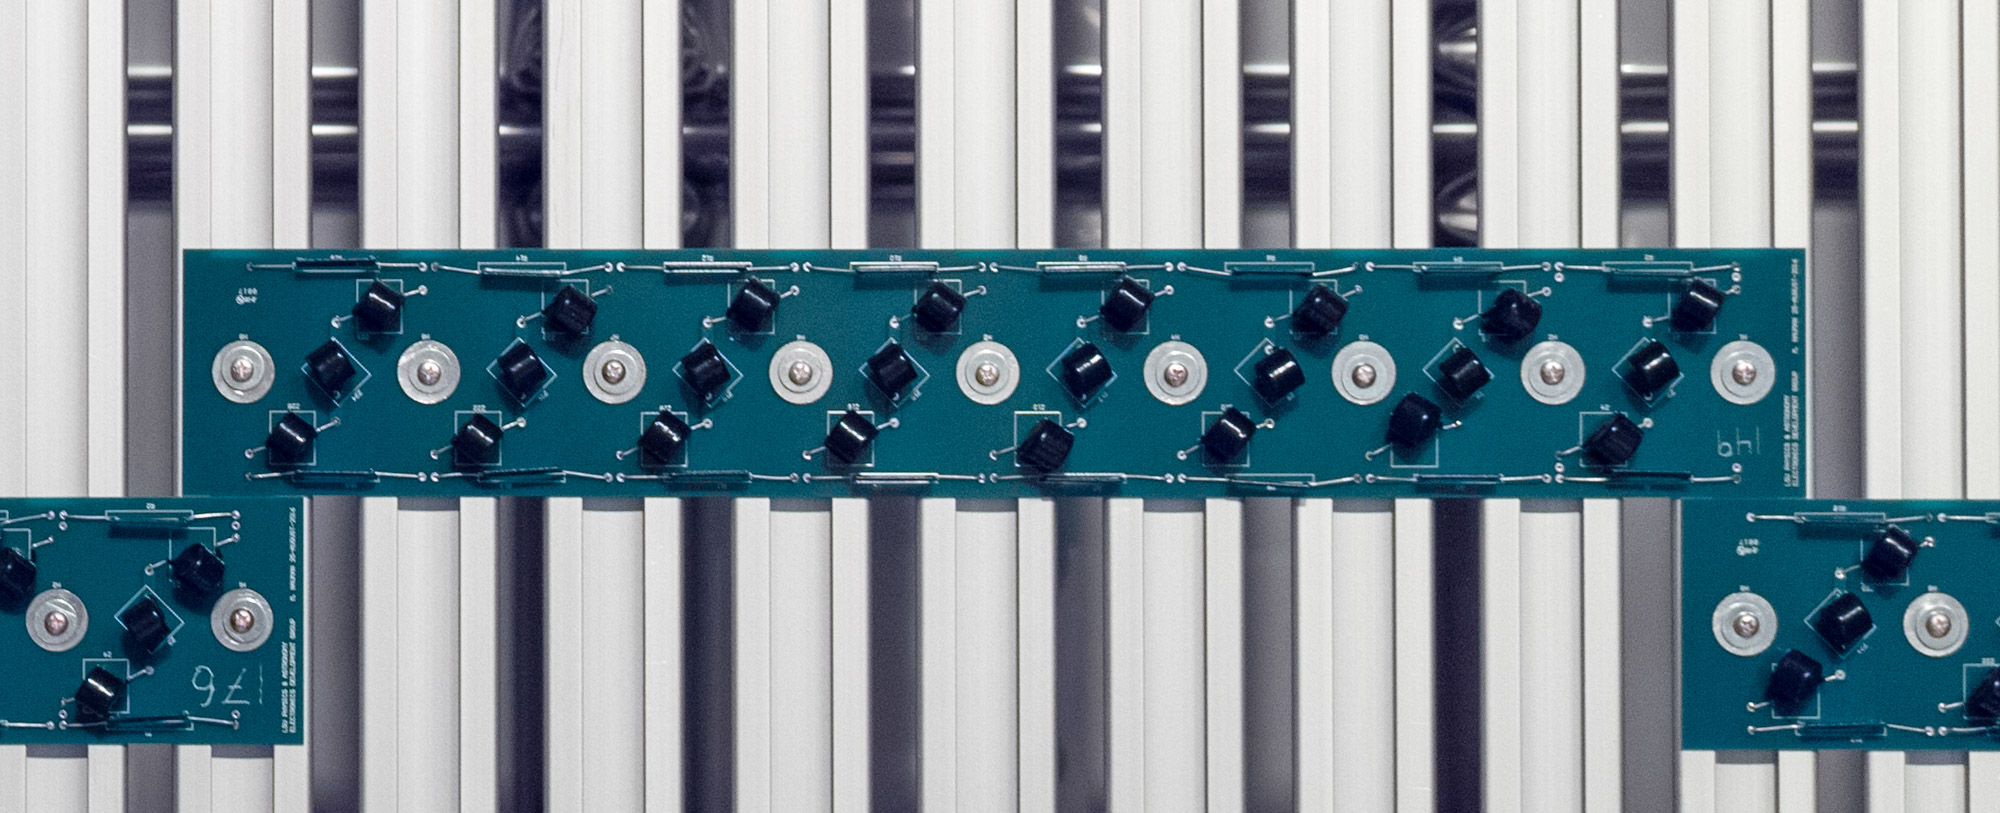
\includegraphics[width=0.48\textwidth]{Divider_board.jpg}
  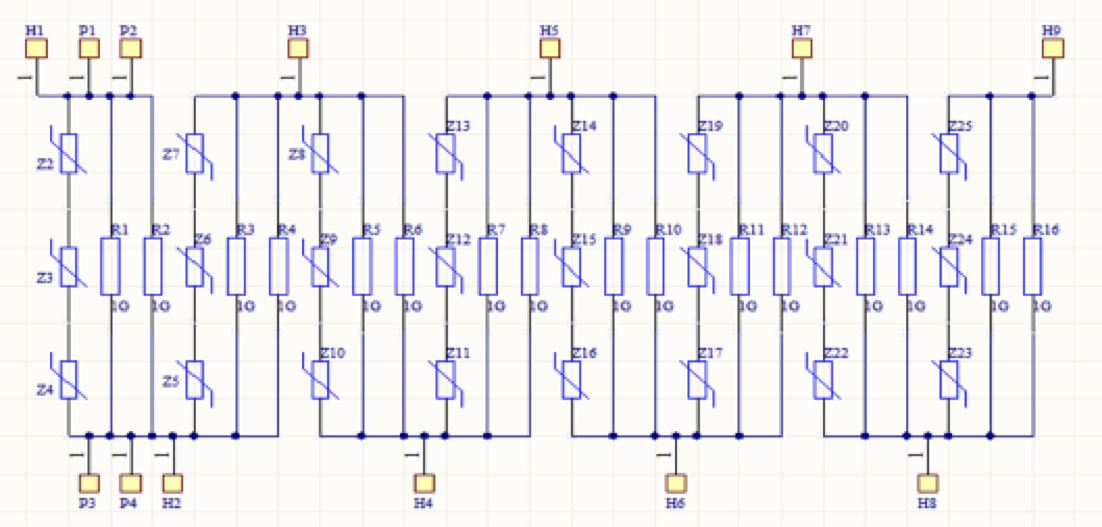
\includegraphics[width=0.48\textwidth]{ResDivBoa.png}
\end{dunefigure}


The current drawn by each divider chain is about $1.2~\mu A$ at the nominal \efield{} of \SI{500}{V/cm}. A total of 132 resistive divider 
boards are connected in parallel to each \dword{cpa} array for a total of about $158~\mu A$, well within the capability of the selected \dword{hv} power supply.

There are about 30,000 resistors used on the \dwords{fc} in an \dword{spmod}. A resistor failure is a possible risk to the \dword{tpc}.  
An open resistor on the divider chain, the most common failure mode, would approximately double the voltage across the remaining resistor to \SI{6}{kV}.  This larger voltage would force the three varistors in parallel to that resistor into conduction mode, resulting in a voltage drop of roughly \SI{5}{kV} (\SI{1.7}{kV} $\times$ \num{3}), while the rest of the divider chain remains linear, with a slightly lower voltage gradient. 
Because the damage to the divider would be local to one module, its impact to the \dword{tpc} drift field is limited to region near this module, a benefit of the modular \dword{fc} design.
An example of a simulated \efield{} distortion that would be caused by a failed resistor is shown in Figure~\ref{fig:fc-broken-resistor}. 

\begin{dunefigure}[\efield distortion from broken voltage divider path]{fig:fc-broken-resistor}{Simulated \efield{} distortion from one broken resistor in the middle of the voltage divider chain on one \dword{botfc} module.The benefit of the redundancy scheme is emphasized by the limited extent of the \efield distortions. Left: Extent of \efield{} non-uniformity in the active volume of the \dword{tpc}. The green planes mark the boundaries of the active volume inside the \dword{fc}. The partial contour surfaces represent the volume boundaries where \efield{} exceeds 5\% (dark red, contains less than \SI{100}{kg} of \dword{lar}) and 10\% (dark blue, contains less than \SI{20}{kg} of \dword{lar}) of the nominal drift field. The units are \si{\volt\per\m} in the legend. Right: electron drift lines connecting the \dword{cpa} to \dword{apa} in a %bottom/end wall field cage 
\dword{botfc} corner.  The maximum distortion to the field line is about \SI{5}{cm} for electrons starting at mid-drift at the bottom edge of the active volume.}
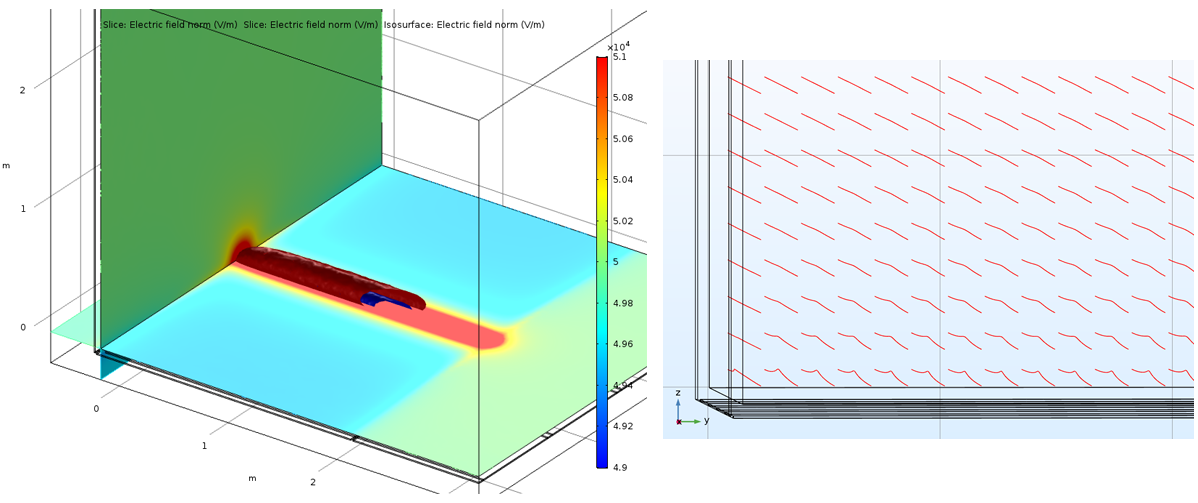
\includegraphics[width=0.9\textwidth]{e-field-distortion-due-to-open-resistor}
\end{dunefigure}
The effect of the non-uniformity in resistor values can also be scaled from this study.  A 2\% change in a resistor value (1\% change from the 2R in parallel) would give about 1.5\% of the distortion from a broken resistor, i.e. less than 1\,mm of transverse distortion in track position, with no noticeable drift field amplitude change inside the active volume.
 
%%%%%%%%%%%%%%%%%%%%%%%%%%%%
\section{Electrical Interconnections} % (Glenn)
\label{sec:fdsp-hv-design-interconnect}

Electrical interconnections are needed among the \dword{hv} delivery system, \dword{cpa} panels, \dword{fc} modules, and termination
boards on the \dword{apa} modules, as well as between resistive dividers and
the field-forming elements on the \dword{cpa}s and \dwords{fc}.  
Redundancy is
needed to avoid single points of failure. 
Some connections must be
insulated in order to avoid creating a discharge path that might
circumvent the discharge mitigation provided by the resistive \dword{cpa}
surface and \dword{fc} partitioning.  Certain connections must be
flexible in order to allow for \dword{fc} deployment, thermal
contraction, and motion between separately supported \dword{cpa}s components.  Figure~\ref{fig:fdsp-hv-design-interconnect-concept} shows a high-level
overview of the interconnections between the \dword{hv}, \dword{cpa}, and \dword{fc} modules.

\begin{dunefigure}[HV interconnection topology]{fig:fdsp-hv-design-interconnect-concept}
  {High-level topology of the \dword{hv} interconnections for one CPA array and adjacent field cages. Each pair of adjacent CPA panels is connected to two top field cage modules and two bottom field cage modules. A high voltage bus supplies the CPA panels at the top and bottom, and also supplies the endwall field cage modules. All field cages are terminated at the \dword{apa}s (not shown).}
  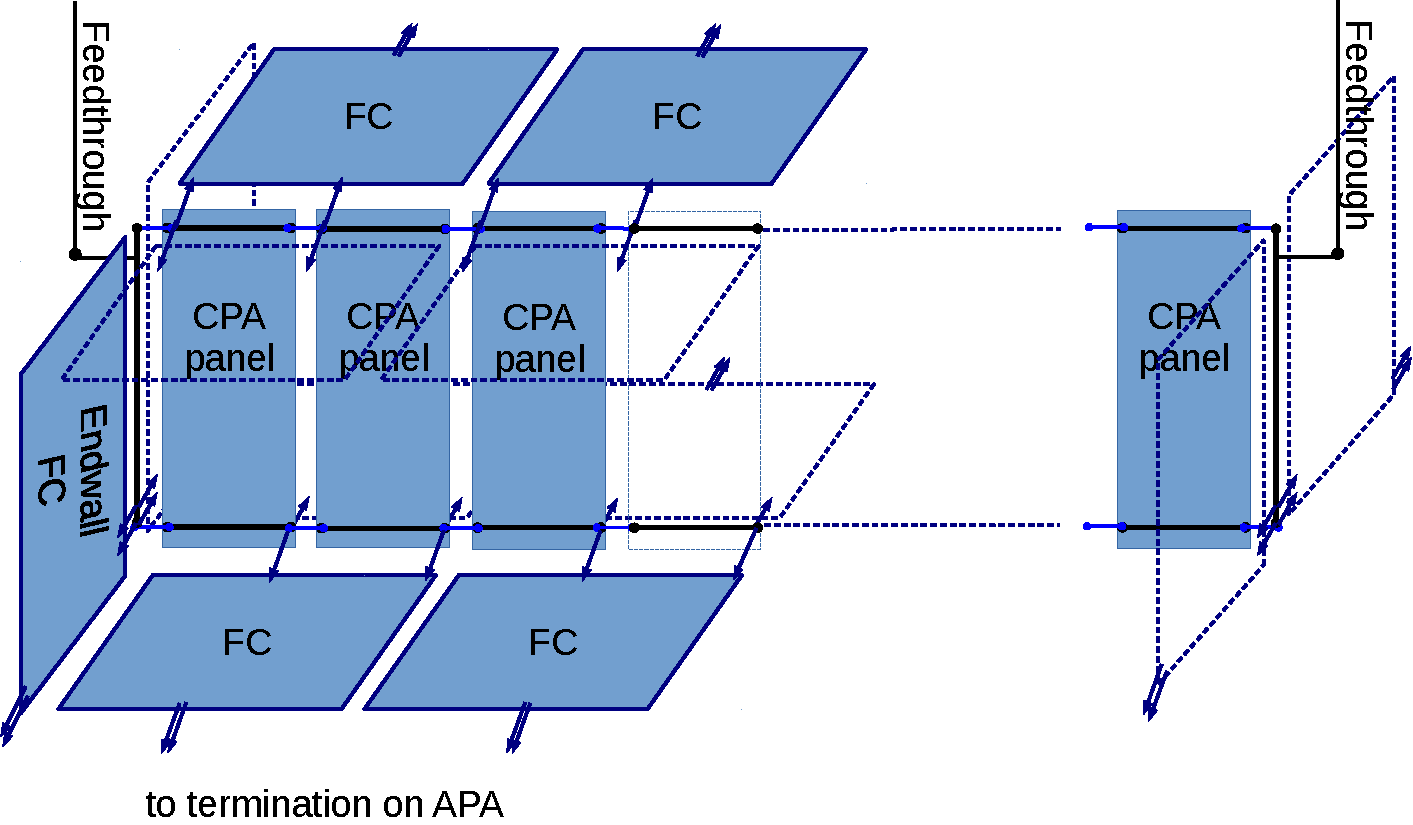
\includegraphics[width=0.7\textwidth]{fdsp-hv-interconnection-topology}
\end{dunefigure}

High voltage feedthroughs connect to cups mounted on the \dword{cpa} frame
%\cite the \dword{hv} delivery section
that attach to an \dword{hv} bus running through the \dword{cpa}s.  \Dword{hv} bus connections
between \dword{cpa} panels are made by flexible wires through holes in the
\dword{cpa} frame. The \dword{hv} bus is a loop that mitigates any risk of a single
failure point; the feedthrough at each end of each \dword{cpa} panel mitigate
risk of a double-break failure.  Voltage dividers on each \dword{cpa} panel
bias the \dword{fss} and the resistive dividers on the top
and bottom \dwords{fc}.  The \dword{cpa}-to-\dword{fc} connections are made using
flexible wire to accommodate \dword{fc} deployment.  To further
increase redundancy, two \dword{cpa} panels connect to each top or bottom
field cage, and two connections are also made to each \dword{ewfc}. Resistor divider boards attach directly to the interior side of
the \dword{fc} profiles with screws.   A redundant pair of flexible wires
connects a circuit board on the last profile of each \dword{fc} to a
bias-and-monitoring board mounted on the corresponding \dword{apa}.

%% connections within \dword{cpa}
Short sections of flexible wire at the ends of each \dword{hv} bus segment
attach to screws in brass tabs on the \dword{cpa} resistive panels (\dword{cpa} \dwords{rp}).
%\cite \dword{cpa} design subsection
Vertical \dword{hv} bus segments on the outer ends of each \dword{cpa} plane connect
the top and bottom \dword{hv} buses to complete the loop.  Solid wire is used
to connect resistive panels within a \dword{cpa} panel.

%% \dword{fc} connections
Each \dword{fc} module is as electrically independent as possible in order to
mitigate discharge.  However, only the bottom module of each endwall
can make connections to the \dword{hv} bus and \dword{apa}, so each endwall module
is connected to its upper neighbor at its first and last profile
using metal strips.

%% added by BY
Each \dword{fc} divider chain connects to an \dword{fc} termination board in parallel to a grounded fail-safe circuit at the \dword{apa} end.  The \dword{fc} termination boards are mounted on the top of the upper \dword{apa}s and bottom of lower \dword{apa}s.  Each board provides a default termination resistance, and an SHV cable connection to the outside of the cryostat, via the \dword{ce} signal feedthrough flange, through which we can either supply a different termination voltage to the \dword{fc} or monitor the current flowing through the divider chain.

%% Regarding wire terminals and screws
All flexible wires have ring or spade terminals and are secured by
screws in brass tabs.  Spring washers are used with every electrical
screw connection in order to maintain good electrical contact with
motion and changes of temperature.

Table \ref{tab:sp-hv-interconnects} summarizes the interconnections required 
for the \dword{hv} system.

\begin{dunetable}
[HV system interconnections]
{p{0.35\linewidth}p{0.62\linewidth}}
{tab:sp-hv-interconnects}
{\dword{hv} system interconnections}   
 Connection & Method \\ \toprowrule
 \dword{hv} cup to \dword{hv} bus & wire to screw in \dword{hv} cup mount on \dword{cpa} frame \\ \colhline
 \dword{hv} bus between \dword{cpa} panels & wire between screws in brass tabs \\ \colhline
 \dword{hv} bus to \dword{fss} & wire to circuit board mounted on \dword{fss} \\ \colhline
 \dword{fss} to \dword{topfc} and \dword{botfc} & wire to circuit board on first \dword{fc} profile, two per \dword{fc} module \\ \colhline
 \dword{hv} bus to endwall \dword{fc} & wire to circuit board mounted on first \dword{fc} profile, two per endwall \\ \colhline
 \dword{fc} divider circuit boards & directly attached to profiles using screws and SS slip nuts \\ \colhline
 \dword{fc} to bias and monitoring termination & redundant wires from board mounted on last \dword{fc} profile \\ \colhline
 \dword{hv} bus to \dword{cpa} panels & brass tab on \dword{cpa} resistive panel \\ \colhline
 \dword{cpa} \dword{rp} interconnections & solid wire between screws in brass tabs \\ \colhline
 Endwall \dword{fc} module interconnections & metal strips, first and last profiles only
 \\ 
\end{dunetable}

The redundancy in electrical connections described above meets requirement~\ref{ spec:hv-connection-redundancy }. %TOP Level requirement 6? 2? 5? SP-FD, SP-HV?
The \dword{hv} bus and interconnections are all made in low field regions in order to meet requirement \ref{ spec:local-e-fields }  %SP-FD-24.
The \dword{hv} bus cable is rated at the full cathode \dword{hv} such that even in case of a rapid discharge of the \dword{hv} system no current can flow to the cathode or \dword{fc} except at the intended contact points, preserving the ability of the resistive cathode and \dwords{fc} to meet requirement \ref{ spec:cathode-resistivity }. %SP-FD-17.

%%%%%%%%%%%%%%%%%%%%%%%%%%%%%%%%%%%%%%%%%%%%%%%%%%%%%%%%%%%%%%%%%%%%
\section{ProtoDUNE-SP High Voltage Experience}
\label{sec:fdsp-hv-protodune}



\dword{pdsp} \cite{Abi:2017aow} is a prototype for an \dword{spmod}. 
Approximately one twentieth the size of a \dword{spmod}, this detector implements an A-C-A configuration with one \dword{cpa} array that bisects the \dword{tpc} and two \dword{apa} arrays, one along each side. 
The \dword{cpa} array consists of %three full-size \dword{cpa} planes with dimensions \SI{2.3}{m} $\times$ \SI{6.0}{m} 
six \dword{cpa} panels, each \SI{1.2}{m} wide by \SI{6.0}{m} high (half-height relative to an \dword{spmod}), 
and is positioned \SI{359}{cm} away from each \dword{apa} array, matching the maximum drift distance of an \dword{spmod}.

Six top and six bottom \dword{fc} modules connect the horizontal edges of the \dword{cpa} and \dword{apa} arrays, and four %endwalls 
\dwords{ewfc} connect the vertical edges (two per drift volume). One of the drift volumes is pictured in Figure~\ref{fig:protodune_sp_hv}. 
Each \dword{ewfc} comprises four endwall modules (half-height relative to a \dword{spmod}).
A Heinzinger $-$\SI{300}{kV} \SI{0.5}{mA} \dword{hv} power supply delivers voltage to the cathode.
Two \dword{hv} filters in series between the power supply and \dword{hv} feedthrough filter out high-frequency fluctuations upstream of the cathode.

\begin{dunefigure}[Photo of ProtoDUNE-SP drift volume with HV components]
{fig:protodune_sp_hv}
{One of the two drift volumes of \dword{pdsp}. The \dword{fc} modules shown enclose the drift volume between the \dword{cpa} array (at the center of the image) and the \dword{apa} array (upper right). The \dwords{ewfc} are oriented vertically; the top and bottom units are horizontal. The staggered printed circuit boards connecting the \dword{ewfc} profiles are the voltage divider boards. %which introduce a uniform resistance between neighboring electrodes. (this part is in regular text Anne)
}
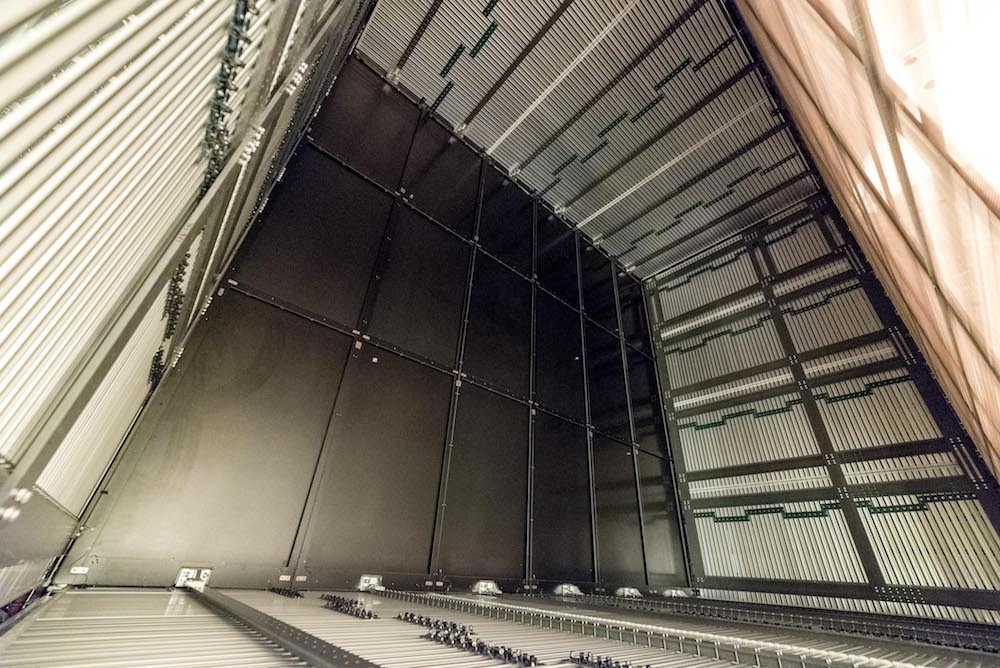
\includegraphics[width=0.8\textwidth]{protoDUNE-SP_TPCHV}
\end{dunefigure}

%%%%%%%%%%%%%%%%%%%%%%%%%%%%%%%%%%%%
\subsection{Summary of HV Construction}
\label{sec:fdsp-hv-protodune-summary}

The \dword{pdsp} \dword{hv} components underwent %some level 
various levels of pre-assembly offsite prior to transport and final assembly in the \dword{pdsp} cleanroom adjacent to the cryostat.

Parts for the top and bottom \dword{fc} frames were procured and test fit at Stony Brook University before being shipped to \dword{cern} for module assembly in a cleanroom about \SI{5}{km} away from the detector hall.
Fully assembled modules were transported individually to the detector hall for storage until installation. \dword{cern} provided the \dwords{gp} for the top and bottom \dwords{fc} as well as the field shaping profiles for all \dwords{fc}.


Louisiana State University (LSU) provided all the voltage divider boards, then procured and test fit the \dword{ewfc} frame parts before shipping them fully assembled to \dword{cern}.
These profiles and the voltage divider boards were installed in the same \dword{cern} cleanroom facility as the other \dword{fc} components.

Argonne National Laboratory shipped the \dword{cpa} material to the detector hall as single pre-assembled resistive panels held in a \frfour frame; i.e., as \dword{cpa} units (Table~\ref{tab:cpaparts}). 
In the cleanroom adjacent to the \dword{pdsp} cryostat, three \dword{cpa} units were mechanically and electrically connected to produce a \dword{cpa} panel. 
The \dword{cpa} panels (one of which is pictured in Figure~\ref{fig:cpa_panel-complete}) were first assembled horizontally and then lifted and rotated to a vertical orientation where they were paired to make a \SI{6.0 x 2.3}{m} \dword{cpa} plane.

At this point, two top and two bottom \dword{fc} modules were brought to the cleanroom to be lifted, rotated to vertical, and attached to the \dword{cpa} plane. 
To fit through the \dword{tco}, the top \dwords{fc} were suspended from their support at the top of the \dword{cpa} plane to hang vertically, and the bottom \dwords{fc} were folded up and temporarily attached to their top \dword{fc} counterparts.
The resulting \dword{cpa}-\dword{fc} assemblies were rolled onto the central bridge beam inside the cryostat and %subsequently 
deployed. 

Also in the \dword{pdsp} cleanroom, sets of four pre-assembled \dwords{ewfc} %panels 
were each assembled into one \dword{ewfc} plane. %s (four endwalls/plane). %end wall).
Although not a component of the \dword{spmod} design, 
the beam plug was installed onto its corresponding module %here 
before the beam-right, upstream \dword{ewfc} was built.
An electric hoist lifted the top %panel 
module to a height at which the next %panel 
module could be wheeled underneath and connected via \dword{frp} plates.
The hoist then raised the pair, and the procedure would continue in this way until the \dword{ewfc} was four %panels 
modules tall.
The load of the assembled endwall was then transferred to a trolley on a transport beam, which allowed it to be pushed into the cryostat onto the appropriate bridge beam.

The \dword{tpc} components of \dword{pdsp} were installed first for the drift space to the right of the delivered beam (beam-right), and then for the beam-left drift space.
The \dword{apa}s and the \dword{cpa} array were locked into position along their respective bridge beams, and then the bridge beams were locked into their positions along the drift direction.
Next, the two \dwords{ewfc} were moved and rotated into their upstream and downstream positions to bridge the gap between the vertical edges of the corresponding \dword{apa} and \dword{cpa}.
The \dwords{ewfc} loads were transferred onto the \dword{apa} and \dword{cpa}  bridge beams, which freed the intermediate bridge beam for top and bottom \dword{fc} deployment.
Two mechanical hoists were used to lower (raise) the bottom (top) \dword{fc} to bridge the gap between the horizontal edges of the \dword{apa}s and \dword{cpa}s.
Finally, the \dword{hv} cup was connected on the downstream \dword{cpa}, and the \dword{hv} feedthrough was lowered through the cryostat penetration to make contact with the cup.

%\subsection{HV Commissioning and Operation}
\subsection{HV Commissioning and Beam Time Operation}
\label{sec:fdsp-hv-commissioning-operation}
During \cooldown and \dword{lar} filling, a power supply was used to supply $-$\SI{1}{kV} to the cathode and monitor the current draw of the system.
As the system cooled from room temperature to \dword{lar} temperature, the resistance increased by $\sim$10\%, consistent with expectations.
Once the \dword{lar} level had exceeded the height of the top \dwords{gp}, the voltage was ramped up to the nominal voltage.



The initial week of \dword{hv} operations showed no signs of any anomalous instabilities. Over the following weeks, the \dword{hv} power supply showed signs of instabilities that affected the quality of the \dword{hv} provided to the cathode plane. Replacement of the power supply  midway through the run resulted in higher stability of the warm side of the \dword{hv} system. The original power supply was sent to Heinzinger for inspection. The malfunctioning was confirmed to be due to unexpected excessive moisture that had accumulated in the \dword{hv} cable socket.

In addition, % to the high voltage power supply issue, 
two types of instabilities emerged in the cold side of the \dword{hv} system. The first type was the so-called current blips, during which the system draws a small excessive current that persists for no more than a few seconds. The magnitude of the excess current during such events increased over the subsequent three weeks from 1\% to 20\%. The second type of instability, labeled ``current streamers,'' %during which there was 
exhibited persistent excessive current draw from the \dword{hv} power supply with accompanying excessive current detected on a \dword{gp} and on the beam plug. These two types of instabilities were experienced periodically throughout the duration of the \dword{pdsp} beam run. The frequency of both types increased over time after the system was powered on, until a steady state of about ten current blips/day and one current streamer  every four hours was reached. These effects are consistent with a slow charging-up process of the insulating components of the \dwords{fc} supports, which then experience partial discharges that are recorded as \dword{hv} instabilities. This process appears to restart after every long \dword{hv}-off period. 

In addition, these processes seem to be enhanced by the \dword{lar} bulk high purity, which allows the electric current to develop. 
At low purity electronegative impurities act as quenchers, blocking the development of the leakage current. Despite the presence of two types of instabilities, the \dword{hv} system was able to consistently achieve >95\% uptime during the beam runs. The downtime was the result of short manual interventions to quench a current streamer (Figure \ref{fig:protoDUNE-SP_beamRunSum_HV}).

In some cases, %mainly when there was no beam run ongoing, 
mostly outside of the beam run period, we turned off the \dword{hv} system momentarily to allow the \dword{hv} system components to discharge. This is reflected as larger dips in the uptime plot. During moments when the rest of the subsystems (including the beam) were stable, the moving 12-hour \dword{hv} uptime fluctuated between 96\% and 98\%.



\begin{dunefigure}[ProtoDUNE-SP HV performance during the test beam run]
{fig:protoDUNE-SP_beamRunSum_HV}
{The performance of the \dword{hv} system across the test beam period, September-November 2018. The top panel shows the drift field delivered to the \dword{tpc}, the middle panel indicates \dword{hv} cuts during periods when the system is not nominal (some periods not visible due to their short timescale), and the bottom panel shows the moving 12-hour uptime of the \dword{hv} system based on these \dword{hv} cuts.}
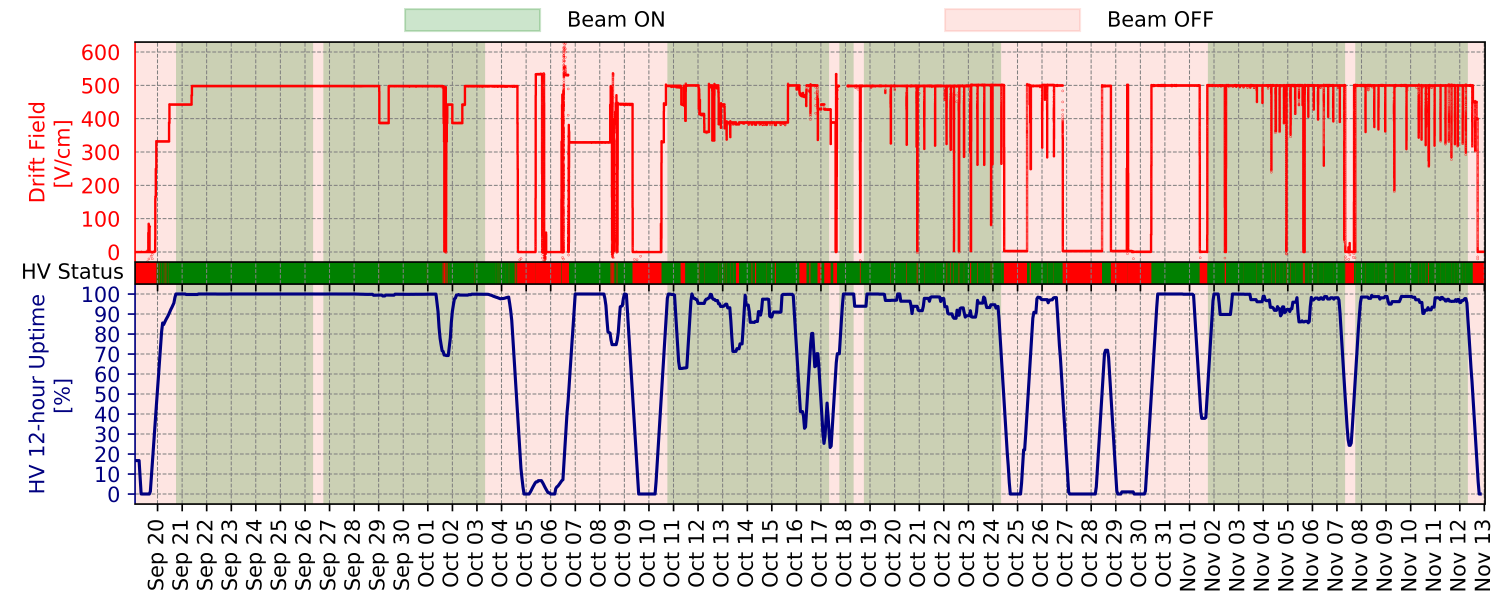
\includegraphics[width=\textwidth]{protoDUNE-SP_beamRunSum_HV}
\end{dunefigure}

The up-time during the week starting October 11th (Oct 11 in Figure \ref{fig:protoDUNE-SP_beamRunSum_HV}) is lower than the subsequent three beam-on weeks because the current streamers were addressed differently in these two periods. In the beginning, they were left to develop until they quenched themselves or until the \dword{hv} was manually ramped down. The \dword{hv} was brought back up when the current draw returned to nominal, according to the \dword{fc} resistance value. Automated controls to quench the current streamers were then successfully implemented in an auto-recovery mode. These helped significantly to increase the up-time, by optimizing the ramping down and up of the \dword{hv} power supply voltage, which was performed in less than four minutes (Figure \ref{fig:HV_autorecovery}).

\begin{dunefigure}[ProtoDUNE-SP HV autorecovery procedure]
{fig:HV_autorecovery}
{Example of the \dword{hv} automatic recovery procedure developed to detect and quench the current streamers: whenever an excess sustained current from the \dword{hv} PS is detected (obtained by continuously monitoring the total detector resistance experienced by the PS), the \dword{hv} delivered by the PS is lowered in discrete steps. At each step the total resistance is checked again, and if it agrees with the nominal detector resistance the \dword{hv} is ramped up again to its nominal value; otherwise the \dword{hv} is lowered to the next step.}
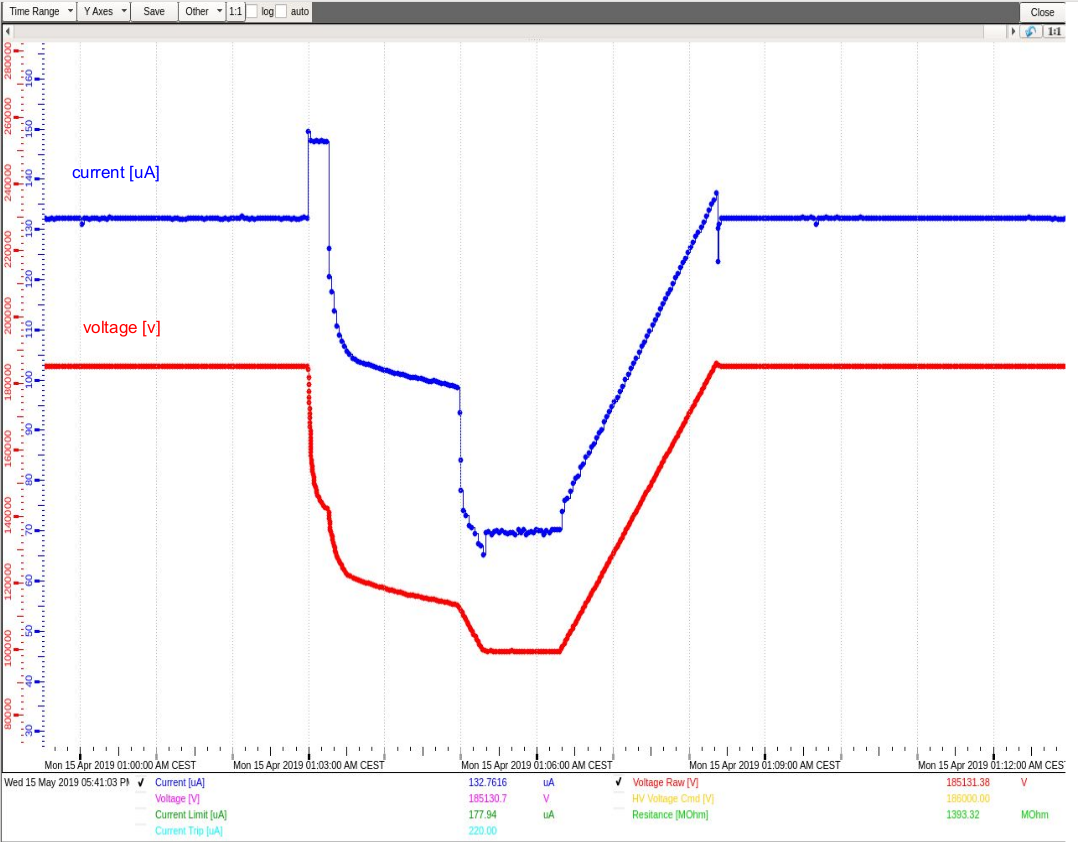
\includegraphics[width=0.5\textwidth]{HV_autorecovery}
\end{dunefigure}



\subsection{Post-beam Stability Runs with Cosmic Rays}
\label{sec:fdsp-hv-long-term-operation}

During the 2018 beam run periods, priority was given to operating the \dword{pdsp} detector with maximal up-time in order to collect as much beam data as possible at the nominal \dword{hv} conditions. Therefore, investigating the long-term behavior of the \dword{hv} instabilities and understanding their origin became goals of the long-term operation of \dword{pdsp} in 2019.

As mentioned above, it appears that the current streamer effect is a charging-up process with its frequency increasing with time after a long \dword{hv}-off period. This behavior has been repeatedly observed and confirmed in 2019. The current streamer rate stabilized at 4-6 per day, and the location was essentially always on the same single Ground Plane (GP\#6) out of the 12 monitored \dwords{gp}. Their rate and location were approximately independent of the \dword{hv} applied on the CPA in the $\SI{90}{kV}$ to $\SI{180}{kV}$ range.

More recently, after a change of the \dword{lar} re-circulation pump (April 2019), the detector was operated for several months in very stable cryogenic conditions and with very high and stable \dword{lar} purity (as measured by purity monitors and cosmic rays). During this period, the \dword{hv} system was set and operated at the nominal value of 180 kV at the \dword{cpa}  for several weeks without interruption. A significant evolution in the behavior of the \dword{hv} system was observed. 

To better understand the current streamers phenomenon, the \dword{hv} system was operated for about fifty days without the auto-recovery script, and the current streamers were left to evolve naturally. They typically lasted 6 to 12 hours, exhibiting steady current and voltage drawn from the \dword{hv} power supply and they eventually self-quenched without any intervention. The repetition rate was highly reduced to about one current streamer every 10-14 days; this rate can be compared to the 4-6 per day in the previous periods with auto-recovery on.

The auto-recovery script was then re-enabled and the current streamer rate stabilized at about one in every 20 hours; in addition, the intensity of the current streamer on the \dword{gp} was reduced with respect to the previous periods. As in the previous runs, the current streamers occurred always on the same \dword{gp} (GP\#6) with a small leakage current on the beam plug hose, which is close to GP\#6. 

This behavior is a further indication that the current streamers are in fact a slow discharge process of charged-up insulating materials present in the high-field region outside of the \dword{fc}. The auto-recovery mode does not allow a full discharge, so the charging up is faster, and the streamer repetition rate is shorter.

The \dword{lar} purity loss experienced at the end of July, 2019, was accompanied by the complete disappearance of any \dword{hv} instabilities. 
They gradually reappeared when the electron lifetime again exceeded 200 microseconds, and their intensity constantly increased as purity improved. This behavior replicated that observed after the initial filling, and supports the hypothesis that the \dword{hv} instabilities are enhanced by the absence of electronegative impurities in high-purity \dword{lar}.

The effects of the current streamers on the \dword{fe} electronic noise and the \dword{pd} background rate have been investigated. We have not observed any effect of the current streamers on the \dword{fe} electronics. On the other hand, recent analysis of the data collected by the \dword{pds} during active current streamers has indicated a high single photon rate on the upper upstream part of the \dword{tpc}. This is consistent with the activities recorded on GP\#6, which is located exactly at this upper upstream area. The analysis of the photon detection data is in progress with the main goal of narrowing down the position of current streamers and the localization of it, if possible (Figure~\ref{fig:PD_activity_on_streamers})
Visual inspection of this location when the detector is emptied will be required to further understand the \dword{hv} instability issues.

\begin{dunefigure}[Photon detector activity on streamers]
{fig:PD_activity_on_streamers}
{Preliminary analysis of the single photon activity rate in coincidence with a current streamer as a function of the position of the \dwords{pd} in the \dword{apa}s (beam right site). The rate clearly decreases proportionally to the distance of the \dword{pd} from the supposed location of the current streamer. More refined analysis is ongoing (including the beam left \dwords{pd}) to better locate the light source.}
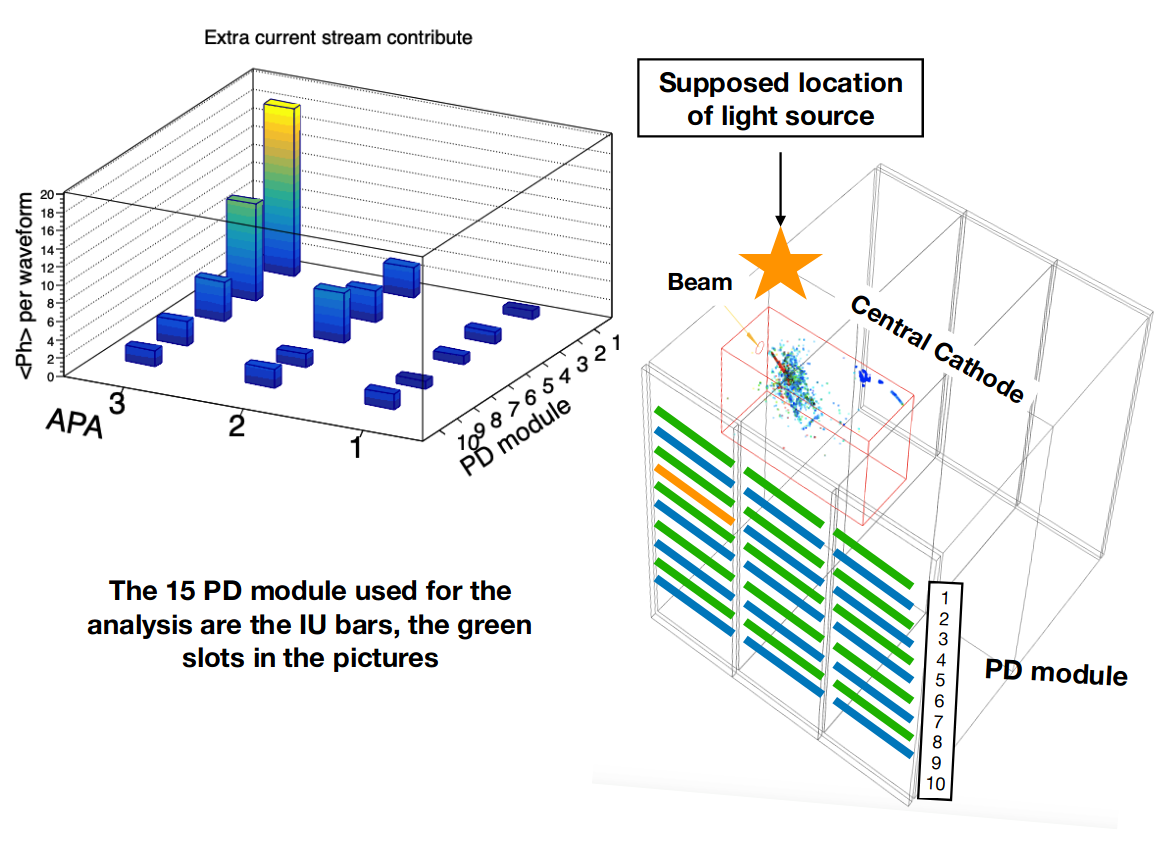
\includegraphics[width=0.75\textwidth]{PD_activity_on_streamers}
\end{dunefigure}

It is planned to continue monitoring the \dword{hv} behavior, and in particular, before the end of the run, we plan to increase the \dword{hv} above the nominal value to possibly enhance anomalous effects in the \dword{hv} chain. Furthermore, the possible role of macroscopic impurities (metallic or insulating dust) circulation within the \dword{lar} is still to be understood, and specific running conditions will be implemented in \dword{pdsp} to better investigate this issue as well. 

Although %at the moment, 
we do not yet have %fully 
precise knowledge of the origin of the current streamers, it is certainly safe to state that, in a time scale of nearly one year, we did not observe any degradation of the \dword{hv} system performance. On the contrary, the up-time has constantly improved (now it is above 99\%), and the instability rate and intensity have decreased. 

%%%%%%%%%%%%%%%%%%%%%%%%%%%%
\subsection{Lessons from ProtoDUNE}
\label{sec:fdsp-hv-protodune-lessons}

The \dword{pdsp} \dword{hv} experience was, in general, very encouraging, having demonstrated 
an ability to operate the \dword{tpc} with a drift field of \spmaxfield{}. % was demonstrated.
However, throughout the run, the system experienced various instabilities, %the understanding of which has %in the process of being investigated further been 
discussed above. 
Systematic study of these instabilities continues.

%%%%%%%%%%%%%%%
\subsubsection{Design}
\label{sec:fdsp-hv-protodune-lessons-design}

The success of \dword{pdsp} validated the general design of the DUNE \dword{hv} system, but various opportunities for improvement during its construction and operation appeared. %were found.
 In particular, we chose the following:

\begin{itemize}
\item adopt a ``pot-style'' filter resistor design (with input and output cables on the same end) %would 
to prevent leaks from causing interventions for refilling;
\item raise the \dword{hv} feedthrough cable insert to be above the cold insulation space, if space allows (to allow removing the cable while preventing moisture from entering and freezing on the walls, which could affect electrical contact);
\item add toroid signals %would be a welcomed addition 
to the feedthrough; and
\item improve stability by increasing the distance between the \dwords{gp} and field-shaping profiles and eliminating direct paths for potential surface currents.
\end{itemize}


The instrumented \dwords{gp} on the top and bottom \dwords{fc} proved invaluable for collecting information during moments of instability.
A dedicated \dword{daq} read out the signals from the \dword{gp} monitoring system, the beam plug current monitor, and the power supply at a rate of \SI{20}{kHz} on a trigger provided useful information for diagnosing the \dword{hv} behavior inside the \dword{tpc}.
This system was not operated continuously due to correspondingly large data disk storage requirements.
Toroid signals from the \dword{hv} filters were also helpful in localizing sources of instability, specifically for distinguishing issues on the warm side from issues inside the \dword{tpc}.


  %edit by demuth



%%%%%%%%%%%%%%%
\subsubsection{Production, Handling and Quality Control}
\label{sec:fdsp-hv-protodune-lessons-prod}

The production and handling of \dword{hv} components must be approached with %sufficient 
great care to avoid scratching and potentially compromising the electrical components. 
Part production should be carried out to avoid introducing sharp edges wherever possible.
The corners of the \dword{gp} panels had to be smoothed after some buckling was introduced during the pressing process, and a number of support hinges and clevises had sharp features removed by polishing.
The aluminum field-shaping profiles are particularly prone to scratches and must be packaged and handled so as to avoid direct contact with other profiles and materials.
Kapton strips were used to separate the profiles from the \dword{frp} of the \dword{fc} frames as they were being inserted to protect against scratching or removal of the profile coating.
Any scratches found in the \dword{frp} beams were covered with epoxy to prevent fibers from escaping into the \dword{lar}.

\Dword{qc} tests were conducted on \dword{hv} modules and individual components at every step: %of the construction:  
part procurement, production, integration, and installation.  For example, checklist forms were completed for component parts of detector modules as production proceeded.  Also, during the production process, documented procedures included \dword{qc} steps with checklist forms.  Printed copies of the checklists completed in the procurement and production stages were included as travelers in shipping crates.  
To ensure that nothing was compromised during transport, \dword{qc} tests were repeated on individual components and assembled pieces after shipping. 
Resistance between steps on the voltage divider boards was measured and verified to be within specification both after their production at LSU and after they were shipped to \dword{cern}.
Once the voltage divider boards were mounted onto an assembled \dword{fc} module, the resistance between adjacent profiles was measured to verify sound electrical connection.
In a similar way, \dword{qc} checks of connections between \dword{cpa} modules and between \dword{cpa} and \dword{fc} modules were performed after installation.

\dword{qc} tests on the \dword{hv} components of \dword{pdsp} required many measurements to be made with several different test devices.  Extrapolating these measurements to the scale of DUNE will require development of dedicated tools so that the \dword{qc} process can be made more efficient and optimal at each step.
%It was a tedious process to measure each voltage step individually several times each.
For example, devices to measure the resistivity of \dword{cpa} coated resistive panels and field shaping strips will be provided to each of the designated production factories.  Also, designing a rig that can latch onto the \dword{fc} modules in such a way to make contact with all electrodes and control their voltages independently would allow for an automated loop across all steps.
Such dedicated equipment and automated procedures will be required en route to a full \dword{spmod}.

%%%%%%%%%%%%%%%
\subsubsection{Assembly and Installation}
\label{sec:fdsp-hv-protodune-lessons-assy}

The \dword{pdsp} experience allowed for a realistic estimation of the time involved to produce various \dword{hv} components for an \dword{spmod}.
The time involved for \dword{pdsp} was approximately as follows:
\begin{itemize}
\item \dword{fc} module assembly: 1.5 days/module with 2 workers,
\item \dword{ewfc} module assembly: 1.5 days/module with 2 workers, 
\item \dword{cpa} (2-panel) plane: 2 days/plane with 4 workers,
\item \dword{cpa} plane + \dword{fc} integration: 1 day/assembly with 4 workers,
\item \dword{ewfc} frame assembly: 7 days/module with 2 workers,
\item \dword{ewfc} final assembly: 4 hours/wall with 4-6 workers.
\end{itemize}
These estimates include time needed to perform the required \dword{qc} tests at each stage of the assembly and installation.

%During installation, there were some concerns about various alignment issues with the \dword{tpc}, but essentially all issues were corrected once the entire detector was in place.
The \dword{pdsp} installation sequence had the beam-right drift volume deployed before the beam-left.
As anticipated from calculation and testing, asymmetries in the weight distribution before the beam-left drift was deployed produced temporary misalignments that propagated throughout the entire detector until the final left drift deployment, which corrected them.
The process of connecting individual endwall modules to build an endwall exposed another alignment issue.
The first endwall was %turned out 
significantly bowed initially.
A tool was built to adjust the angle between adjacent modules, which straightened out the wall.
The tool was also used while connecting modules for the remaining three endwalls, and no significant bowing was observed.


%%%%%%%%%%%%%%%%%%%%%%%%%%%%
\subsection{Future R\&D}
\label{sec:fdsp-hv-protodune-RD}

The present \dword{hv} system design derives closely from the one in operation in \dword{pdsp}.  Operation of this detector in 2019 has allowed us to gain further confidence in depth concerning the long term stability and reliability of the \dword{hv} system under nominal conditions.  The present R\&D program, which will not extend beyond early 2020, has the goal to further improve, if required, the reliability of the system.   
In the R\&D program we plan to  

\begin{itemize}
\item evaluate the charge and discharge behavior of the \dword{uhmwpe} caps on the end of the profiles compared to metallic capped profiles.  The goal is to check if the end caps contribute to \dword{hv} instability. 

\item compare the high voltage stability of a new version of end wall profiles to the \dword{protodune} version.  The new version bends the top and bottom of the end wall profiles 90 degrees towards the ends of the top or bottom profiles, reducing the gap between field cage components at the two detector module ends and lowering the \efield{}s on the surfaces of the \dword{uhmwpe} caps and profiles near the profile ends.
\item evaluate resistive versus metallic caps.  If the \dword{uhmwpe} caps are %shown to be 
problematic, find an alternative solution to maintain separated \dword{fc} modules.
\item study the surface-charging behavior of the \dword{fc} insulation structures.  Evaluation of general insulator performance for \dwords{lartpc}, including charge-up effects and geometry, remains an outstanding task.  In this test, the goal is to find out if any geometrical feature or surface treatment can reduce \dword{hv} instability.
\item evaluate higher-resistivity Kapton films.  The goal is to check the feasibility of increasing the surface resistivity of the cathode plane up to 1~G$\Omega$/square.  The task includes verifying the lamination quality on \frfour sheet and production availability.
\item perform further simulation of  \dword{hvs} discharge behavior. Although modeling other \dword{fc} designs and DUNE itself will take considerable effort, % the possibility of 
understanding the source of instabilities or exposing any design weaknesses would be worthwhile. %makes this a worthwhile endeavor.
\end{itemize}

%%%%%%%%%%%%%%%%%%%%%%%%%%%%%%%%%%%%%%%%%%%%%%%%%%%%%%%%%%%%%%%%%%%%
\section{Interfaces }
\label{sec:fdsp-hv-intfc}


The \dword{hvs} has the largest surface area on the \dword{tpc} and interfaces with many other systems.  Table~\ref{tab:HVinterfaces} summarizes the interfaces with other consortia, highlights the key elements, and provides the links to the existing interface documents.

The two most important mechanical interfaces are with the \dword{dss} and the \dword{apa}.  The entire weight of the \dword{cpa}s, \dword{ewfc} and half the weight of the top and bottom \dword{fc} are supported by rails provided by the \dword{dss}.  The other half of the top and bottom \dword{fc} weight is transferred to the \dword{apa}s through latches mounted on the \dword{apa}s. All \dword{cpa}s and most of the \dword{fc} modules are also transported along the DSS rails to their final positions. The \dword{dss} rails ultimately determine the final locations of the \dword{cpa}s and \dwords{fc} on the \dword{tpc}.

Electrically, since the \dword{apa}s are at the detector ground, all \dword{hvs} field cage termination and fail-safe circuits are connected to the \dword{apa}s.  All cables used for the \dword{fc} termination pass through the \dword{apa} frame, to connect to the \dword{shv} cables provided by the \dword{ce} through the \dword{ce} signal flanges.  The \dword{tpc} electronics consortium also provides \dword{hvs} the \dword{fc} termination power supplies.

\begin{dunetable}
[HV system interfaces]
{p{0.25\textwidth}p{0.5\textwidth}l}
{tab:HVinterfaces}
{\dword{hv} system interface links }   
Interfacing System & Description & Linked Reference \\ \toprowrule
\dword{dss}  &  Support, positioning, and alignment of all \dword{cpa}, \dword{fc} modules inside the cryostat both warm and cold & \citedocdb{16766}  
\\ \colhline
\dword{apa} & \dword{fc} support (top, bottom, and end wall) on \dword{apa} frames; Mounting of FC termination filter boards and \dword{fc} fail-safe terminations; 
%% EDs are APA's responsibility (BY)
%% Mounting of the electron diverter boards.
& \citedocdb{6673} 
\\ \colhline
\dword{ce} & \dword{fc} termination wire connectors on CE feedthrough flange, \dword{fc} termination wires routed with CE cables & \citedocdb{6739} 
 \\ \colhline
\dword{pds} & Mounting of PD calibration flash diffusers and routing of their fibers to \dword{cpa}s; Possible \dword{tpc} coated reflector foil on \dword{cpa}s. & \citedocdb{6721} 
 \\ \colhline
facility & Locations and specifications of the \dword{hv} \fdth ports; gas and \dword{lar} flow velocities and patterns. & \citedocdb{6985}  
\\ \colhline
calibration & \dword{fc} openings for the calibration laser heads & \citedocdb{7066}
\\ \colhline
\dword{cisc} & \dword{hv} vs. \dword{lar} level interlock, sensor locations in high field regions, cold/warm camera coverage, \dword{hv} signal monitoring, etc. & \citedocdb{6787} 
 \\ \colhline
%\dword{itf} No more ITF!
\dword{sdwf} & Storage buffer, inspections/tests, repackage for underground delivery & \citedocdb{7039} 
 \\ \colhline
physics & Requirements: range of operating drift field, uniformity of the drift field; Supply detector geometry and \efield{} map. & \citedocdb{7093} 
 \\ 
\end{dunetable}

%%%%%%%%%%%%%%%%%%%%%%%%%%%%%%%%%%%%%%%%%%%%%%%%%%%%%%%%%%%%%%%%%%%%
\section{Production and Assembly }
\label{sec:fdsp-hv-prod-assy}

%%%%%%%%%%%%%%%%%%%%%%%%%%%%
\subsection{Power Supplies and Feedthrough}
\label{sec:fdsp-hv-supplies-feedthrough}

We plan to buy commercial power supplies through, among other vendors, Heinzinger. 
The \dword{hv} cable is commercially available.

The power supply is tested extensively along with the controls and monitoring software.  Features to be included in the software are
\begin{itemize}
\item the ability to ramp, or change, the voltage, set the ramp rate, and pause the ramp. % The rate and an ability to pause the ramp shall be included.  
In previous installations, the ramp rate was typically between \SIrange{60}{120}{V/s}.
\item an input for a user-defined current limit.  This parameter is the electric current (I) value at which the supply reduces the voltage output to stay below the current limit.  The current-limiting is done in hardware.
\item an input for a trip threshold.  At this current reading, the program would reduce the voltage output through software.  In previous experiments, the trip function in software would set the output to \SI{0}{kV}.
\end{itemize}
Additionally, the software must
record the current and voltage read-back values with a user-defined frequency, as well as any irregular current or voltage events.



The \dword{hv} feedthrough and filters are custom devices. As for \dword{pdsp}, the feedthrough  designs are made by collaborators and fabricated by an external company or major laboratory.
 Raw materials such as stainless steel, \dword{uhmwpe} rods, and flanges are readily available and are machined to make a feedthrough. Similarly, the resistors, steel or aluminum, and insulator material for the filters are readily available. The feedthrough and filters require testing before being delivered to the \dword{sdwf}. %ITF.  
 
%%%%%%%%%%%%%%%%%%%%%%%%%%%%
\subsection{Cathode Plane Assembly}
\label{sec:fdsp-hv-prod-cpa}
 The component parts of the \dword{cpa} array will be mainly produced by commercial companies except for specific items that are more efficiently produced by university collaborators.  Parts will be packaged into kits, each to contain the parts for a single \dword{cpa} panel
(three \dword{cpa} units). The parts in each kit are

\begin{itemize}
\item manufactured \frfour \dword{rp} frames, % packed into kits for a single \dword{cpa} panel (three \dword{cpa} units),
\item carbon-impregnated Kapton-coated \dwords{rp} and \dword{fss},
\item \dword{hv} cable segments and wire jumpers making up the \dword{cpa} \dword{hv} bus and \dword{rp} interconnects,
\item resistor boards connecting the \dwords{rp} to \dword{fss} (for raising the \dword{rp} \dword{hv} by \SI{1.5}{\kV}),
\item machined brass tabs for connecting \dwords{rp}, \dword{hv} bus, and \dword{fss}, and
\item top, bottom, and exterior edge profiles and associated connection hardware.
\end{itemize}
The kits are sent to the production factories, the locations of which will be determined later.  
The %basic 
\dword{cpa} construction unit for installation into the \dword{spmod} at the \dword{surf} is a pair of \dword{cpa} panels called a \dword{cpa} plane. The production factories thus ship partially-assembled \dword{cpa} panels to \dword{surf} where panel assembly is completed and two panels are paired in the underground cleanroom to form a \dword{cpa} plane. During production, some storage (up to one month's installation rate) of \dword{cpa} shipping crates can occur at the \dword{sdwf} while waiting for movement into the \dword{surf} cleanroom.  No unpacking of crates is needed at the \dword{sdwf}; only visual inspection will be done to determine if any damage occurred during shipping.

The most basic element of the \dword{cpa} 
is an \dword{rp} mounted in a machined slot in the top, bottom and sides of \frfour frames.  
There are three different \dword{rp} types: an upper, which has as its top frame the \dword{cpa} mounting bracket and \dword{topfc} hinge, a middle, and a lower, which has as its bottom frame a \dword{botfc} hinge.  
Pairs of \dwords{rp} are bolted together and pinned to form \dword{cpa} units of size \SI{1.2}{\m} $\times$ \SI{4}{\m} for shipment. Three types of pairings are constructed to make a full six-\dword{rp}, \SI{12}{\m} tall \dword{cpa} panel: (1) an upper and a middle, (2) two middle, and (3) a middle and a lower.

The order in the shipping crate from top to bottom is: middle-and-lower, middle-and-middle, and upper-and-middle.   Two \dword{cpa} panels are shipped together in one crate; they are paired at \dword{surf} to form one \dword{cpa} plane.  The \dword{spmod} requires 100 upper, 100 lower, and 400 middle \dwords{rp} to make up the 100 \dword{cpa} panels (50 \dword{cpa} planes) of the \dword{tpc}.


In addition to the frames and \dwords{rp}, 
\dword{fss} are mounted on the exposed sides of the \frfour frames, aluminum profiles are attached to the exterior edges of the upper and lower \dwords{rp}, 
and cables are attached to the \dwords{rp} to form segments of the \dword{hv} bus.  

The \dword{cpa} units are assembled horizontally on a smooth, flat, highly stable table 
to ensure flatness and straightness of the entire panel before units are pinned together. There is one table per factory with up to three factories making \dword{cpa}s.

Figure~\ref{fig:12m-cpa} shows a  \SI{6}{\m} \dword{pdsp} \dword{cpa} panel (rear) and a \SI{12}{\m} \dword{pdsp} \dword{cpa} panel (foreground) at \dword{ashriver} Laboratory in Minnesota, USA.


\begin{dunefigure}[CPA mockup panels at Ash River]{fig:12m-cpa}{A \SI{12}{\m} DUNE-SP \dword{cpa} mock-up panel (foreground) and a %smaller 
half-height \SI{6}{\m} \dword{pdsp} panel mock-up (rear) at \dword{ashriver}, Minnesota.}  %closest panel 6m, each strip separated by 2m, this image taken in the pit at Ash River (where NOvA modules were stacked/glued.)
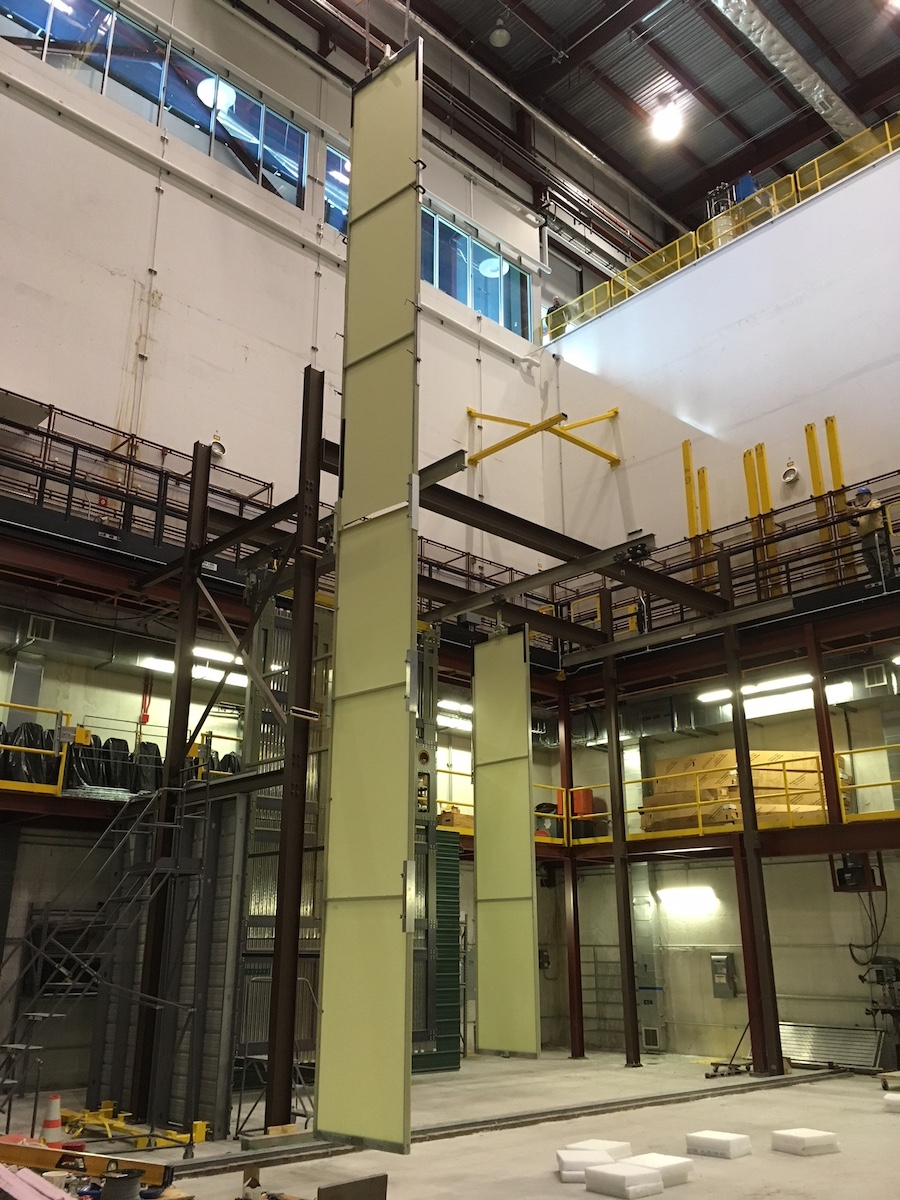
\includegraphics[width=0.5\textwidth]{12m-cpa}
\end{dunefigure}

%%%%%%%%%%%%%%%%%%%%%%%%%%%%
\subsection{Field Cages}
\label{sec:fdsp-hv-prod-fc}



\subsubsection{Top and Bottom Field Cages}
\label{sec:fdsp-hv-prod-fc-tb}

Firms that specialize in the machining of fiberglass components for electrical applications will produce the \dword{frp} and \frfour components of the top and \dwords{botfc}, as was successfully done for \dword{pdsp}. 
All the machined edges except the small circular holes are to be coated with translucent epoxy. The stainless steel and aluminum components will be produced in university and commercial machine shops. University groups will likely fabricate the voltage divider boards and \dword{fc} and \dword{cpa} connection boards.

The \dword{frp} frame assembly process consists primarily of fastening together \dword{frp} I-beams with \dword{frp} threaded rods and hex nuts,  and securing them with a limited and specified torque to avoid damage to the threads. Detailed views of this procecure %one of these connections 
are shown in Figure~\ref{fig:tbfc3}.

\begin{dunefigure}[Top and bottom FC module frame assembly procedure]{fig:tbfc3}{The figure shows the procedure for connecting the cross beams to the main I-beams for the \dword{topfc}. Left: A display of the components of each connection, which (from top to bottom) are the threaded rods, the spacer tubes, washer plates, the hexagonal nuts, and an L-shaped \dword{frp} brace. An intermediate stage (middle) and final stage (right) of the assembly are also shown.}
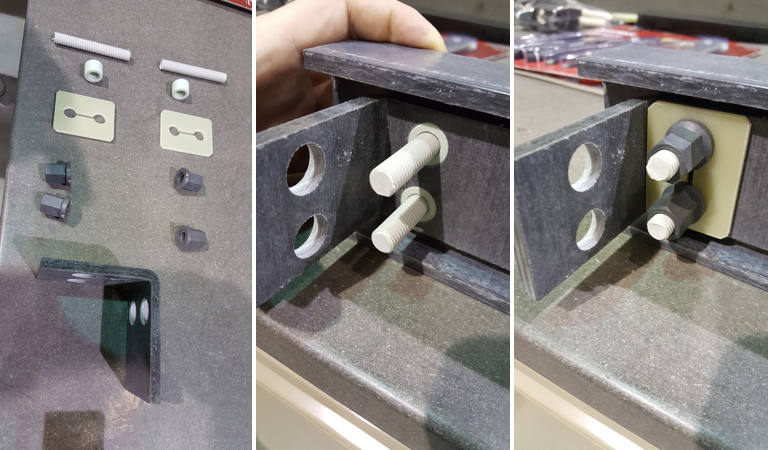
\includegraphics[width=0.70\textwidth]{tbfc3}
\end{dunefigure}

Prior to sliding each profile into the \dword{frp} frame, the holes %should be (should be? Anne changed to are)
are covered with Kapton tape to avoid damage to the profile coating. An end cap is attached to each profile using plastic rivets, and then the profiles are aligned against an alignment fixture running the length of the \dword{fc}. After securing each profile to the frame, the tension in the mounting screws is adjusted to remove any angular deflection in the extended portion of the profile.

The \dwords{gp} are attached to the \SI{10}{\cm} stand-off I-beam sections with threaded rods and a machined plate. The copper strips are connected to adjacent modules at the same locations. Care must be taken to avoid bending the corners of the \dwords{gp} toward the profiles, particularly on the \dword{cpa} side of the module.

%%%%%%%%%%%%
\subsubsection{Endwall Field Cages}
\label{sec:fdsp-hv-prod-fc-endw}

For the \dwords{ewfc}, all \dword{frp} plates are commercially cut to shape by water jet, as are the cutouts in the \dword{frp} box beams. % are also cut by water jet. 
Holes that accommodate G10 bushings are reamed in a machine shop. \dword{frp} frames are pre-assembled to ensure proper alignment of all \dword{frp} parts and %matching of 
holes (the profiles are not inserted at this stage). The \dword{frp} modules are hung off of each other by means of interconnecting \dword{frp} plates to ensure accurate alignment.

Next, parts are labeled, and the frames are taken apart. All components are cleaned by pressure washing or ultrasonic bath. All cut \dword{frp} surfaces are then coated with polyurethane, which contains the same main ingredient as the \dword{frp} resin, allowing it to bond well to the \dword{frp} fibers. Final panels are constructed from cleaned and inspected parts. Since assembly requires access to both sides of a module,
a dedicated assembly table has been manufactured that allows convenient module rotation. 

Figure~\ref{fig:endwall_assy_rot_table} shows a partially assembled \dword{ewfc} \dword{frp} frame on the assembly table.
\begin{dunefigure}[Endwall FC assembly table]{fig:endwall_assy_rot_table}{Assembly table with partially assembled \dword{ewfc} module. Box beams, cross beams, and slots for mounting of aluminum profiles are visible.}
 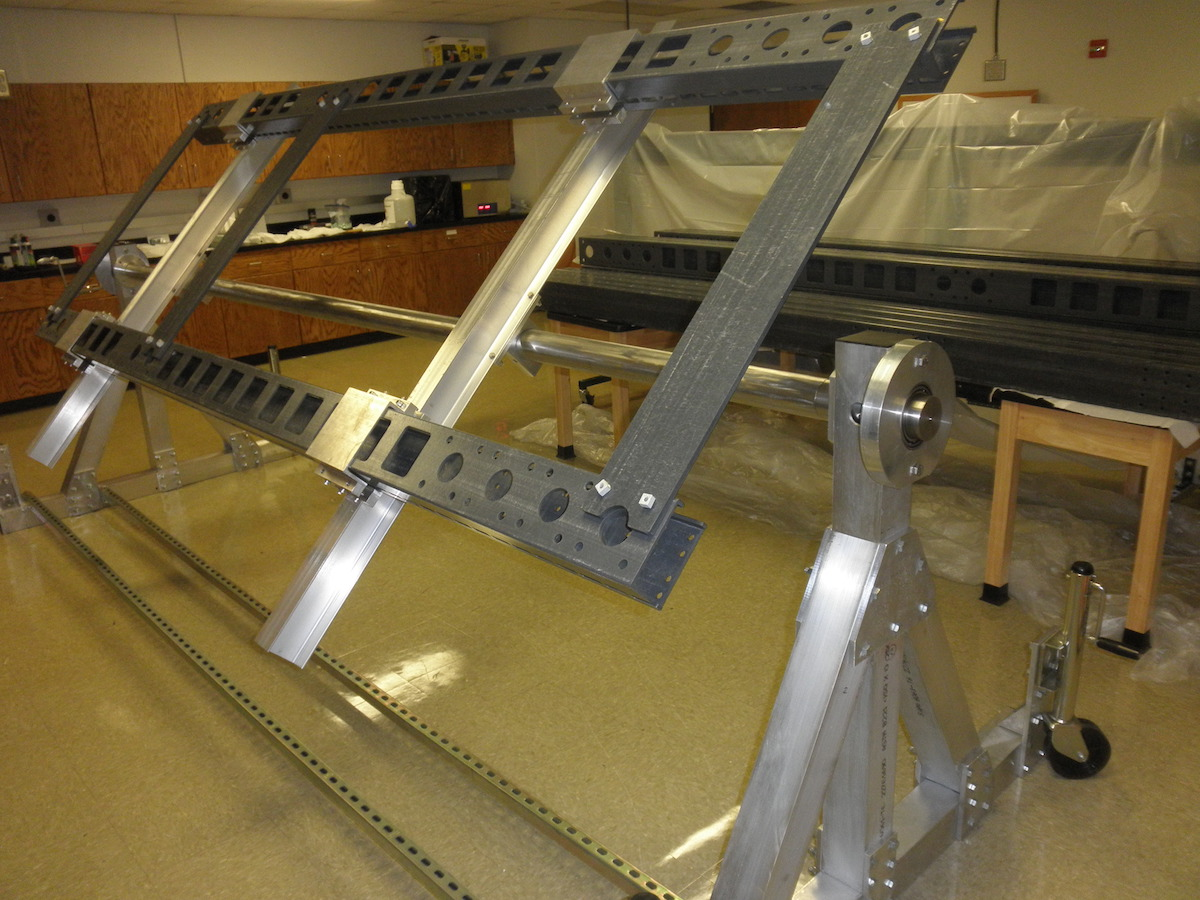
\includegraphics[width=0.8\textwidth]{endwall_assy_rot_table}
 \end{dunefigure}
The \dword{frp} box beams are sandwiched between \SI{1.27}{\cm} (\num{0.5}\,in) thick \dword{frp} panels that are held on one side by means of G10 bushings and rods with square nuts.
On the other side M10 stainless steel bolts, which are clearly visible in Figure~\ref{fig:endwall_assy_detail},  
engage with large slip nuts that are inserted into the aluminum profiles. The profiles 
are pulled towards a \SI{2.5}{\cm} thick \dword{frp} plate located 
on the inside of the box beam.
%

\begin{dunefigure}[Hanging endwall FC frames] %assembly 
{fig:endwall_assy_detail}{%Left: Side view of upper part of a top \dword{ewfc}  module.
Top and center \dword{ewfc} module frames hanging. }
%\includegraphics[width=0.48\textwidth]
%{fc_endwall_detail_side}
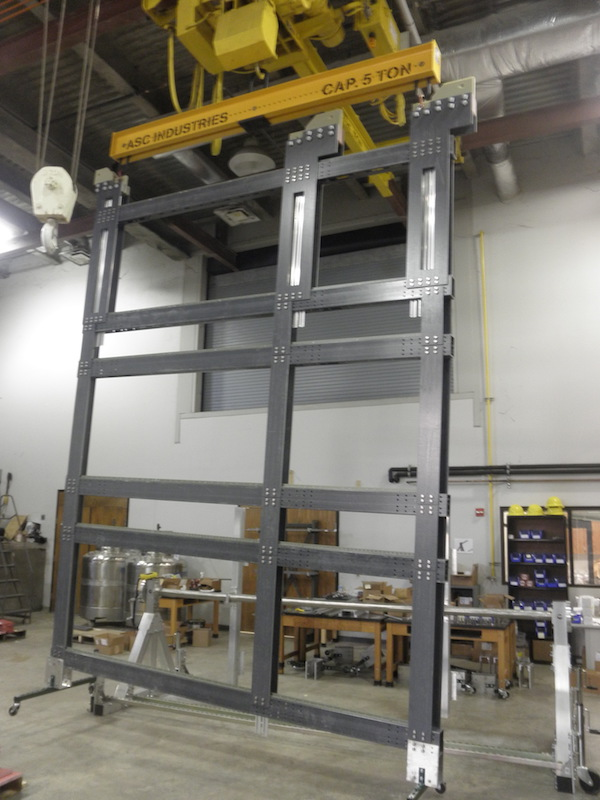
\includegraphics[width=0.7\textwidth]{3_fc_endwall_frames_hanging}
\end{dunefigure}


Aluminum profiles are inserted into the cutouts of the box beams and attached with screws and stainless steel slip nuts to L-shaped \dword{frp} brackets that are mounted on the \dword{frp} box beams. Small changes in part sizes will help to simplify the assembly  procedure with respect to the one used for \dword{pdsp}. Currently, we expect that pre-assembly of the \dword{fc} endwall frames will no longer be required. The full modules will be assembled at the factory (LSU), and then complete \dword{ewfc} panels will be shipped to the \dword{sdwf}. 



%%%%%%%%%%%%%%%%%%%%%%%%%%%%
\subsection{Electrical Interconnections}
\label{sec:fdsp-hv-prod-interconnect}

All electrical fasteners and wires used on the \dword{cpa} arrays and \dword{fc} are produced
to specification by commercial vendors and packaged with the \dword{cpa} or \dword{fc} modules.  
As discussed in Sections~\ref{sec:fdsp-hv-prod-cpa} and~\ref{sec:fdsp-hv-prod-fc}), 
this includes. e.g., the \dword{hv} cable segments, wire jumpers, and machined brass
tabs.

University shops will produce and test circuit boards for %DUNE 
\dword{hv} interconnections according to the same design used for \dword{pdsp}.  The \dword{fc} voltage dividers were produced for \dword{pdsp} at LSU, and the boards for \dword{cpa} frame bias and \dword{cpa}-\dword{fc} connections were produced at Kansas State University (KSU).
%\todo{What about the \dword{fc}-to-\dword{apa} boards?} 
Both institutions have created custom test apparatuses for verifying proper operation of the boards at full voltage and over-voltage conditions, keeping the boards free of solder flux and flux-remover.  These institutions may scale up production and testing by the required order of magnitude for the \dword{spmod} or share this work with other institutions, whichever best meets the needs of the project. %Each board is free of solder flux and flux-remover. (moved sentence up)

%%%%%%%%%%%%%%%%%%%%%%%%%%%%
\subsection{Production Safety}
\label{sec:fdsp-hv-prod-safety}

Production of the \dword{fc} panels and resistor-divider boards will involve collaboration technical, scientific, and student labor and  does not present unusual industrial hazards. The \dword{hvs} consortium will work closely with each production site to ensure that procedures meet both \dword{fnal} and institutional requirements for safe procedures, \dword{ppe}, environmental protection, trained materials handling, and training. The vast majority of production part fabrication will be carried out commercially and shipping will be contracted through approved commercial shipping companies. Prior to approving a site as a production venue, it will be visited and reviewed by an external safety panel to ensure best practices are in place and maintained. 

%Testing of the \dword{hv} feedthrough will be done in a closed cryostat to avoid exposure to high voltage.  Special attention will be given to the grounding between the power supply and cryostat. Tests are performed in a closed \dword{lar} cryostat to assure the nominal voltage is functional.  There is no exposed \dword{hv} during testing.  
Testing of the \dword{hv} feedthrough will be done in a closed cryostat to avoid exposure to high voltage and  to assure the nominal voltage is functional.  The power supply is grounded to the cryostat as a further safety measure. Tests for the \dword{pdsp} \dword{hv} feedthrough were done at \dword{cern} after a safety electrical and cryogenic review mainly focusing on the grounding of the whole test stand (power supply, cable, and cryostat where the feedthrough was tested) as well as interlocks. A safety document (PPSPS) was created, reviewed, and approved for this test. Similar testing and documentation will be done for the \dword{spmod}.


%%%%%%%%%%%%%%%%%%%%%%%%%%%%%%%%%%%%%%%%%%%%%%%%%%%%%%%%%%%%%%%%%%%%
\section{Quality Control, Transport, and Installation}
\label{sec:fdsp-hv-transport}

The \dword{hvs} consortium has developed a comprehensive quality control (\dword{qc})
plan for the production, shipping, and installation of the \dword{spmod} \dword{hv} components. %has been developed 
It is based partly on \dword{qc} procedures developed and implemented on \dword{pdsp} and on the \dword{nova} experiment's successful use of barcode tagging for identifying and tracking detector components.  Inventory tagging and tracking each component is crucial. Documentation in the form of printed checklists is maintained~\cite{bib:docdb10452}. 

Travelers have been replaced by a system of tags with bar codes attached to the units, which key to electronic \dword{qc} data. The tags will be large and brightly colored enough to be seen from both ends of the cryostat.
A particularly suitable choice is to use 
bright yellow cattle tags, plastic tags of about 10-12 square inches ($\sim\,\SI{70}{cm^{2}}$) on which a unique QR\footnote{Quick Response Code, The QR\texttrademark{} code system was invented in 1994 by the Japanese company Denso Wave. \url{https://www.qrcode.com/en/index.html}.} or bar code can be printed; they can be purchased very inexpensively in quantities of hundreds or thousands.


Scanned tags are removed after completion of electronic checklist forms linked to the tag's bar code.  At the end of \dword{tpc} installation, all \dword{qc} data for components at a particular location in the detector are stored electronically and linked to that location.



%%%%%%%%%%%%%%%%%%%%%%%%%%%%
\subsection{Quality Control}
\label{sec:fdsp-hv-transport-QC}

Power supply devices used in an \dword{spmod} will be tested before installation.  Output voltages and currents will be checked on a known load. 

The feedthrough and filters will be tested at the same time, with the selected power supply.  The feedthrough must be verified to hold the required voltage in \dword{tpc}-quality \dword{lar} ($\tau\geq$\SI{1.6}{ms}) for several days.  The ground tube submersion and \efield{} environment of the test setup will be comparable to the real \dword{fc} setup or more challenging (e.g., the test liquid level can be lower than that in the \dword{spmod} but not higher).  Additionally, the feedthrough must be leak-tight to satisfy cryogenics requirements.

The \dword{qc} tests concerning the voltage divider boards are as follows: All individual resistors and
 varistors are submitted to a warm and cold (87 K) current-voltage measurement. This forms the basis for selecting components that meet specifications: all
 electrical components must pass visual inspection for mechanical damage; all measurement values (resistance, clamping voltage) must be within 2$\,\sigma$ of the mean for entire sample both in warm and cold tests.

The \dword{qc} process for mechanical components starts at the production factories by attaching a cattle tag with a unique code to each production element.  A file linked to each code contains the individual measurements and properties contained in the \dword{qc} checklists for that element.  The following is an example of how this system will be implemented for the \dword{cpa} components:

\begin{enumerate}
\item During assembly, \dword{qc} checklists are filled out electronically using a smart phone or tablet.  Once a \dword{cpa} unit 
is completely assembled and all checklists are complete, a coded temporary cattle tag is attached and scanned, linking the checklist information to the code on the tag. (The \dword{cpa} unit's individual parts are not tagged separately.)
\item 
A shipping crate will contain six %2-module 
\dword{cpa} units, each with its removable coded tag, plus any included hardware packages, each with a coded sticker.
\item A coded label on the shipping crate (paper sticker) will %contain 
identify the contents of the crate (six codes + codes of hardware packages). The code on the label is used only for shipping purposes and for inventory purposes.  %at the \dword{itf}.
\item In the \dword{surf} cleanroom, the first \dword{cpa} panel is assembled. A coded tag is attached to the \dword{cpa} panel and scanned.  Then the three individual \dword{cpa} unit tags are scanned and removed, linking them to the \dword{cpa} panel code.
\item The same procedure is followed for the second \dword{cpa} panel from the crate.  Each \dword{cpa} panel now has a single tag attached to it.
\item The %next step is to combine 
\dword{cpa} panels are then combined into a \dword{cpa} plane, and a single coded tag is attached to the \dword{cpa} plane and scanned. % is attached to the Plane and scanned.  
The two individual \dword{cpa} panel tags are then scanned, linking their codes to the that of the \dword{cpa} plane. %Plane.
\item Top and bottom \dword{fc} modules 
are attached to both sides of the \dword{cpa} plane, and  a single coded tag is placed on this \dword{cpafc} assembly identifying the codes of each of the four \dword{fc} modules %(4 tags) 
and the code of the \dword{cpa} planes;  %CPA Plane (one tag) - 
these five tags are removed after scanning.  
\item When moving the panel into the cryostat the code of the position tag on the \dword{dss} is scanned as well as the tag on the \dword{cpafc} assembly, and then both tags %\dword{cpafc} 
are removed.
\end{enumerate}
At this point, %what is obtained is 
a sequence of linked codes associated with \dword{qc} checklists %that tell 
identify which \dword{cpa} and \dword{fc} modules %units 
are mounted in %the 
which \dword{dss} positions, and no tagging material remains in the cryostat.  A similar sequence is anticipated for the production of the top and bottom \dword{fc} units up to step 6; the endwalls are done separately but similarly.  
At the completion of installation in the cryostat and before top and bottom \dword{fc} deployment, visual inspection will confirm the absence of any tags.

%%%%%%%%%%%%%%%%%%%%%%%%%%%%
\subsection{Transport and Handling}
\label{sec:fdsp-hv-transport-transport}

The \dword{hvs} consortium has studied %issues of 
options for %the means of 
transportation from \dword{hvs} production sites %factories 
to the \dword{sdwf} %along with the type of 
and packaging of the shipped elements. 
We found that using reusable underground 
crates and returning them to the factories when empty is less expensive than using inexpensive, disposable crates for shipment from the factories to the \dword{sdwf},  
%It was found that the latter method was cheaper 
even with the extra shipment costs. %s of empty crates back to factories. 

We have identified a vendor that %was found which 
produces honeycombed PVC sheets of varying thicknesses that can be formed into crates. These %that 
can be loaded at the production sites, %factories, 
shipped to the \dword{sdwf}, and sent underground at \dword{surf}.  
We will require 50 shipments of crates containing two \dword{cpa} panels each to complete the \dword{spmod}.  %With the reusable underground crate scheme in place, only 20 crates are required to make the 50 shipments. 
The reusable underground crate scheme requires only 20 crates to make the 50 shipments. Similar reductions are obtained for the top and bottom \dword{fc} modules. 


Crates would be available at each factory at the start of production. 
As production proceeds, individual assembly units are bagged and sealed inside them.
When a full shipment of crates is ready at a factory, crates are sent by flatbed truck from the factory to the \dword{sdwf}.  The full crates are stored at the \dword{sdwf} until they can be received at SURF.  Some components may require \dword{qc} and/or minor assembly procedures to be done at the \dword{sdwf} before shipping to \dword{surf}.

At \dword{surf}, the crates are lowered into the staging area outside the cleanroom where they are unpacked. The assembly units are removed from their bags and taken into the cleanroom for installation. Only cleaned assembly units are allowed into the cleanroom; the crate is restricted to the staging area only. The empty crate is returned to the \dword{sdwf} and then sent back to a production factory for reloading. 



%%%%%%%%%%%%%%%%%%%%%%%%%%%%
\subsection{Safety during Handling} % Safety}
\label{sec:fdsp-hv-transport-safety}
%\subsection{Assembly and Installation}
%\label{sec:fdsp-hv-install}


In the current installation scenario, no assembly activities are foreseen at the \dword{sdwf} site for any components of the \dword{hv} system. Only visual inspection of the \dword{hvs} modules crate condition will be performed to verify the integrity after shipping. 
No disruption in installation should occur in the event of shipping damage since there is a one-month storage period at the \dword{sdwf} and two week's installation storage underground at \dword{surf}.  The \dword{hvs} consortium will coordinate procedures for underground handling with \dword{tc}.

A detailed Gantt chart on the production and installation schedule for the \dword{hvs} of the first \dword{spmod} is shown in Figure~\ref{fig:tasks}.

The installation activities are described in Chapter~\ref{ch:sp-install}.

%%%%%%%%%%%%%%%%%%%%%%%%%%%%%%%%%%%%%%%%%%%%%%%%%%%%%%%%%%%%%%%%%%%%
\section{Organization and Management}
\label{sec:fdsp-hv-org}

%%%%%%%%%%%%%%%%%%%%%%%%%%%%

\subsection{Institutional Responsibilities}
\label{sec:fdsp-hv-org-consortium}
The \dword{hvs} consortium %has consolidated 
includes all the institutions that have participated in the design, construction, and assembly of the \dword{hv} systems for both \dword{pdsp}  and \dword{pddp}. They are listed in 
Table~\ref{tab:instit}. 
The consortium  currently comprises several USA institutions and \dword{cern}, %presently 
the only non-USA participant. 
 
  
As it has been %in the case of 
for \dword{protodune}, \dword{cern} is heavily committed to a significant role in the  \dword{fd} in terms of funding, personnel, 
 and the provision of infrastructure for R\&D and detector optimization. Moreover, \dword{cern} will be responsible for a significant fraction of subsystem deliverables; as such  \dword{cern} is actively in search of additional European institutions to attract into the consortium. 
 
At present, in the \dword{hv} current consortium organization, each institution is naturally assuming the same responsibilities that it assumed for %the developments of 
\dword{pdsp} and \dword{pddp}. The %present 
consortium organizational structure includes a scientific lead (from \dword{cern}), a technical lead (from BNL), %a \dword{tdr} editor (from \dword{fnal}), 
and an \dword{hvs} design and integration lead (from \dword{anl}). 

The successful experience gained with the \dword{pdsp} detector has demonstrated that the present \dword{hvs} consortium organization and the number of institutions are appropriate for the construction of the \dword{hv} system of the \dword{spmod}. Funding and the predominant participation of USA institutions are presently open issues that would benefit from more international participation. %The extension to non-USA institutions would be beneficial for both of these issues. 

 The consortium is organized into working groups (``WG'' below) addressing the design and  R\&D phases of development, and the hardware production and installation.

\begin{itemize}
\item WG1: Design optimization for \dword{spmod} and \dword{dpmod}; assembly, system integration, detector simulation, physics requirements for monitoring and calibrations; %Conveners: Jeff Nelson, Vic Guarino, Bo Yu
\item WG2: R\&D activities, R\&D facilities; %Conveners: Francesco Pietropaolo, Ting Miao
\item WG3: \dword{sp}-\dword{cpa}: Procurement of resistive panels, frame strips, electrical connections of planes; assembly, \dword{qc} at all stages, and shipment of these parts; \item WG4: \dword{dp} cathode and \dword{gp}:  material procurement; construction, assembly, shipment to \dword{sdwf} %ITF 
\dword{qa}, \dword{qc}; % Convener: Jae Yu
\item WG5:  modules: \dword{sp}-top/bottom-\dword{fc} module, \dword{sp}-endwall modules, \dword{dp}-\dword{fc} modules: procurement of mechanical and electrical components, assembly and shipping to \dword{sdwf}; and  %ITF. %Conveners: Thomas Kutter, Michael Wilking, Jeff Nelson, Jae Yu
\item WG6: \dword{hv} supply and filtering, \dword{hv} power supply and cable procurement, R\&D tests, filtering and receptacle design and tests. %Conveners: Franco Sergiampietri, Sarah Lockwitz
\end{itemize}

Taking advantage of identified synergies, some activities of the \dword{sp} and \dword{dp} working groups are merged: \dword{hv} feedthrough, voltage dividers, aluminum profiles, \dword{frp} beams, and assembly infrastructure.



\begin{dunetable}
[HVS consortium institutions]
%{p{0.50\textwidth}p{0.15\textwidth}}
{ll}
{tab:instit}
{Institutions participating in the \dword{hvs} consortium}   
Institution & Country \\ \toprowrule%(Contact, E-mail) 

\dword{cern} & Switzerland \\ \colhline%(Francesco Pietropaolo; francesco.pietropaolo@cern.ch) 
Argonne National Lab& USA \\ \colhline%(Steve Magill; srm@anl.gov) 
Brookhaven National Lab& USA \\ \colhline%(Bo Yu; yubo@bnl.gov) 
University of California Berkeley / LBNL & USA \\ \colhline%(Cheng Ju Lin; cjslin@lbl.gov)
 University of California Davis& USA \\ \colhline%(Emilja Pantic; pantic@ucdevis.edu) 
\dword{fnal} & USA \\ \colhline%(Sarah Lockwitz; lockwitz@fnal.gov) 
University of Houston & USA \\ \colhline%(Andrew Renshaw; arenshaw@central.uh.edu) 
Kansas State University& USA \\ \colhline%(Glenn Horton-Smith; gahs@ksu.edu)
Louisiana State University & USA \\ \colhline%(Thomas Kutter; kutter@phys.lsu.edu) 
%10 & South Dakota School of Mines and technology, USA (Juergen Reichenbacher; Juergen.Reichenbacher@sdsmt.edu) 
 SUNY Stony Brook & USA \\ \colhline%(Michael Wilking; michael.wilking@stonybrook.edu) 
 University of Texas Arlington & USA \\ \colhline%(Jaehoon Yu; jaehoonuy1@gmail.com) 
 Virginia Tech& USA \\ \colhline %(Jon Link; jmlink@vt.edu) 
College of William and Mary& USA \\ %(Jeff Nelson; jknels@wm.edu)  
\end{dunetable}
%%%%%%%%%%%%%%%%%%%%%%%%%%%%
\subsection{Risks}
\label{sec:fdsp-hv-org-risk}

Table~\ref{tab:risks:SP-FD-HV} presents a summary of the risk items identified for the \dword{hv} system of  the \dword{fd} \dword{spmod}. 


% risk table values for subsystem SP-FD-HV
\begin{footnotesize}
%\begin{longtable}{p{0.18\textwidth}p{0.20\textwidth}p{0.32\textwidth}p{0.02\textwidth}p{0.02\textwidth}p{0.02\textwidth}}
\begin{longtable}{x{0.18\textwidth}x{0.20\textwidth}x{0.32\textwidth}x{0.02\textwidth}x{0.02\textwidth}x{0.02\textwidth}} 
\caption[Risks for SP-FD-HV]{Risks for SP-FD-HV (P=probability, C=cost, S=schedule) More information at \dword{riskprob}. \fixmehl{ref \texttt{tab:risks:SP-FD-HV}}} \\
\rowcolor{dunesky}
ID & Risk & Mitigation & P & C & S  \\  \colhline
RT-SP-HV-01 & Open circuit on the field cage divider chain & Component selection and cold tests. Varistor protection. & L & L & L \\  \colhline
RT-SP-HV-02 & Damage to the resistive Kapton film on CPA & Careful visual inspection of panel surfaces.  Replace panel if scratches are deep and long  & L & L & L \\  \colhline
RT-SP-HV-03 & Sole source for Kapton resistive surface; and may go out of production & Another potential source of resistive Kapton identified. Possible early purchase if single source. & M & L & L \\  \colhline
RT-SP-HV-04 & Detector components are damaged during shipment to the far site  & Spare parts at  LW. FC/CPA modules can be swapped and replaced from factories in a few days. & L & L & L \\  \colhline
RT-SP-HV-05 & Damages (scratches, bending) to aluminum profiles of Field Cage modules & Require sufficent spare profiles for substitution. Alternate: local coating with epoxy resin. & L & L & L \\  \colhline
RT-SP-HV-06 & Electric field uniformity is not adequate for muon momentum reconstruction  & Redundant components; rigorous screening. Structure based on CFD. Calibration can map E-field. & L & L & L \\  \colhline
RT-SP-HV-07 & Electric field is below goal during stable operations & Improve the protoDUNE SP HVS design to reduce surface E-field and eliminate exterior insulators. & M & L & L \\  \colhline
RT-SP-HV-08 & Damage to CE in event of discharge  & HVS was designed to reduce discharge to a safe level. Higher resistivity cathode could optimize. & L & L & L \\  \colhline
RT-SP-HV-09 & Free hanging frames can swing in the fluid flow  & Designed for flow using fluid model; Deformation can be calibrated by lasers or cosmic rays. & L & L & L \\  \colhline
RT-SP-HV-10 & FRP/ Polyethene/ laminated Kapton component lifetime is less than expected & Positive experience in other detectors. Gain experience with LAr TPC's; exchangeable feedthrough. & L & L & L \\  \colhline
RT-SP-HV-11 & International funding level for SP HVS too low & Cost reduction through design optimization. Effort to increase international collaboration. & M & M & M \\  \colhline
RT-SP-HV-12 & Underground installation is more labor intensive or slower than expected & SWF contingency, full-scale trial before installation. Estimates based on ProtoDUNE experience. & L & L & L \\  \colhline

\label{tab:risks:SP-FD-HV}
\end{longtable}
\end{footnotesize}

The first five risks refer to the construction and operation phases; risks 6 through 12  apply to the installation  and/or  detector operation phase. 

Most of the cited risks have already been addressed during the construction, commissioning, and operation of \dword{pdsp}. 
None have caused significant problems, with the partial exception of risk 9. %item [ID09]. 
%Item [ID08] 
Risk 9 requires an accurate analysis of collected muon data (this activity is in progress), and the disentangling of space charge effects. 


Given the much larger detector scale and the more complex underground installation environment, the listed risks still %persist for 
apply to the \dwords{detmodule}. However, the positive experience gained with \dword{protodune} justifies the low risk probabilities assigned to most of the items.  To better justify these statements, brief explanations are given below, together with the identified mitigation actions.

Risk 1: An open circuit on the \dword{fc} could occur if a resistor in the conventional voltage dividers were to fail in the open condition, which %. Such a scenario 
could result in \dword{hv} discharges across the open circuit gap. Mitigation: Perform stringent component selection and cryogenic testing. Use parallel resistor chains to provide redundancy. Varistors, capable of withstanding several thousand amperes of current impulses, have been added in parallel with the resistor chains to protect them from large current surges. Check resistances %will be checked 
several times during \dword{fc} fabrication and assembly phases, including once after the \dword{fc} deployment.   

Risk 2: Limited, local scratches could %possibly 
occur from accidental contacts during module assembly or installation. No mitigation is required if a scratch is limited in size. For larger scratches that can induce delamination, the mitigation is to replace the panel with a spare. 

Risk 3: About 12 rolls of resistive Kapton are needed (\SI{4}{ft} wide, \SI{300}{m} per roll)  for the \dword{cpa} panels of one \dword{spmod}.  The cost is 20k\$ per roll from the only vendor available up to now. Mitigation: Recently another source of resistive Kapton has become available and is being investigated. An early purchase is also under consideration in case of a single source condition.

Risk 4: Poor shipping techniques could cause damage to delicate components (e.g., broken \dword{cpa} panels, bent or heavily scratched aluminum profiles) that would cause the modules to fail \dword{qc} tests. 
If significant repairs to detector components are needed, they may require replacements.   Mitigation: Plan for an adequate number of spare elements and implement 
a documented \dword{qa} program for shipment packing with detailed review of shipping procedures, shipping containers, and testing in crates after arrival.

Risk 5: The surface of the aluminum profiles is very delicate and deep scratches could locally increase the \efield to close to the critical field of \SI{30}{\kV}/cm. The surface can be damaged during transport or manipulation in the assembly area. In case of significant damage, it cannot be repaired due to its conductive coating. For mitigation, ensure the availability of sufficient spare profiles %are required  
on-site to allow last-minute substitutions. Alternatively, use a local coating with epoxy resin. % could be used.

Risk 6: Unexpected changes in \dword{fc} resistor values, cathode/\dword{fc} non-planarity or movement, and surface or space charge buildup can distort the \efield. As a consequence, the momentum of non-contained muons,  measured by estimating the multiple scattering rate for the observed track segments, could be incorrectly estimated, thereby degrading %. This would degrade 
the momentum resolution for non-contained muons.  ${\nu}_{\mu}$ disappearance analyses and three-flavor fits could be affected %and there can be 
leading to feed-down of high-energy neutrino backgrounds to low-energy reconstructed categories.  Mitigation: Consider addition of a laser calibration %will be considered 
if calibration with cosmic crossing muons is not sufficient. 

Risk 7:  In \dword{protodune}, \dword{hv} instabilities appeared as current streams occurring at intervals of several hours and localized on  a specific \dword{fc} module. These required a several-minute ramp-down of the \dword{hv} from the nominal \SI{-180}{kV} to a lower value, typically \SI{-140}{kV}; see Section~\ref{sec:fdsp-hv-protodune}.
Investigations are underway to characterize and mitigate this risk. Recently, understanding of this risk has significantly progressed thanks to the 
long-term operation of \dword{pdsp} in 2019 while exposed only to cosmic rays. 
There are strong hints %confirming  (Anne: strong hints do not confirm ;-)  )
that the instabilities are due to charging-up processes on insulators. In addition, %there is confirmation that 
the current streamers are confirmed to have been localized mainly on %a single 
one \dword{gp} (of 12). No degradation of the detector performance due to \dword{hv} instabilities has been observed. %On the contrary, 
Moreover, these instabilities appear to decrease gradually in rate and intensity. At present, the detector down-time due to these instabilities is less than 1\%.  

\dword{protodune} long-term operation is also indicating that \dword{lar} purity does not  play a significant role in the onset of the \dword{hv} instability (for free electron lifetime above $\sim\,$\SI{1}{ms}).  The impact of the \dword{hv} instabilities on \dword{apa}/\dword{ce} and \dwords{pd} is also under investigation and at the moment appears to be negligible.

The mitigation for risk 7 involves improvement at the design level to increase as much as possible the distance between the \dword{fc} and \dwords{gp} and to avoid high-field regions by smoothing all electrodes exposed to \dword{hv}.  %ProtoDUNE NP02, 
\dword{pddp}, with a comparable design, will help determine %understanding 
the validity of these improvements.

Risk 8: A sudden discharge on the \dword{hv} system would inject charge to the \dword{fe} \dwords{asic}, overwhelming the protection circuits and causing permanent damage. Mitigation: Key aspects of the \dword{hvs} design were aimed at reducing the charge injection to a safe level for the \dword{ce}, such as segmenting the \dword{fc} and making the cathode planes resistive.  We are still searching for higher-resistivity material on the cathode to increase the safety factor. 

Risk 9:  Each cathode is made of lightweight, non-porous material with an area of \SI{58x12}{m} that could move under the  convectional flow of the \dword{lar}.  Mitigation: The \dword{cpa} structure is designed to withstand pressure from \dword{lar} flow based on fluid model predictions. Static deformation can be calibrated by lasers or cosmic rays.

Risk 10: Aging of insulator components in \dword{lar} could %be an issue
pose a problem,  but  experience in \dword{atlas} (Kapton \& PCB, $20+$ years), \dword{icarus} (G10, feedthrough $4+$ years; feedthrough exchangeable) is trending favorably. Mitigation: %More experience will be gained . 
Continue to gain experience with \dwords{lartpc}. Make feedthrough exchangeable.

Risk 11: Current costing suggests that international funding could be %a potential issue.
insufficient. Mitigation: Implement cost reduction through design optimization and scaling. Make efforts to include more international %collaboration 
institutions. 

Risk 12: Underground installation is more labor-intensive or slower than expected. Mitigation: Add labor contingency. Carry out full-scale installation trials at the  \dword{ashriver} site prior to installation. The estimates are based on \dword{protodune} experience. With the present knowledge, the \dword{hv} system is not on the critical path for installation.

%%%%%%%%%%%%%%%%%%%%%%%%%%%%
\subsection{High-level Schedule}
\label{sec:fdsp-hv-org-cs}

Table~\ref{tab:HVsched} lists the most high-level milestones for the design, testing, production, and installation of the \dword{spmod} \dword{hvs}. Dates in this tentative schedule are based on the assumed start of installation of the first \dword{spmod} at \dword{surf}. The dates for the \dword{hvs} production of a second \dword{spmod} are %also 
included as a reference.

 The production scenario %assumed 
 for the schedule presented in Table~\ref{tab:HVsched} assumes %is based on 
 two factory sites for the \dword{cpa} construction, two for the top/bottom \dword{fc} modules and one for \dword{ewfc} modules. Given the present starting date % for installation underground of
 for  the first \dword{spmod} installation, this assumption is fully compatible with the time available after the operation of the \dword{protodune2} prototype.
 A more detailed schedule for production and installation of the first \dword{spmod} is found in %the Gantt chart provided in 
 Figure~\ref{fig:tasks}.

\begin{dunetable}
[HVS consortium schedule]
{p{0.65\textwidth}p{0.25\textwidth}}
{tab:HVsched}
{High level Milestones and Schedule for the production of the \dword{hvs} of the \dword{spmod}}   
Milestone & Date (Month YYYY)   \\ \toprowrule
Technology Decision &      \\ \colhline
CPA/FC/Endwall 60\% Design Review & June 2019 \\ \colhline
CPA/FC/Endwall Mod 0 (for tests at \dshort{ashriver}) & June 2019 - June 2020 \\ \colhline
Final Design Review & June 2020     \\ \colhline
Start of module 0 component production for  \dshort{protodune2} & June 2020     \\ \colhline
End of module 0 component production for  \dshort{protodune2} &  March 2021    \\ \colhline
\rowcolor{dunepeach} Start of  \dshort{protodune2} installation& \startpduneiispinstall      \\ \colhline
\rowcolor{dunepeach} Start of  \dshort{protodune2} installation& \startpduneiidpinstall      \\ \colhline
\rowcolor{dunepeach}South Dakota Logistics Warehouse available& \sdlwavailable      \\ \colhline
\rowcolor{dunepeach}Beneficial occupancy of cavern 1 and \dshort{cuc}& \cucbenocc      \\ \colhline
\rowcolor{dunepeach}  \dshort{cuc} counting room accessible& \accesscuccountrm      \\ \colhline
 Top/Bottom FC  \dshort{prr} & July 2023    \\  \colhline
 Start of Top/Bottom FC production  & September 2023     \\ \colhline
CPA  \dshort{prr} &  October 2023    \\ \colhline
Start of  \dshort{cpa} production  & December 2023     \\ \colhline
\rowcolor{dunepeach}Top of  \dshort{detmodule} \#1 cryostat accessible& \accesstopfirstcryo      \\ \colhline
 Endwall FC  \dshort{prr} & February 2024     \\  \colhline
Start of Endwall FC production  & April 2024     \\ \colhline
End of  \dshort{cpa} production Detector \#1 & August 2024     \\ \colhline
End of Top/Bottom FC production Detector \#1 & August 2024  \\ \colhline
End of Endwall FC production  Detector \#1 & August 2024  \\ \colhline
\rowcolor{dunepeach}Start of  \dshort{detmodule} \#1 TPC installation& \startfirsttpcinstall      \\ \colhline
\rowcolor{dunepeach}Start of  \dshort{detmodule} \#1 TPC installation& \startfirsttpcinstall      \\ \colhline
\rowcolor{dunepeach}Top of  \dshort{detmodule} \#2 accessible& \accesstopsecondcryo      \\ \colhline
\rowcolor{dunepeach}End of  \dshort{detmodule} \#1 TPC installation& \firsttpcinstallend      \\ \colhline
 \rowcolor{dunepeach}Start of  \dshort{detmodule} \#2 TPC installation& \startsecondtpcinstall      \\ \colhline
End of  \dshort{cpa} production Detector \#2 & September 2025  \\ \colhline
End of Top/Bottom FC production Detector \#2  &  October 2025   \\ \colhline
End of Endwall FC production Detector \#2  & January 2026  \\  \colhline
\rowcolor{dunepeach}End of  \dshort{detmodule} \#2 TPC installation& \secondtpcinstallend      \\ 
\end{dunetable}


\begin{dunefigure}[HVS production and installation schedule for first SP detector module]{fig:tasks}{
Gantt chart providing a detailed view of the production and installation schedule for the \dword{hvs} for the first \dword{spmod}.}
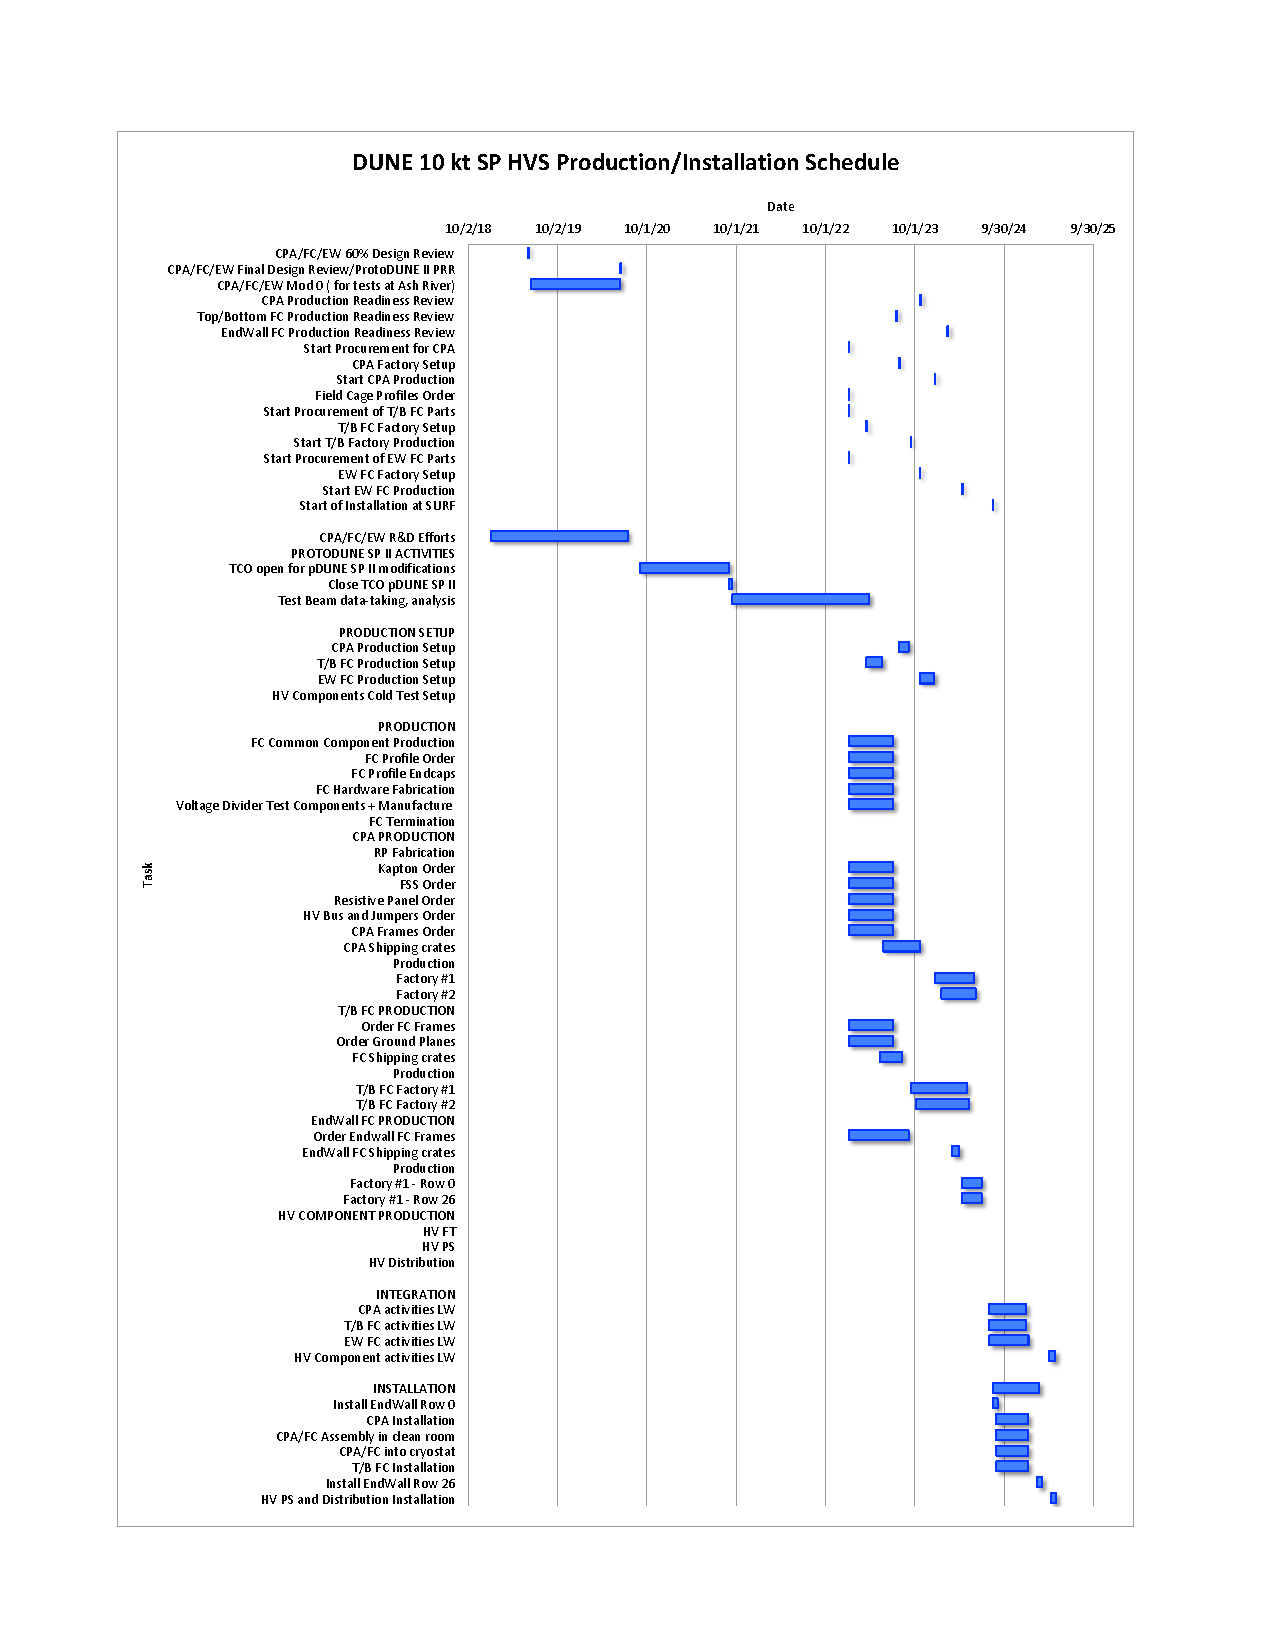
\includegraphics[width=0.95\textwidth]{graphics/HVS-GANTT-new.pdf}
\end{dunefigure}





%%%%%%%%%%%%%%%%%%%%%%%%%%%%%%%%%%%%%%%%%%%%%%%%%%%%%%%%%%%%%%%%%%%%

\section{Appendix: Alternatives}
\label{sec:fdsp-hv-app-alt}

\subsection{Optical Reflectors on CPA}
\label{sec:fdsp-hv-app-alt-opt}

Since the \dwords{pd} in the current \dword{tpc} design are installed only on the \dword{apa} side of the drift volume and have low coverage, their responses to ionization inside the \dword{tpc} are highly dependent on drift distance and severely biased toward the \dword{apa}.  In order to improve the uniformity of response along the drift direction, the \dword{pd} consortium has proposed adding reflector foils coated with \dword{wls} to convert the UV photons arriving at the cathode into visible photons and bounce them back to the \dwords{pd} inside the \dword{apa}s.  Simulations have shown that addition of the reflectors  significantly improves the uniformity of response.

Implementing this concept, however, could dramatically alter the current \dword{cpa} characteristics and design.  The \dword{hvs} consortium has %Several concepts have been developed by the HVS 
developed several concepts to accommodate the reflectors with minimal change to the %current 
\dword{cpa} design.  The main issue %here 
is the conductivity of the reflector foil versus the highly resistive nature of the \dword{cpa}.  To improve the light output, it would be best to %One would like to 
cover as much of the cathode surfaces as possible, but % if the reflectors are conductive, aluminum-coated for example, large area coverage with these 
large area coverage with conductive, (e.g., aluminum-coated) reflectors could short-circuit the resistive cathode and render it ineffective in slowing down the energy transfer during a potential \dword{hv} breakdown.  On the other hand, %if the reflector foils are insulators, they would intercept the ionization drifting toward the cathode and become charged.  
reflector foils made of insulating material would intercept the ionization charges drifting toward the cathode and become charged. This would alter the drift field uniformity and, worst yet, could result in random breakdown through the foil.

A design concept that is fairly simple to implement %and that uses a known material 
is depicted in Figure~\ref{fig:reflectorOnCPA}.  A 3M Vikuiti\footnote{Vikuiti\texttrademark is a light enhancement film produced by the 3M Company,  \url{http://multimedia.3m.com/mws/media/419882O/vikuititm-rear-projection-displays-brochure.pdf}.} 
reflector foil or equivalent is laminated onto a thin \frfour backing sheet to maintain thermal expansion compatibility
with the resistive \dword{cpa} panel, which also has an \frfour core. The reflector foil assembly is perforated at regular intervals to allow %electrons to be collected 
collection of electrons through the holes to the \dword{rp}  surface, minimizing the voltage build-up from charging of the non-perforated surfaces.  Several such foil assemblies are then tiled onto the existing \dwords{rp} with screws.

In order to advance the \dword{cpa} design while providing the option of adding the reflector foils at a later time, the \dword{hvs} consortium will design %in 
a hole pattern 
on the %\dword{cpa} resistive panels
\dwords{rp} that could be used for mounting of reflector foils or panels, or left unused without negative consequences. In the meantime, \dword{hvs} and \dword{pd} consortia are conducting joint R\&D to evaluate a few design concepts and material choices. 


\begin{dunefigure}[Concept to attach reflector to a CPA panel]{fig:reflectorOnCPA}{A concept to attach reflector foils to a \dword{cpa} panel. (Credit: BNL)}
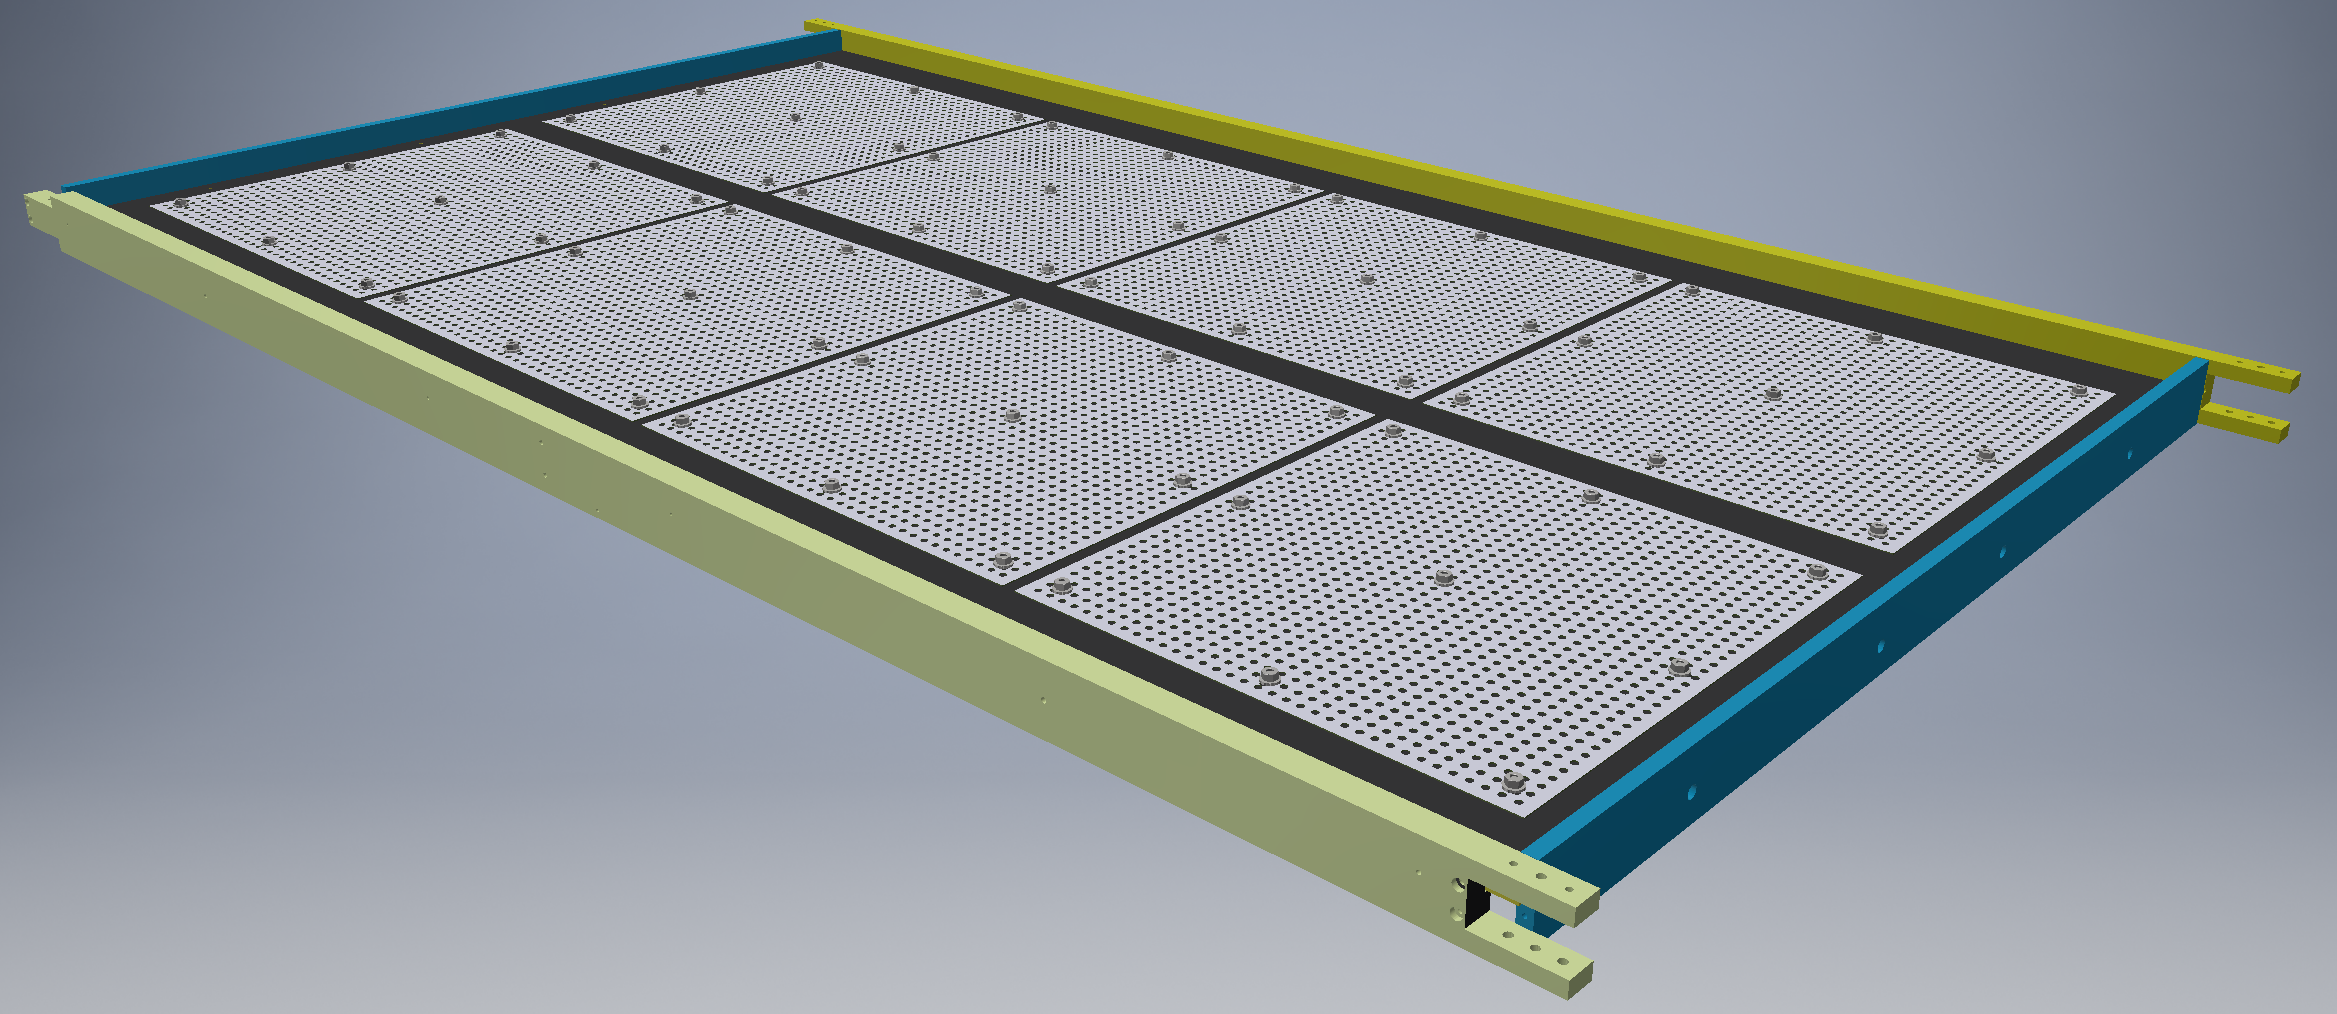
\includegraphics[width=0.9\textwidth]{ReflectorOnCPA.png}
\end{dunefigure}

\subsection{Calibration Laser Penetrations}
\label{sec:fdsp-hv-app-alt-cal}

The calibration consortium is developing requirements for calibrating the \efield.  One existing technique is to use UV laser beams to ionize the \dword{lar} and generate straight tracks along known trajectories.  Because the \dword{fc} surrounds the \dword{tpc} active volume, we can either shoot through the gaps between the \dword{fc} profiles (as in \dword{microboone}) or make openings in the \dword{fc} for the laser heads to pass through (as in \dword{sbnd}). Figure~\ref{fig:SBND_laser}  shows the design of a corner of the \dword{sbnd} \dword{tpc} with a \dword{fc}  opening and a calibration laser head through the opening.  Implementing such openings is straightforward if the openings are at the \dword{fc}  module boundaries.  Doing so through the interior surface of a \dword{fc} panel is more complicated but still simpler than the beam plug we designed for \dword{pdsp}.  There will be some minor drift field distortion around the openings.  Preliminary \dword{fea} studies have shown the field distortion to be negligible. 

\begin{dunefigure}[SBND laser arrangement]{fig:SBND_laser}{SBND field cage opening to allow a calibration laser head to pass through. (Credit: BNL)}
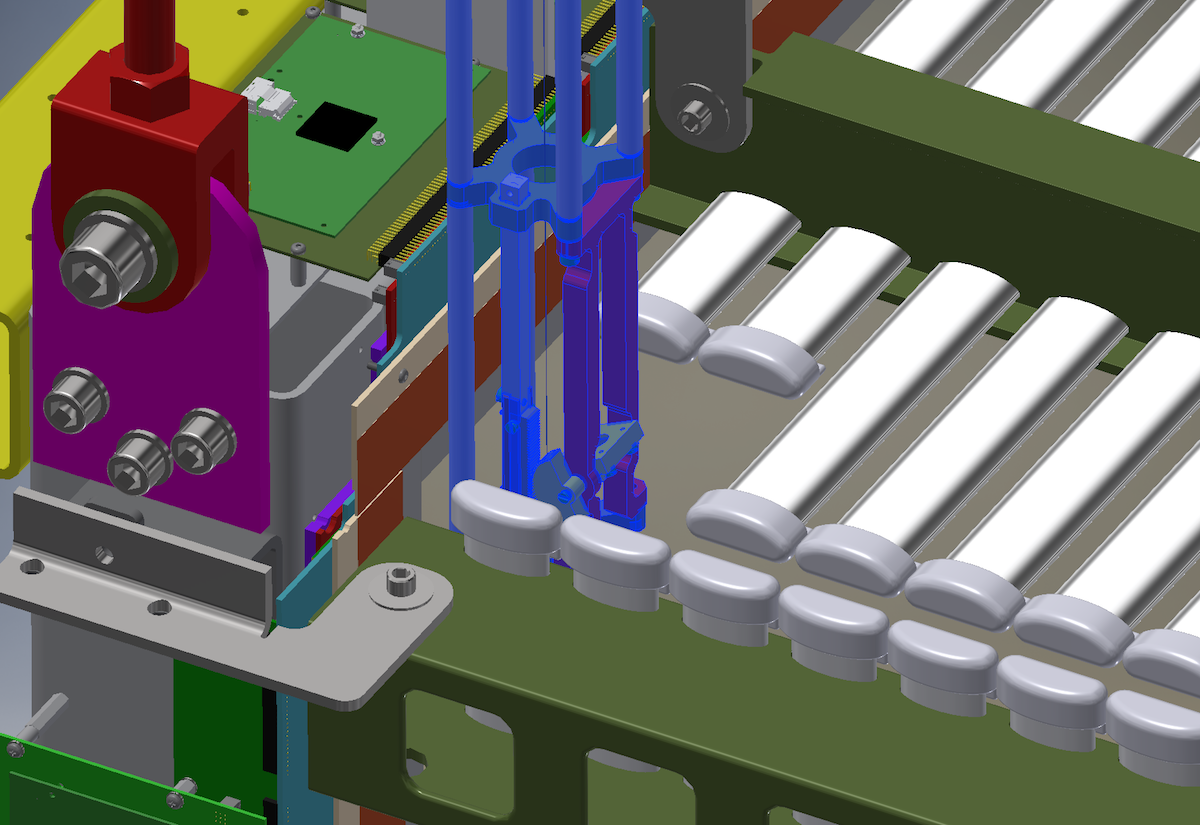
\includegraphics[width=0.7\textwidth]{SBND_Laser_Arrangement.png}
\end{dunefigure}


